% nur_msuthesis.tex
\documentclass{msuthesis}
%\usepackage[light,first]{draftcopy} %remove for final version

% book design declarations------------
\usepackage{times}
\usepackage{graphicx}
\usepackage{color}
\usepackage{subfigure}
\usepackage[hang,labelsep=quad,singlelinecheck=no]{caption}


%default SubSubSection is lowest section level \setcounter{tocdepth}{3}
\settowidth{\maxchapwidth}{\normalfont XVII.} 
\settowidth{\maxsectwidth}{\normalfont 0.0} 
\settowidth{\maxsubsectwidth}{\normalfont 0.0.0} 
\settowidth{\maxsubsubsectwidth}{\normalfont 0.0.0.0} 
\settowidth{\maxtabnowidth}{0.0}
\settowidth{\maxfignowidth}{0.0}

\usepackage{setspace}
%%% bibliography definitions %%%%
\newcommand{\biblist}{nur_thesis} 

%%% Front matter info %%%
%maximum 3 title lines on title page
\renewcommand{\booktitle}{Effective Kaon-Nucleon Cross Section from Nuclear Transparency Measured in the $A(e,e^\prime K^+)$ Reaction}
\renewcommand{\booktitletwo}{}
%\renewcommand{\booktitlethree}{in the Hall-C of Thomas Jefferson National Accelerator Facility}
%default abstracttitle is all booktitle lines on one line
\renewcommand{\authorname}{Nuruzzaman}
\renewcommand{\doctype}{Thesis Dissertation} %Dissertation, project, whatever you like
%default university is Mississippi State University
%default city is Mississippi State
%default state is Mississippi
%\setlength{\figwidth}{0.4\linewidth}
%\Figure{MSU_logo}{\figwidth}{}
\renewcommand{\department}{Department of Physics and Astronomy}
\renewcommand{\major}{Physics}
\renewcommand{\majorprofessor}{Dr. Dipangkar Dutta}
\renewcommand{\thesisdirector}{} %default thesisdirector is same as major professor
\renewcommand{\degree}{Master of Science}
\renewcommand{\degreemonth}{August}
\renewcommand{\degreeday}{7}
\renewcommand{\degreeyear}{2010}
\renewcommand{\kwlist}{%    %%%MSU 5/17/07%%% keywords allowed
thesis, 
dissertation, 
LaTeX, 
book design, 
format, 
template
}
%%% other definitions %%%%%
\renewcommand{\listofsymbolsname}{List of Symbols, Abbreviations, and Nomenclature}

\begin{document}  %%%%%%%%%%%%%%%%%%%%%%%%%%%%%%%%%%%%%%%%%%%%%%
\frontmatter %%%%%%%%%%%%%%%%%%%%%%%%%%%%%%%%%%%%%%%%%%%%%%%%%%%
\maketitlepage
\copyrightpage    %MSU recommended%%%p.15

%default \setlength{\sigwidth}{2.8in}
%default \setlength{\sigheight}{0.5in}
% this command adjusts the distance from the title to the author's
% name. if you have <= 6 signatures, you shouldn't need to change
% this. if you have more than 6, you can set this to something smaller
% to leave more space for signatures
\setlength{\sigtitletoauthor}{0.8in} % this is the default value
% this one sets the distance from the author name to the word
% ``approved'', for the same purpose as \sigtitletoauthor
\setlength{\sigauthortoapproved}{0.3in} % this is the default value

\approvals
\begin{center}
\noindent
\signature{%
Dipangkar Dutta
}{Assistant Professor of Department 
}{of Physics and Astronomy
}{(Major Professor)
}
\hfill
\signature{%
James A. Dunne
}{Professor of Department 
}{of Physics and Astronomy
}{(Committee Member)
}
\\
%\signature{%
%Anatoli Afanasjev
%}{Associate Professor of Department 
%}{of Physics and Astronomy
%}{(Committee Member)
%}
%\hfill
\end{center}


\begin{center}
\noindent
\signature{%
David L. Monts
}{Professor of Department 
}{of Physics and Astronomy
}{and Graduate Coordinator
\\(Committee Member)}
\hfill
\signature{%
Gary Myers
}{Dean of Arts and Sciences
}{}
{}
\end{center}
%%% MSU 4/23/08 Dean's name even though associate dean signs

\abstractpage

The Q-weak experiment in Hall-C at the Thomas Jefferson National Accelerator Facility has made the first direct measurement of the weak charge of the proton through the precision measurement of the parity-violating asymmetry in elastic electron-proton scattering at low momentum transfer. 
There is also a parity conserving Beam Normal Single Spin Asymmetry or transverse asymmetry ($B_{n}$) on $H_{2}$ with a sin($\phi$)-like dependence due to two-photon exchange. If the size of elastic $B_{n}$ is a few ppm, then a few percent residual transverse polarization in the beam, combined with small broken azimuthal symmetries in the detector, would require a few ppb correction to the Q-weak data. As part of a program of $B_{n}$ background studies, we made the first measurement of $B_{n}$ in the N-to-$\Delta$(1232) transition using the Q-weak apparatus. 
The final transverse asymmetry, corrected for backgrounds and beam polarization, was found to be $B_{n}$ = 42.82 $\pm$ 2.45 (stat) $\pm$ 16.07 (sys)~ppm at beam energy $E_{beam}$ = 1.155~GeV, scattering angle $\theta$ = 8.3\degrees{}, and missing mass $W$ = 1.2~GeV.
%This dissertation presents the analysis of the first measurement of the beam normal single spin asymmetry in inelastic electron-proton scattering at a $Q^{2}$ of 0.0209 (GeV/c)$^{2}$. 
$B_{n}$ from electron-nucleon scattering is a unique tool to study the $\gamma^{*}\Delta\Delta$ form factors, and this measurement will help to improve the theoretical models on beam normal single spin asymmetry and thereby our understanding of the doubly virtual Compton scattering process.


%The electron-proton scattering rate largely depends on the five beam parameters: horizontal position, horizontal angle, vertical position, vertical angle, and energy. Changes in these beam parameters when the beam polarization is reversed create false asymmetries. Although attempt has been made to keep changes in beam parameters during reversal as small as possible, it is necessary to correct for such false asymmetries. 

To help correct false asymmetries from beam noise, a beam modulation system was implemented to induce small position, angle, and energy changes at the target to characterize detector response to the beam jitter.
Two air-core dipoles separated by $\sim$10~m were pulsed at a time to produce position and angle changes at the target, for virtually any tune of the beamline. The beam energy was modulated using an SRF cavity. 
The hardware and associated control instrumentation will be described in this dissertation. 
Preliminary detector sensitivities were extracted which helped to reduce the width of the measured asymmetry. The beam modulation system has also proven valuable for tracking changes in the beamline optics, such as dispersion at the target.



% %%%MSU 5/17/07%%%% the following logic is for optional key words
%                    If kwlist is empty, then keywords line is not printed.
\settowidth{\tmplen}{\kwlist}
\ifthenelse{%
\lengthtest{\tmplen > 0pt}%
}{%
\par
\vspace{\baselineskip}        
%\noindent Key words: \kwlist
}{}%
%%%end MSU 5/17/07 %%%


%Correct page numbering requires 
%either \dedication or \acknowledgments\setcounter{page}{2}
%default is to make Dedication page ii

\dedication       %MSU%%%required here for correct page numbering. Guidelines says optional%%%p.16
\begin{center}
To my parents Md. Shamsuzzoha, Nurun Nahar and my sister Arjun Nahar and my dearest friend Shampa Samanta,\\

And

My teacher Probodh Mondal, Malay Dutta, Subroto Kundu and Dipangkar Dutta
\end{center}

\acknowledgments  %MSU optional%%%p.16 but not optional for this template
%Uncomment this \setcounter if there is no dedication
%\setcounter{page}{2} %MSU%%%title page is page 1, other pages not counted

% exack.tex Acknowledgments
%
This experiment was sponsored by the Department of Energy Office of Science Grant No.: DE-FG02-07ER41528. I am very grateful for the support I received and the opportunities that were available during this time. I am indebted to seemingly countless people for what I have accomplished and, first of all, I would like to say thank you to all of these people.

My supervisor, Dr. Dipangkar Dutta, provided me with many opportunities and I am deeply grateful for his support through the entire process. When I first joined the Mississippi State University graduate program, Dr. Dutta welcomed me to his research group and explained all the opportunities I can have. He provided many interesting projects to work on, including the nuclear transparency of kaons and weak charge measurement of protons at Jefferson Lab. He encouraged me to attend several conferences during my years at MSU, including those in Mexico, St. Louis, Atlanta, California and Washington APS conferences. He went above and beyond in giving me support and encouragement, particularly during the times before meetings and conferences. He was a spokesperson for the experiment in this thesis and he tirelessly answered many questions which I had about the analysis of the experiment.

During the three years stay at MSU, I had a wonderful experience with our medium energy physics group. Dr. James Dune, along with Dr. Dipangkar Dutta, helped me a lot. My colleagues in the group Amrendra Narayan, Luwani Ndukum, Adesh Subedi, Jed Leggett and Azmi al Masalha also extended their helping hands all the time. Special thanks to Amrendra Narayan for his enormous help and support. He was with me always in my ups and downs.

I can't thank enough to my closest friends in the department, Saurabh Dayal, Nimisha Srivastava, Markandey Tripathi, Peeyush Sahay, Hazem Abusura, Chandrasiri Ihalawela, and Ruiyuan Mu for their support throughout.

Also, I want to thank my committee members who read and provided useful feedback on this thesis: Dipangkar Dutta, James A. Dune and David L. Monts.

A special thanks goes to my roommate, Jonathan Miller, who was been with me through my MS thesis. There are not words to describe the importance of our friendship. John has been there with me in the best and worst of times.

I'd also like to specially thanks my friends in the department, Jarrod Marsh, Katja Schaefer, Charles Vaughan, Krishna Kanth Ayyalasomayajula, Quarat Ul-Ann Ijaz, Xin Li, Jie Shu, Sergey Ilyushkin, Jeong Pil Song, and Laalitha Liyanage for all of their support and friendship over the years and because they have become an extended family for me.

I would like to thank my seniors, Vidhu Tiwari and Amitava Moitra, in the department for their help on so many occasions.

\tableofcontents
\listoftables
\listoffigures 

\listofsymbols %MSU optional%%% list of symbols, abbreviations, and special nomenclature not implemented%%%
%exlos.tex
%
\begin{description}
\vspace{1.0\baselineskip}  %MSU%%%2 blank lines between title and paragraph
   \item[\textsc{TJNAF}] Thomas Jefferson National Accelerator Facility
   \item[JLAB] Jefferson Lab
	 \item[CEBAF] Continuous Electron Beam Accelerator Facility
	 \item[linac] linear accelerator
   \item[SOS] Short Orbit Spectrometer
   \item[HMS] High Momentum Spectrometer
   \item[SIMC] Simulation Monte Carlo for Hall-C
   \item[CODA] CEBAF Online Data Acquisition
   \item[ROC] Read Out Controller
   \item[CPU] Central Processing Unit
   \item[EPICS] Experimental Physics Industrial Control System
   \item[MC] Monte Carlo
	 \item[BCM] Beam Current Monitor
	 \item[BPM] Beam Position Monitor
	 \item[ns] nanosecond
	 \item[mC] millicoulomb
	 \item[mb] millibarn
	 \item[ADC] analog to digital converter
	 \item[TDC] time to digital converter
	 \item[atm] atmosphere (unit)
%	 \item[CT] Color Transparency
	 \item[C.M.] Center of Mass
	 \item[L-T] longitudinal-transverse
   \item[$K^+$] kaons
   \item[$\pi^+$] pions
   \item[$N$] nucleon
   \item[$p$] proton
   \item[$e$] electron
   \item[$e^\prime$] scattered electron
   \item[$LD_2$] Liquid Deuterium
   \item[C] Carbon
   \item[Cu] Copper
   \item[Au] Gold
   \item[Al] Aluminum
   \item[$Q^2$] four momentum transfers square
   \item[$W$] center of mass energy
   \item[$t$] four momentum transfer in center of mass system
   \item[$\phi_{pq}$] angle between reaction plane and scattering plane         
   \item[$P_{hadron}$] momentum of the hadron(p, $\pi^+$, $K^+$)
	 \item[$A$] mass number of the nucleus
	 \item[$Z$] number of protons in the nucleus
	 \item[$T$] transparency
	 \item[$\bar{Y}$] yield
	 \item[$\sigma$] cross section
	 \item[$\sigma_{eff}$] effective cross section
	 \item[$M_\Lambda$] missing mass of particle $\Lambda$
	 \item[$M_\Sigma$] missing mass of particle $\Sigma$
	 \item[$T_K$] kinetic energy
	 \item[GeV] giga electron volt
	 \item[MeV] mega electron volt
\end{description}


%%%preface not implemented%%%

\mainmatter %%%%%%%%%%%%%%%%%%%%%%%%%%%%%%%%%%%%%%%%%%%%%%%%%%%%

\chapter{Introduction}
%chapintroduction.tex
%

\Section{Experimental Motivation}%
%
\label{Experimental Motivation}
The propagation of hadrons in the nuclear medium is an essential element of the nuclear many-body problem, which seeks to better understand how to construct the many-body nuclear system from the more basic meson-nucleon and nucleon-nucleon amplitudes. Quasi-free electron scattering from nuclei provides an excellent tool for a microscopic examination of hadron propagation effects in the nuclear medium. The relative weakness of electromagnetic probe and very well understood interaction at the production vertex are some of the well known advantages of electron scattering. Hence, quasi-free production can be viewed as tagging a source of hadrons emerging from throughout the nuclear volume, with minimal disruption of the system. Thus over the past two decades, proton propagation in nuclei has been studied extensively using quasi-free electron scattering \cite{bates,ne18,ON95,Abb95,jlabp2}. Recently, pion propagation in nuclei has also been studied using exclusive electroproduction of pions from nuclei \cite{jlabpi1,jlabpi2}. 

Electro-production\footnote{Electron scattering reaction, where electrons are used as a probe.} of $K^+$ from nuclei provides an additional (strangeness) degree of freedom, which is inaccessible with nucleons and pions. Strangeness provides a unique window on the nuclear many-body problem via access to energy levels that protons and neutrons cannot occupy. Moreover, the $K^+$-nucleon ($K^+-N$) interaction is relatively weak and varies smoothly with energy \cite{dover77}, which makes them ideal for studying the $K^+$-nucleus interaction, as well as the physics of hadron formation. Typically, the $K^+$-nucleus interaction has been studied using $K^+$ scattering from nuclear targets, and these experiments can be considered as analogous to electron scattering since both involve weakly interacting probes.  

In spite of the $K^+-N$ interaction being relatively weak and free of resonance structure, it is difficult to build a description of the kaon-nuclear scattering from the elementary $K^+-N$ interaction \cite{skg1}. Differential and total cross section measurements \cite{kccexpt1,kccexpt2,kccexpt3,kccexpt5,kccexpt6} from  $K^+$ scattering experiments show significant discrepancy when they are compared to theoretical calculations \cite{skg1,kccth1,kccth2,kccth3}. Even in experiments where the ratio of total cross section for a nuclear target to that for a deuteron is measured \cite{kccexpt1,kccexpt2,kccexpt3,kccexpt5,kccexpt5,kccexpt6}, where the theoretical uncertainties are expected to cancel in the ratio, the theoretical results are found to be systematically smaller than the data \cite{skg1, kccth1,kccth2,kccth3}.

As conventional nuclear physics models have failed to account for the data, several exotic mechanisms have been proposed by various authors \cite{ernst95}. These include modification of the nucleon size in the nuclear medium \cite{skg1}, reduced meson masses in the nuclear medium \cite{kccth4}, meson exchange currents \cite{kccth5,kccth6}, long range correlations \cite{kccth7}, and various other mechanisms \cite{kccth8}. 

\Section{Nuclear Transparency}%
The electro-production of kaons from nuclei is an excellent alternative to the kaon-nucleus scattering in order to extract nuclear transparency. Nuclear transparency is defined as the ratio of the cross section per nucleon for a process on a bound nucleon in the nucleus to the cross section for the process on a free nucleon \cite{Dutta:2004kw}. One can parametrize the hadron nucleus cross section as $\sigma_N$ = $\sigma_0 A^{\alpha}$, where $\sigma_0$ is the N-N cross section in free space. Then nuclear transparency can thus be parametrized as T = $A^{(1-\alpha)}$. In other words, nuclear transparency can be interpreted as the probability that the hadron produced in the reaction is not scattered outside of the experimental acceptance by the residual nucleus.
%An experiment to measure the transparency of \textcolor{red}{pions}, in search of CT was completed in Dec 2004 at JLab in Hall C through the elctro-production of pions by the reaction A(e,$e^\prime \pi^+$). The same set of data also has a considerable sample of kaons that can be used to study the transparency of kaons.\\
%My first job was to seperate kaons from the pions and protons by applying different Particle IDentification (PID). Once I have kaons seperated, then I can measure the cross-section. But, before corss-section measurement I need to compare the data with simmulation model from Hall-C called SIMC for several variables in order to check whether we choosed kaons properly or not. Now we have all the cross-sections for Hydrozen and other targets, then we can extract trnaparecy.\\

\Section{Previous Measurements}%
%
There were several experiments performed in last decade at Thomas Jefferson National Accelerator Facility (Jefferson Lab) to measure the transparency of kaons from different processes. The study of $(e,e^\prime K^+)$\footnote{Reaction represents electron scattering from nucleon or nuclear target with final product as scattered electron and kaon.} on carbon and aluminum were performed in Jefferson Lab during 2001. The quasi-free production of the $\Lambda$, $\Sigma^0$ and $\Sigma^-$ hyperons was studied in the reaction. An $A$ dependence of effective nucleon number was analyzed and the cross section was also fitted to a power law \cite{hinton01}. Another experiment E93-018 at Jefferson Lab was performed to measure kaon electro-production on hydrogen in two hyperon channels $(e,e^\prime K^+)\Lambda$ and $(e,e^\prime K^+)\Sigma$. This data was taken for $Q^2$ = 0.52, 0.75, 1.00 and 2.00 $\mathrm{(GeV/c)^2}$ in this experiment. Cross sections averaged over the azimuthal angle were extracted at each of these twelve points for each hyperon. Rosenbluth separations were performed to separate the longitudinal and transverse production cross sections \cite{RM99}. The quasi-elastic $(e,e^\prime p)$ reaction was studied on targets of deuterium, carbon, and iron up to a value of momentum transfer $Q^2$ of 8.1 $\mathrm{(GeV/c)^2}$ at Jefferson Lab. A nuclear transparency was determined by comparing the data to calculations in the experiment. The dependence of the nuclear transparency on $Q^2$ and the mass number $A$ was investigated \cite{jlabp2}. 
%
%Several other experiments were performed to search for color transparency at Brookhaven National Laboratory (BNL) \cite{PhysRevLett.61.1698,PhysRevLett.81.5085, PhysRevLett.87.212301} and at Jefferson Lab \cite{PhysRevLett.61.1698, BC06}.
%The first experiment designed to search for color transparency performed at Brookhaven National Laboratory (BNL) \cite{PhysRevLett.61.1698} in the late 1980s using the $^{12}C(p,2p)$ reaction. More measurements of the nuclear transparency were performed at BNL using the same reaction \cite{PhysRevLett.81.5085, PhysRevLett.87.212301}. The nuclear transparency was defined as the cross section for elastic p p scattering in the nucleus divided by the cross section for elastic p p scattering in hydrogen, with corrections for Fermi motion of the proton in the nucleus \cite{PhysRevLett.61.1698, BC06}. The observed nuclear transparency increased as a function of the beam energy and then decreased and this behavior was not predicted and explained by traditional nuclear physics calculations. 
%The nuclear transparency was observed to be energy independent from $Q^2$ = 2 $(GeV/c)^2$ to the maximum measured $Q^2$ of 8.1 $(GeV/c)^2$ from deuterium, carbon, iron and gold targets. These measurements indicated that there was no significant effect from color transparency in the $A(e,e^\prime p)$ reaction up to $Q^2$ = 8.1 $(GeV/c)^2$. The absence of the color transparency effect in the above reaction has been interpreted as an indication that the proton formation length may only have been as large as internucleonic distances, rather than the size of the nucleus, in these experiments at BNL and Jefferson Lab \cite{PhysRevC.73.044003}.

\Section{Experimental Background}%
The electro-production of kaons from nuclei is an excellent alternative to the kaon-nucleus scattering in order to explore the propagation of kaons through the nuclear medium. It may help to resolve discrepancies between theory and experiment which are related to the details of the reaction mechanism or due to the various approximations made in calculating the cross sections. In this analysis, we report the first measurement of the nucleon number, $A$, and $Q^2$ dependences of nuclear transparency for the $A(e,e'K^+)$ process. The measurement was performed on $^{2}$H, $^{12}$C, $^{27}$Al, $^{63}$Cu and $^{197}$Au nuclei over a  $Q^2$ range of 1.1 $\mathrm{to}$ 3.0 $(\mathrm{GeV/c})^2$.

%In addition to the university requirements above, the
%Department of Computer Science and Engineering
%requires that all Master's
%project reports, thesis proposals, and dissertation proposals also comply.  Even though the department may
%provide tools or templates to facilitate preparing a document,
%the student is fully responsible for assuring that the final
%document complies with the {\em Standards} and the
%departmental requirements reproduced below.
%The {\em Standards} leave certain issues to be decided by the
%``degree-granting unit,'' which in our case is the Department
%of Computer Science and Engineering. 
%Acceptable styles are selected by the
%candidate's degree-granting unit, with the approval of the
%Office of Graduate Studies \cite{SPTD07}.  The following specifies
%departmental style requirements for dissertations,
%theses, and project reports,
%as published on the department Web site.%
%\footnote{%
%See {\tt http://www.cse.msstate.edu}.
%}
%%
%\begin{enumerate}
%\item
%The baseline type size shall be 12 points \cite{SPTD07}. 
%Exceptions are explained in the {\em Standards}.
%\item
%The font style shall be one of the following \cite{SPTD07}: 
%   \begin{itemize}
%   \item Times 
%   \item New Century Schoolbook 
%   \item Palatino 
%   \item Bookman 
%   \end{itemize}
%    Exceptions are explained in the {\em Standards}. 
%\item
%The abstract may include a list of key words \cite{SPTD07}. 
%\item
%The Table of Contents, List of Tables, and List of Figures
%	shall have the style shown in the {\em Standards}
%	\cite{SPTD07}.
%\item
%Section headings and subheadings within a chapter shall be
%bold and left-justified \cite{SPTD07}.
%\item
%Chapter numbers may be roman or arabic numerals.
%\item
%Sections and subsections shall be numbered consecutively
%	within the next higher-level section/subsection. A section
%	number shall be formed by an arabic chapter numeral, a
%	period, higher-level section numbers separated by periods,
%	and finally the current subsection number.  For example
%	2.3.4 denotes Chapter 2, the third section within Chapter
%	2, and the fourth subsection within section 2.3.
%\item
%Text shall be full-justified \cite{SPTD07}. 
%\item
%Italics is required, rather than underline, for non-English,
%	titles of books and journals, and similar uses \cite{SPTD07}.
%\item
%Important equations shall be numbered consecutively within
%	chapters, enclosed by parentheses, and formed by an arabic
%	chapter numeral, a period, and the equation number \cite{SPTD07}.
%	For example, Equation (2.1) indicates the first equation
%	in Chapter 2.
%\item
%Table and figure captions shall be centered with title-style
%capitalization \cite{SPTD07}.
%\item
%Table and figure numbers shall be consecutive within chapters
%	and formed by an arabic chapter numeral, a period, and the
%	table/figure number \cite{SPTD07}.  
%	For example, Figure 2.1
%	indicates the first figure in Chapter 2 \cite{SPTD07}.
%\item
%Reference entries shall be consecutively numbered enclosed by
%	brackets, as is common in IEEE Computer Society
%	transactions and conference proceedings \cite{SPTD07}. Citations
%	shall have corresponding form.  For example [1] cites the
%	first entry in the references.
%\item
%Multiple citations in one place shall be enclosed in one set
%	of brackets, in ascending numerical order, delimited by
%	commas, for example [1,7,22,43].
%\item
%References shall follow the last chapter of text, rather than
%	at the end of each chapter
%	\cite{SPTD07}. If used, any appendices shall follow thereafter
%	\cite{SPTD07}.  
%	The heading shall be REFERENCES \cite{SPTD07}.
%\item
%Reference entries shall be sorted alphabetically by authors'
%names, and book title \cite{SPTD07}.
%\item
%The style of reference entries shall conform to  examples at
%	the Dept. of Computer Science and Engineering
%	Web site, which follows IEEE
%	Computer Society practices \cite{SPTD07}.
%\item
%Multiple appendices shall be labeled with capital letters, per
%	the {\em Standards} \cite{SPTD07}.  If there is only one
%	appendix it will not be designated by a letter.  However,
%	labels of sections, figures, tables and equations in the
%	appendix shall use A as the chapter prefix.  This will
%	facilitate unambiguous labeling.
%\end{enumerate}
%
%The references in this document conform to 
%departmental requirements
%and match IEEE Computer Society examples,%
%\footnote{%
%See {\footnotesize\tt http://computer.org/author/style/refer.htm}. Click Special Sections; click References.  (We prefer the Computer Society style rather than the IEEE Transactions Dept. style.)
%}
%except for the following details.
%\begin{itemize}
%\item
%Full journal and conference names are used instead of
%abbreviations.
%\item
%Full state names are used instead of abbreviations. 
%\item
%Conference paper entries show the sponsoring organization and
%	city of the conference, instead of the publisher of the
%	proceedings and publisher's city.
%\end{itemize}
%\Section{What is \LaTeX?}%
%\LaTeX\ is a typesetting system that is used primarily in academia.
%\LaTeX\ files are compatible with many academic publishers' typesetting systems. 
%For example, \LaTeX\ files are one of the preferred forms for final submission of articles to the various {\em IEEE Transactions}.
%\LaTeX\ has very strong capabilities for typesetting mathematics beautifully and for managing bibliographies. Even though, its user interface is not ``friendly'' compared to commercial word processors,suitable style files obviate concern for detailed formatting issues. Consequently, some students will find it attractive for typesetting dissertations, theses, proposals, and project reports.
%This guideline describes how to typeset a document that is compatible with the above requirements using \LaTeX\  and associated specialized style files. This document is itself an example of a master's thesis, so its source files can be used as the starting point for your document.

\begin{figure}[!tbp]
\begin{center}
\addtolength{\figwidth}{-0.5in}
  \includegraphics[trim = 0mm 30mm 0mm 0mm,clip,width=1.0\columnwidth]{reaction_fig1}
  \caption[The schematic kaon electro-production reaction.]{\label{fig:reaction_fig1}The schematic kaon electro-production reaction.\\\\ The azimuthal angle between the scattering and reaction planes with respect to the direction of the virtual photon.}
\end{center}
\end{figure}

%\setlength{\figwidth}{0.8\linewidth}
%\Figure{reaction_fig1}{\figwidth}{The schematic kaon electro-production reaction. The azimuthal angle between the scattering and reaction planes with respect to the direction of the virtual photon.}
%\Figure{reaction_fig1}{\figwidth}{The schematic kaon electro-production reaction.}

\Section{Kinematics}%
%
The basic reaction studied for the experiment can be written as 
\begin{equation}
e + A \rightarrow e^\prime + K^+ + X
\end{equation}
\noindent
where X represents other particles in the final state (for example, a neutron and the residual $A-1$ nucleons).
A schematic of the reaction is shown in \Figureref{reaction_fig1}. The variables are defined in the lab frame. The scattering plane is the plane which contains the three-momentum of the incident and scattered electron and the reaction plane is the plane which contains momentum of virtual photon($\vec{q}$) and the kaon momentum vector. $\theta_e$ is the electron scattering angle and $\theta_{pq}$ is the angle between the three-momentum of the virtual photon and the kaon. $\phi_{pq}$ is the angle between the scattering plane and the reaction plane.

The kaon electro-production cross section can be expressed as a function of $Q^2$, $W$ and $t$, where $q^2$ = -$Q^2$ is the four-momentum transfer squared and $W$ is the invariant mass of the virtual photon and the target, given by
\begin{equation}
Q^2 = 4EE^\prime \sin^2(\theta/2)
\end{equation}
\begin{equation}
W = \sqrt{M_A^2 + 2M_A\omega - Q^2}
\end{equation}
where $\omega$ (also called $\nu$) is the energy of the virtual photon = $E - E^\prime$ in lab frame. $E$ is energy of incident electron and $E^\prime$ is that of the scattered electron.The four-momentum square of the momentum transferred to the nucleon(s), $t$, is given by
\begin{equation}
t = (q-p_K)^2 = (E_K -\omega)^2 - \left|P_K\right|^2- \left|q\right|^2 +2\left|P_K\right|\left|q\right|\cos(\theta_{pq})
\end{equation}

\noindent
here $P_K$ and $E_K$ are the momentum and energy of the kaon, respectively.

The different hyperons produced in the reaction, shown in \figureref{reaction_fig1}(described in Section \ref{Missing Mass}), were $\Lambda^0$, $\Sigma^0$ and $\Sigma^-$. The cross section in terms of the five-fold differential cross section can be expressed as $\frac{d^5\sigma}{dE^\prime d\Omega^\prime_e d\Omega^*_K}$. The electro-production cross section can then be written in terms of the scattered electron energy $E^\prime$, electron lab frame solid angle $d\Omega_e^\prime = d\sin\theta_e d\phi_e$, and kaon C.M. solid angle $d\Omega_K^* = d\sin\theta_{qK}^* d\phi$. The model we used is discussed in Section \ref{Physics Model}.

%\chapter{\Large Other Experiments}
%%chapexperiment.tex
%
The experiment was performed at the Thomas Jefferson National Accelerator Facility (Jefferson Lab) in Newport News, Virginia.

\Section{TJNAF Overview}%
%
We report the first measurement of the nucleon number, $A$, and $Q^2$ dependence of nuclear transparency for the process $K^+$ using the data of A(e,$e^\prime \pi^+$). The measurement was performed on $^{2}$H, $^{12}$C, $^{27}$Al, $^{63}$Cu and $^{197}$Au nuclei, over a  $Q^2$ range of 1.1 $\mathrm{to}$ 4.7 $(\mathrm{GeV/c})^2$. Measurement of both the $A$ and $Q^2$ dependence of the nuclear transparency is crucial to distinguish between CT-like effects and other reaction-mechanism based energy dependence of the transparency. In this measurement the coherence length for kaon production (distance over which the virtual photon fluctuates into a $q\bar{q}$ pair) was smaller than the nucleon radius and was essentially constant, ranging from 0.2 - 0.5 fm over the kinematic range of the experiment.




\chapter{Experimental Appratus}
%chapappratus.tex
%
The experiment was performed at the Thomas Jefferson National Accelerator Facility (Jefferson Lab) in Newport News, Virginia. The electron accelerator is known as the Continuous Electron Beam Accelerator Facility (CEBAF) and is capable of probing nucleon and quark structure in nuclei.

%
\Section{TJNAF Overview}%
%
An aerial view of Jefferson Lab is shown in \figureref{jlab}. Currently there are three halls using the continuous electron beam from the accelerator. The three halls (namely Hall-A, Hall-B and Hall-C) are shown in \figureref{jlab} by three RED circles from left to right respectively. In the future, JLab will upgrade it's energy from 6 GeV to 12 GeV, and a new hall (Hall-D) will be added, as shown in \figureref{beamline}.

%\begin{figure}[!tbp]
%\begin{center}
%  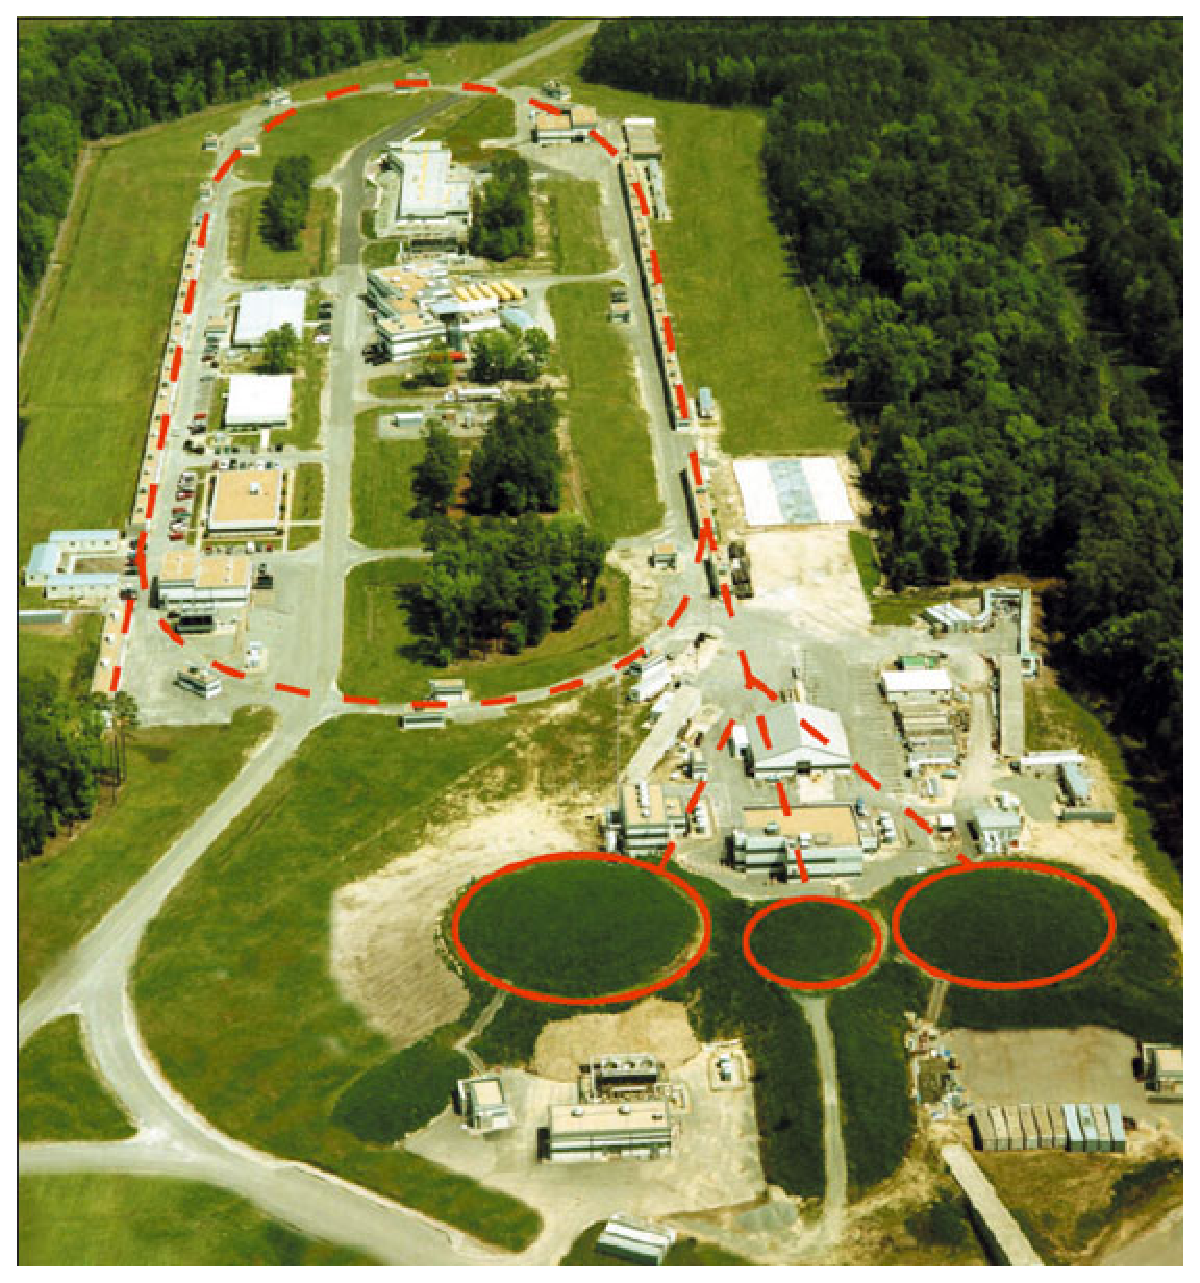
\includegraphics[width=1.0\columnwidth]{jlab}
%  \caption[Aerial view of Jefferson Lab \cite{jlab}.]{\label{fig:jlab}Aerial view of Jefferson Lab \cite{jlab}.}
%\end{center}
%\end{figure}
\setlength{\figwidth}{1.0\linewidth}
\Figure{jlab}{\figwidth}{Aerial view of Jefferson Lab \cite{jlab}.}

%\setlength{\figwidth}{0.9\linewidth}
%\Figure{cointime}{\figwidth}{cointime}

%
\Section{Accelerator}%
\label{Accelerator}
The length of the accelerator is about 7/8 of a mile for one complete cycle. A polarized electron source at the injector is used to extract electron beam of energy 45 MeV with the standard setup of JLab. The electron beam is accelerated by two linear accelerators, north and south linacs. A series of magnets bends the beam along the arcs which connects the two linacs. The beam line, transporting the beam to the three halls is shown in \figureref{beamline} by the RED lines. The continuous-wave (100\% duty factor) electron beam from the CEBAF accelerator has a characteristic 2 ns micro-structure that arises from the 1.5 GHz radio frequency (RF) structure of the accelerator and the 499 MHz three-hall beam splitting scheme. 

\SubSection{Polarized Source}%
\label{Polarized Source}
The production and acceleration of the electron beam starts with a polarized electron source. Circularly polarized light produces polarized electrons from a strained super-lattice gallium arsenide (GaAs) cathode through photoemission. This cathode is made up of several layers of material containing GaAs with varying amounts of phosphorus doping, grown on a substrate.

\SubSection{LINAC}%
\label{LINAC}
Electrons from the injector are sent to the north linear accelerator (linac) at an energy of 45 MeV. Superconducting niobium RF resonant cavities in the north linac section accelerate the electrons; in a standard tune, the maximum gain in energy per linac is 600 MeV in energy. The beam then goes through the east arc and into the south linac to be accelerated for another 600 MeV energy gain. This beam can be sent directly to the Beam Switch Yard (BSY) for distribution to the experimental halls or the beam can be steered along the west arc for another pass through the two linacs for another 1.2 GeV of energy gain. This process can be repeated up to four times. A maximum of five passes  through both linacs provide energies from 445 MeV to 5945 MeV. As the beam energies are different in each pass, a different set of magnets are used to steer the beam around the arcs after each pass.

\begin{figure}[!tbp]
  \centering
  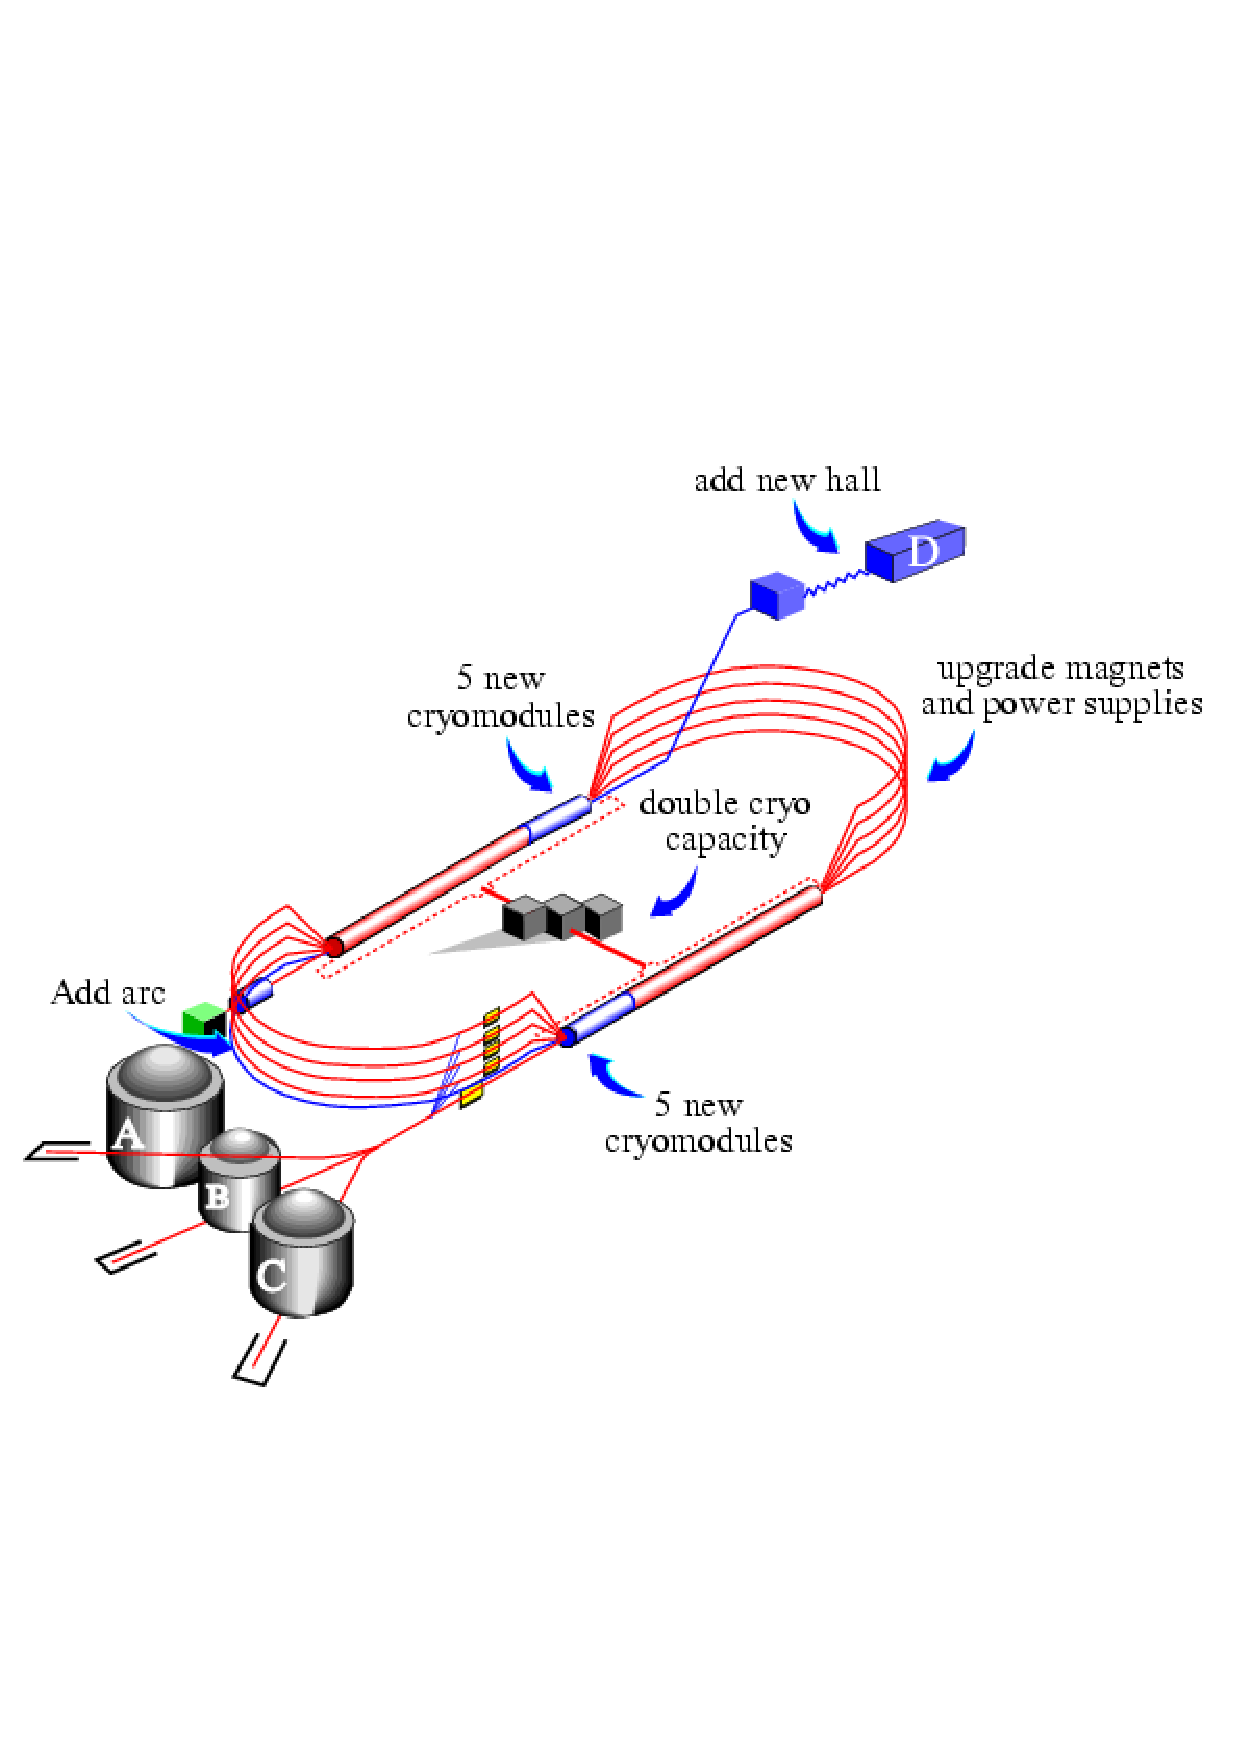
\includegraphics[trim = 0mm 57mm 0mm 50mm,clip,width=1.0\columnwidth]{beamline}
  \caption[Schematic of Jefferson Lab.]{\label{fig:beamline}Schematic of Jefferson Lab.\\\\ Beam is accelerated by two linear accelerator namely north linac and south linac. Three existing Halls A, B, C and one under construction, Hall-D, are shown. The new components that would be added for 12 GeV energy upgrade are also shown in the picture.}
\end{figure}
%\setlength{\figwidth}{0.9\linewidth}
%\Figure{beamline}{\figwidth}{Schematic of Jefferson Lab: Beam is accelerated by two linear accelerator namely north linac and south linac. Three existing Halls A, B, C and one under construction, Hall-D, are shown. The new components that would be added for 12 GeV energy upgrade are also shown in the picture.}
\Section{Beamline}%
\label{Beamline}
The beamlines that transport the beam from the accelerator to the experimental halls  is shown in \figureref{beamline}. Each beamline consists of a series of quadrupole and dipole magnets to help focus/ defocus the beam along the way to the target in each hall.

%Beamline of the Jefferson Lab has been shown in the \figureref{beamline}. The projected beamline of Hall-D and new cryogenic modules for 12 GeV upgradation are also shown in the figure. A series of powerful quadrupoles and dipoles are used along the beamline to focus and defocus the beam along the beamline. A two meter long dipole splits the beam for three diffrent halls.

\SubSection{Hall-C Beamline}
\label{Hall-C Beamline}
The beam position, profile and current were measured at various points along the Hall-C beamline. A part of Hall-C beamline also forms an arc. The bending magnets of the Hall-C arc can be used to measure the relative beam energy with a precision of $\Delta$E/E $\approx$ $10^{-4}$.

\SubSection{Beam Position Monitor}%
\label{Beam Position Monitor}
The beam position was continuously monitored by beam position monitors (BPM) during data collection to ensure that the beam was centered on the target. The transverse beam size was 60-130 $\mu$m in diameter and was measured by a superharp (pair of wires that can be moved in and out of the beam) scanner. The BPMs and superharps could measure the beam position with a precision of 0.2 $mm$ and 0.01 $mm$, respectively \cite{BC06}.

\SubSection{Beam Current Monitor}%
\label{Beam Current Monitor}
The beam current was monitored through a combination of a parametric DC current transformer (Unser monitor) and coupled cylindrical resonant cavities(Beam Current Monitor 1 and 2) which provided a continuous relative measurement of the current during each data run \cite{BC06,RM99}.

\SubSection{Raster}%
For liquid targets, the beam was rastered over an area of the target of up to 2x2 mm$^2$ by the Fast Raster to reach acceptable beam currents without damaging the target and to reduce the effect of localized boiling in the liquid targets.
%Slow raster was used to decrease the power density of the beam before the beam dump to reduce the damage.

\Section{Hall-C}%
\label{Hall-C}
The E01-107 experiment was performed in the Hall-C. Hall-C is shown in \figureref{HALC_33}. One can see the beamline is going to the target. There is a Short Orbit Spectrometer (SOS) on the left to collect scattered electrons and a High Momentum Spectrometer (HMS) to collect hadrons on the right at the far end. The unscattered beam is dumped in the Beam Dump at the other end of the hall. 
%The dimensions of the components can be realized by looking the scientist stnding on the left near Short Orbit Spectrometer hut.
%\begin{figure}[!tbp]
%  \centering
%  \includegraphics[width=1.0\columnwidth]{HALC_33}
%  \caption[Hall C at Jefferson Lab.]{\label{fig:HALC_33}Hall C at Jefferson Lab.}
%\end{figure}

\setlength{\figwidth}{1.0\linewidth}
\Figure{HALC_33}{\figwidth}{Hall C at Jefferson Lab.}

\SubSection{Short Orbit Spectrometer (SOS)}%
\label{SOS}
The Short Orbit Spectrometer uses three room temperature magnetic elements: a quadrupole followed by two dipoles (QDD) as shown in \figureref{sos} \cite{GaskelD}. The SOS can be rotated about the target in order to detect scattered particles at different scattering angles. In this experiment, scattered electron were detected in the SOS. The configuration of the detectors in the SOS is discussed in Section \ref{Detector Packages}.

\begin{figure}[tbp]
  \centering
  \includegraphics[trim = 0mm 4mm 2mm 0mm,clip,width=0.9\columnwidth]{sos}
  \caption[Side view of SOS \cite{GaskelD}.]{\label{fig:sos}Side view of SOS \cite{GaskelD}.}
\end{figure}
%\setlength{\figwidth}{0.8\linewidth}
%\Figure{sos}{\figwidth}{Side view of SOS \cite{GaskelD}.}

\SubSection{High Momentum Spectrometer (HMS)}%
\label{HMS}
The High Momentum Spectrometer is composed of four superconducting magnetic elements in order to focus and separate different particles based on their momentum and charge. In our experiment, $\pi^+$, $K^+$ and protons were detected in the HMS. The magnetic elements consisted of three quadrupoles followed by a dipole (QQQD) is shown in \figureref{hms} \cite{GaskelD}. The HMS can be rotated about the target as well. The configuration of the detectors in the HMS is discussed in Section \ref{Detector Packages}.

\begin{figure}[tbp]
  \centering
  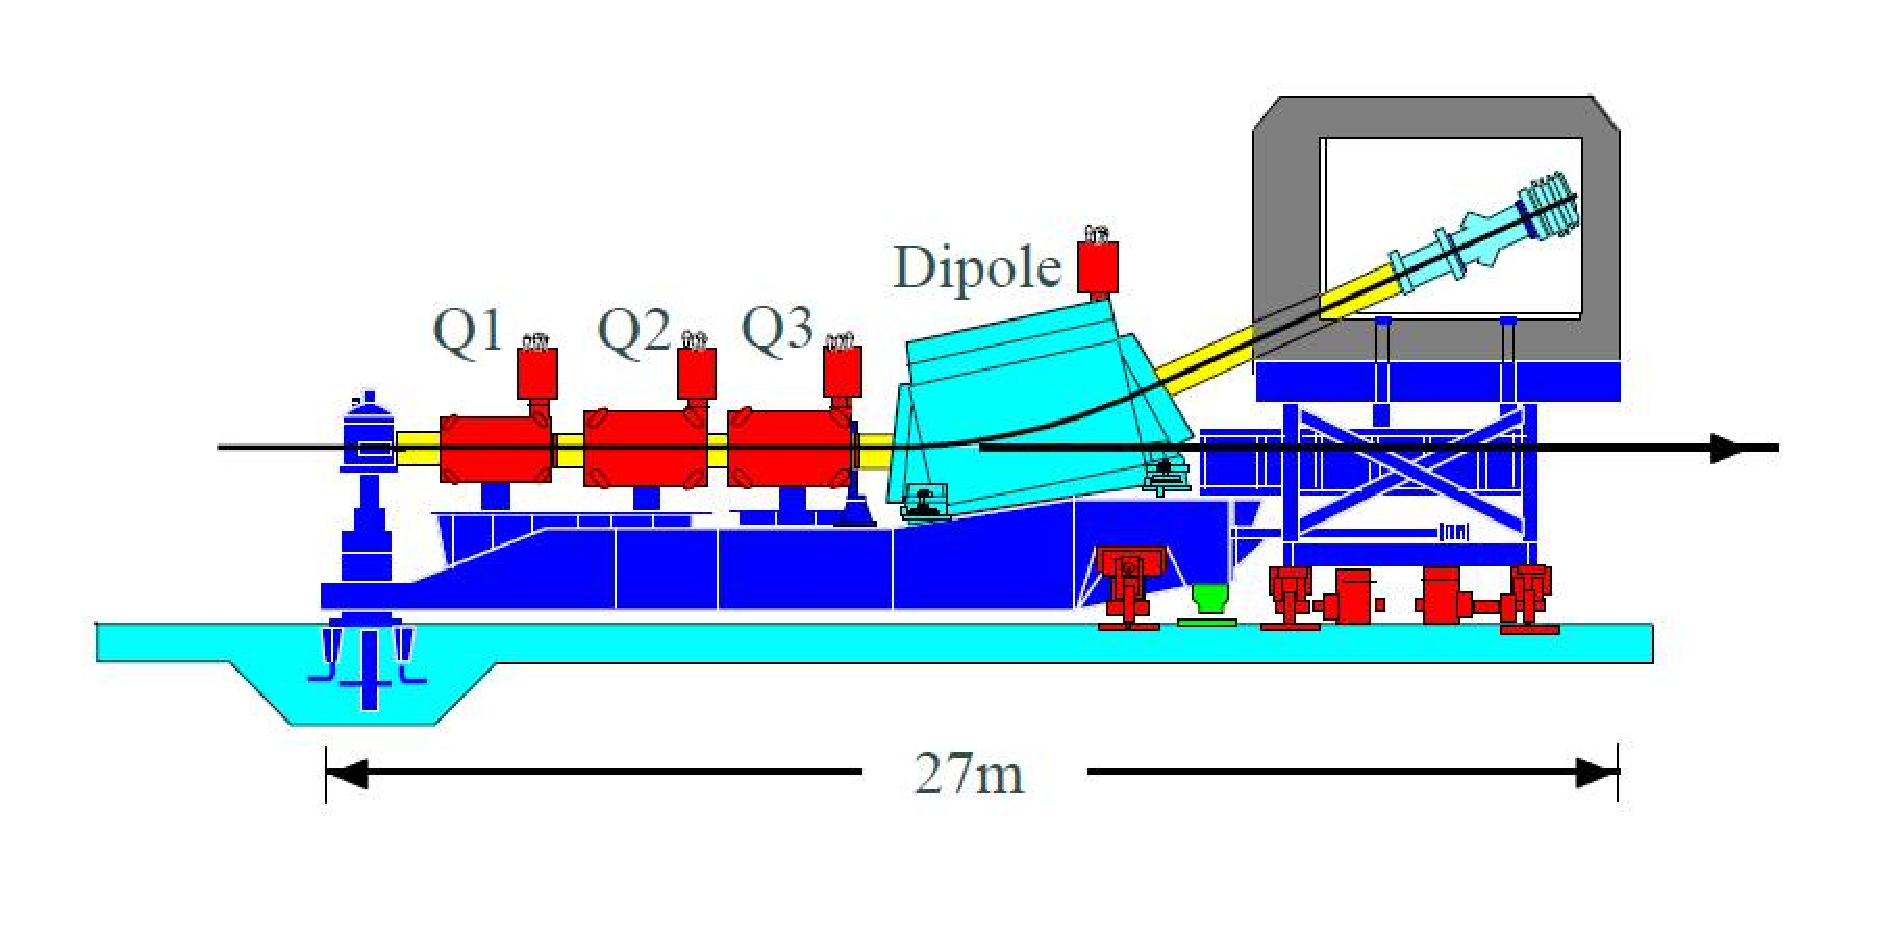
\includegraphics[trim = 0mm 10mm 2mm 0mm,clip,width=1.0\columnwidth]{hms}
  \caption[Side view of HMS \cite{GaskelD}.]{\label{fig:hms}Side view of HMS \cite{GaskelD}.}
\end{figure}
%\setlength{\figwidth}{1.0\linewidth}
%\Figure{hms}{\figwidth}{Side view of HMS \cite{GaskelD}.}

\SubSection{Target}%
\label{Target}
The electron beam with energy of up to 5.8 GeV was incident on liquid hydrogen and deuterium, and solid foil targets of $^{12}$C, $^{27}$Al, $^{63}$Cu, and $^{197}$Au. For the cryotargets, a 4.0 cm diameter cylindrical cell with an axis perpendicular to the beam direction was used. The cell walls with a thickness of 0.01 cm were made from an aluminum alloy. A schematic diagram of the cryogenic target ladder are shown in \figureref{target}. The target ladder could be translated vertically by lifter motors.

\begin{figure}[tbp]
  \centering
  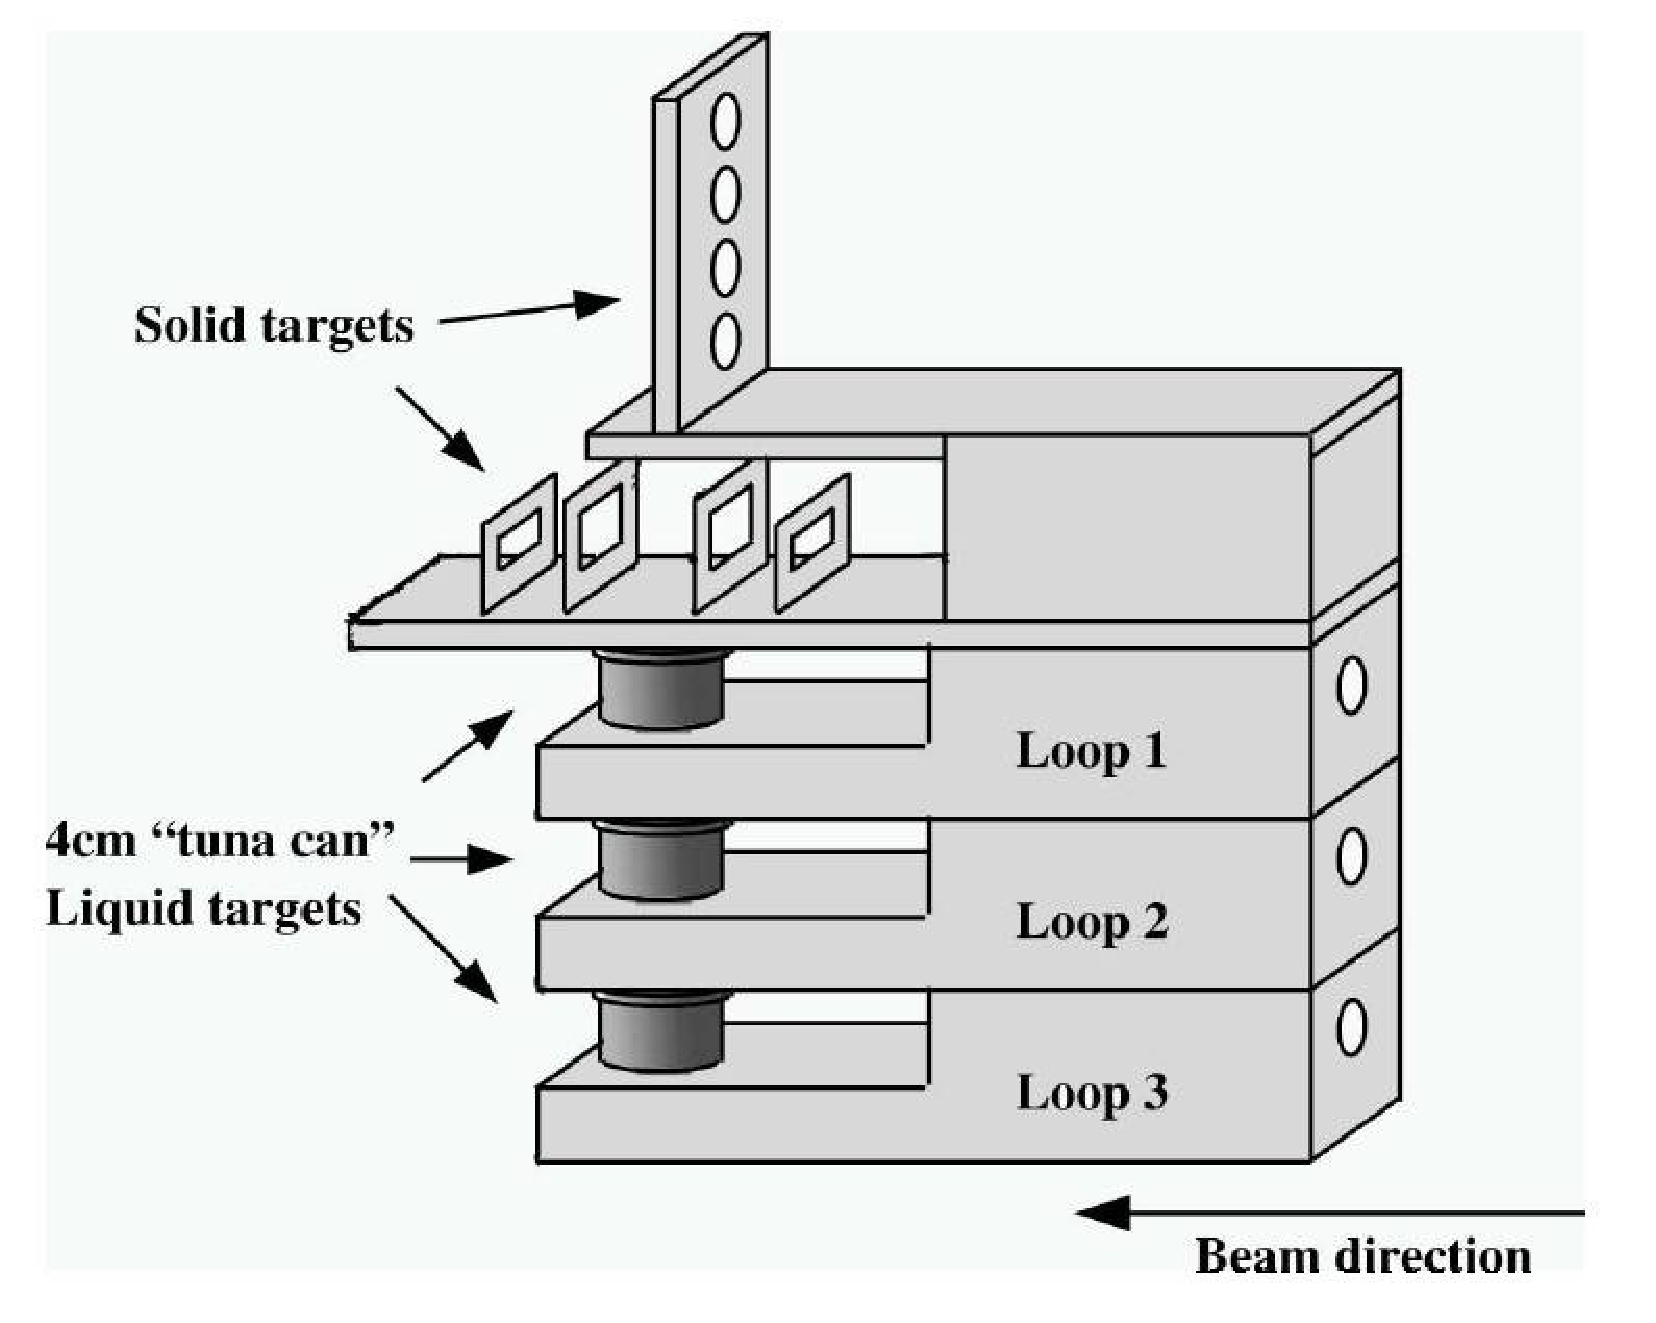
\includegraphics[width=0.8\columnwidth]{target}
  \caption[Schematic diagram of target ladder \cite{BC06}.]{\label{fig:target}Schematic diagram of target ladder \cite{BC06}.}
\end{figure}
%\setlength{\figwidth}{0.7\linewidth}
%\Figure{target}{\figwidth}{Schematic diagram of target ladder \cite{BC06}.}

\SubSection{Detector Packages}%
\label{Detector Packages}
There are two wire chambers each in the HMS and SOS, separated by 81.5 cm in the HMS and by 49.5 cm in the SOS to determine the position and angle of a track. Each wire chamber has six planes of wires and a 1:1 gas mixture of argon and ethane are surrounding the wires. The position resolutions of the HMS and SOS drift chambers were 280 $\mu$m and 180 $\mu$m, respectively \cite{BC06, hinton01}.

Four planes of scintillator hodoscopes are used both in the HMS and in the SOS to form the primary trigger for charged particle detection. These four planes were used to identify a particle that passed through them and produced signals.

$\breve{C}$erenkov detectors were used to detect the $\breve{C}$erenkov radiation emitted when a particle enters a medium and moves faster than the speed of light in that medium. Two types of $\breve{C}$erenkov detectors were used for particle identification (PID): Aerogel $\breve{C}$erenkov and Gas $\breve{C}$erenkov. Silica aerogel $\breve{C}$erenkov of refractive index n = 1.015 with threshold for $\pi^+$ of 0.8 GeV/c and a threshold for $K^+$ of 2.85 GeV/c was used; this allowed us to separate particles traveling above and below the threshold. A gas $\breve{C}$erenkov detector filled with 0.956 atm of perfluorobutane ($C_4F_{10}$) with an index of refraction of 1.0015 and a momentum threshold of 2.65 GeV/c for $\pi^+$ and threshold of 9.4 GeV/c for $K^+$ was used for PID as well \cite{BC06}.

%
\Section{Data Acquisition}%
\label{Data Acquisition}
The CEBAF Online Data Acquisition (CODA) software system managed real time reading of the data, its storage to disk as well as user interface \cite{Abb95}. Read Out Controller (ROC) CPUs managed the readout electronics, ADCs, TDCs and scalers. CODA software also read the ROCs directly via a parallel link over an ethernet network and wrote each event onto disk. Information about the beam position, magnet settings, target status and accelerator status were read out every 30 seconds using Experimental Physics Industrial Control System (EPICS) software \cite{RM99}.

%
\Section{Kinematic Settings}%
\label{Kinematic Settings}%
The E01-107 experiment was carried out in Hall C at Jefferson Lab \cite{CW01} in 2004. The kinematic settings of the measurements are shown in \Tableref{kine}. The experiment was designed to measure the nuclear transparency of pions using the ($e,e^\prime \pi^+$) reaction for five kinematic settings of $Q^2$ = 1.1, 2.15, 3.0, 3.91 and 4.69 $\mathrm{(GeV/c)^2}$. In addition to pions a reasonable sample of kaons were also recorded in the 30 ns coincidence window. The kaon statistics were very low for $Q^2$ = 3.91 and 4.69 $\mathrm{(GeV/c)^2}$ kinematic settings, hence this analysis covers only three kinematic settings, as listed in \Tableref{kine}.

More details of the experimental apparatus can be found in references \cite{BC06, RM99, hinton01}.

\begin{table}
  \caption[The central kinematics of the experiment.]{\label{tab:kine}The central kinematics of the experiment.}
\begin{center}
%\centering
\label{table1}
\begin{tabular}{||c|c|c|c|c|c|c|c||}\hline
 $Q^2$ & $-t$ & $E_e$ & $\theta_{e^\prime}^{\rm SOS}$ &$E_{e^\prime}$ &
 $\theta_{K^+}$ & $\theta_{\rm HMS}$ & $p_{K^+}$ \\
 (GeV/c)$^2$ & (GeV/c)$^2$ & GeV & deg & GeV & deg & deg & GeV/c \\\hline
1.10 &0.050 &4.021 &27.76 &1.190 &10.58 &10.61 &2.793 \\
2.15 &0.158 &5.012 &28.85 &1.730 &13.44 &13.44 &3.187 \\
3.00 &0.289 &5.012 &37.77 &1.430 &12.74 &12.74 &3.418 \\\hline
\end{tabular}
\vspace{-0.5cm}
\end{center}
\end{table}
%\Table{kine}{The central kinematics of the experiment.}


\chapter{Monte Carlo Simulation}
%chapsimc.tex
%
\Section{General Overview}%
%
In order to take into account the multi-dimensional phase space of the experiment, this analysis required a Monte Carlo simulation of the experiment to extract the yield of $K^+$s which is used to extract the nuclear transparency. The simulation uses a model of the electro-production of kaons from protons which includes multiple scattering, energy loss from passage through materials, kaon decay, and correction due to radiative processes.

The simulation code used for this analysis was based upon the code SIMULATE used by the SLAC NE-18 experiment \cite{PhysRevC.64.054610}. The code has been modified to include magnetic transport models of the spectrometer, HMS and SOS of Hall-C in Jefferson Lab and has been renamed as SIMC.

%
\Section{Ingredients of SIMC}%
%
\label{Ingredients of SIMC}
In this section we give an overview of some of the basic ingredients of SIMC.
%SIMC is the Monte Carlo simulation for Hall-C which have some basic ingradients. We are trying to give an overview of few ingradients in this section.

\SubSection{Event Generation}
\label{Event Generation}
The event generator for electron-proton scattering consists of randomly generated energy-momentum 4-vectors for all the initial and final particles within the constraints of energy-momentum conservation in a two-body reaction (the kaon-hyperon production is a two-body process). The incident electron 4-vector is generated from the known beam energy, randomly smeared by the energy resolution (0.1\%). The target proton 4-vector just requires the proton mass since it is at rest. The outgoing particles 4-vectors are generated within the allowed acceptance of the spectrometers. The event generation also randomly picks an interaction point that is within the length of the target and consistent with the beam raster amplitude used in the experiment. With this complete set of information on the interaction vertex, we can calculate the physics variables $Q^2$, $W$, $t$ and $\phi_{pq}$. Here $Q^2$ is four-momentum transferred square, $W$ is the C.M. energy, $t$ is the momentum transfer and $\phi_{pq}$ is  the angle between the scattering and reaction planes. The event generation is performed for the selected species of hyperons Y = ($\Lambda^0$, $\Sigma^0$, $\Sigma^-$).

%The simulation starts with randomly generated 4-vectors for the outgoing kaon and electron. The 4-vectors for the target proton are needed to solve the kinematics. The event generator first randomly choose a target interaction point which is consistent with the target length and raster amplitudes in the beam coordinate system. The beam energy of a resolution 0.5\% is selected with the given value in the input file. Then different quantities like $Q^2$, w, t, $\phi_{pq}$ etc. are randomly generated for each event. The Monte Carlo input file also species which hyperon Y = ($\Lambda$, $\Sigma^0$) is being generated for the kaon side reaction. Kaon hyperon production is a two body reaction and the momentum of the outgoing kaon in the center of mass frame is fixed by knowledge of w. The quantities $Q^2$, w, t and $\phi_{pq}$ are defined in the Section \ref{Comparison of Data with SIMC}.

\SubSection{Spectrometer Simulation}
\label{Spectrometer Simulation}
SIMC has realistic models of the magnetic spectrometers including multiple scattering and energy loss in all intervening material encountered by the particles. All outgoing particles are transported through the magnets to the detector huts by a set of matrix elements that model the passage of charged particles through the magnetic elements of the spectrometer. The position and angle (track) information, smeared by the wire-chamber resolution, at the focal plane of the spectrometer are calculated for all particles that make it through the detector elements. The smeared track at the focal plane is then reconstructed back to the target using another set of matrix elements. This mimics the method used to analyze the data.
%elements which are sequential for both the SOS and HMS. The focal plane quantities can be calculated based on a smeared wire chamber positions when the particles make through the detector elements. The required detector elements for the SOS is Cerenkov aerogel plane. Particle are being reconstructed at the target by using focal plane quantities. More about reconstructed quantities are discussed in the Section \ref{Comparison of Data with SIMC}

\SubSection{Physics Model}
\label{Physics Model}
The kaon electro-production from a proton is depicted in \figureref{reaction1}. A model of this reaction is in the simulation, SIMC. The five fold-differential cross section for this process can be expressed in terms of a photoproduction cross section $\frac{d^2\sigma}{d\Omega_K^*}$ multiplied by a virtual photon flux factor $\Gamma(Q^2, W)$. 
%The electroproduction cross section can then be written in terms of the scattered electron energy $E^\prime$ , electron lab frame solid angle $d\Omega_e^\prime = dSin\theta_e d\phi_e$ and kaon C.M solid angle $d\Omega_K^* = dSin\theta_{qK}^* d\phi$. The form of the virtual photoproduction cross section used for this analysis is
\begin{equation} \label{equ:model1}
\frac{d^5\sigma}{dQ^2dWd\phi_{e}d\Omega^*_K} = \Gamma(Q^2,W) \left(\frac{d^2\sigma}{d\Omega^*_K}\right)
\end{equation}

In the simulation, a transformation between ($Q^2$,W) $\leftrightarrow$ ($E^\prime$,$\Omega_e^\prime$) is incorporated into the virtual photon flux, where $E^\prime$ is energy of the scattered electron and $\Omega^\prime_e$ is electron lab frame solid angle, using

\begin{equation} \label{equ:model2}
\Gamma(Q^2,W) =  \Gamma_0(E^\prime,\Omega^\prime_e) \frac{W}{2m_pEE^\prime} = \frac{\alpha}{4\pi^2}  \frac{(W^2-m^2_p)}{2m^2_pE^2} \frac{W}{Q^2} \frac{1}{(1-\epsilon)}
\end{equation}

%\begin{figure}[!tbp]
%  \centering
%  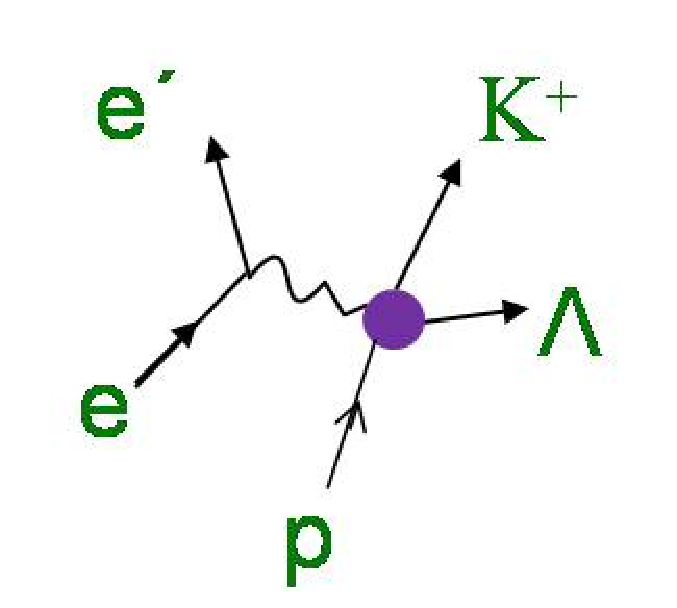
\includegraphics[width=0.4\columnwidth]{reaction1}
%  \caption[Schematic of kaon electro-production from proton.]{\label{fig:reaction1}Schematic of kaon electro-production from proton.}
%\end{figure}
\setlength{\figwidth}{0.4\linewidth}
\Figure{reaction1}{\figwidth}{Schematic of kaon electro-production from a proton.}
%In kaon transparency, the $K^+$ particle was detected in coincidence with the scattered electron, and therefore, the struck nucleon was constrained to be a proton by charge conservation. The struck proton was changed into a neutron by the interaction and a schematic of this process is shown in \figureref{reaction}.
\noindent
where $m_p$ is the mass of the proton and $\epsilon = \left(1 + \frac{2\left|\overline{q}\right|^2}{Q^2}\tan^2\frac{\theta_e}{2}\right)$ is the longitudinal polarization of the virtual photon.

The model for electro-production from nuclear targets schematically shown in \figureref{reaction2} was built from a parameterization of the measured cross section from a hydrogen target; for all other heavier targets (carbon, copper, gold) proton model is convoluted with a realistic spectral function for each target parametrized in terms of Eqs. \ref{equ:model1} and \ref{equ:model2}. Decay of kaons in flight and radiative corrections for all particles are also included in the model. 

\begin{figure}[!tbp]
  \centering
  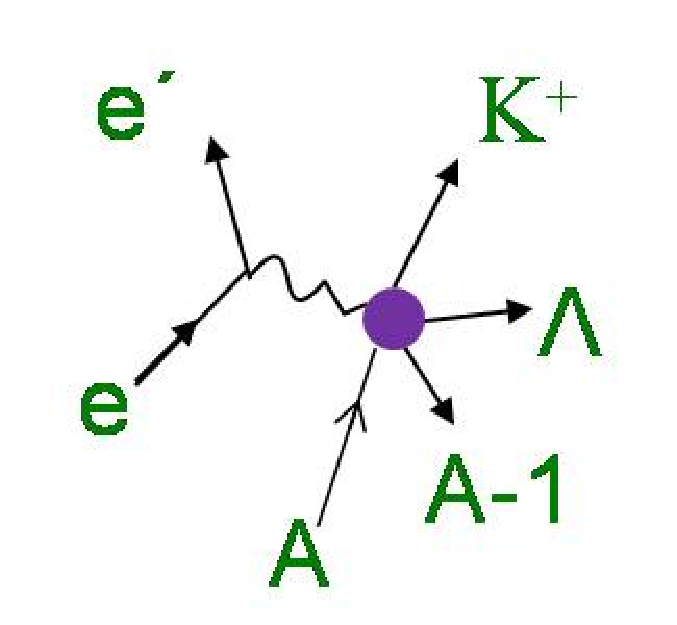
\includegraphics[width=0.4\columnwidth]{reaction2}
  \caption[Schematic of kaon electro-production from different targets.]{\label{fig:reaction2}Schematic of kaon electro-production from different targets.}
\end{figure}
%\setlength{\figwidth}{0.4\linewidth}
%\Figure{reaction2}{\figwidth}{Schematic of kaon electro-production from different targets.}

\SubSection{Kaon Decay}
\label{Kaon Decay}
In general, kaons are unstable and have a short mean lifetime which implies that a large fraction of the kaons which were created at the target decayed into secondary particles before they could be detected. The number of kaons that were actually detected was less than the true number of kaons produced in the reaction and corrections for their decay has been taken into account in the analysis ~\cite{RM99}. Kaon decay, multiple scattering, and energy loss are standard features in SIMC, and can be turned on and off using flags in the input files. Descriptions of corrections for these processes in the SIMC can be found in ~\cite{GaskelD}.

\SubSection{Spectral Function}
\label{Spectral Function}
The quasi-free model is used to describe electro-production from different nuclear targets used in the experiment. The incoming electron has larger energy compared to the binding energy of nucleons in the nucleus. So the bound nucleons in the target nucleus may be viewed as free nucleons. Properties of the nucleons inside of the nucleus are assumed to be described by an independent particle shell model, where each nucleon interacts with a mean field exerted by the other nucleons ~\cite{BC06}. The probability of finding a nucleon inside the nucleus with a certain energy and momentum can be defined by a spectral function. For heavier targets, the proton model is convoluted with a realistic spectral function for each target.

%
\Section{Comparison of Data with SIMC}%
%
\label{Comparison of Data with SIMC}
One of the goal of this analysis is to determine the normalized yields from the raw data collected during  the experiment. The normalized yield is the number of events that pass a given set of cuts divided by the cumulative charge delivered by the beam and corrected for the various inefficiencies of the experimental equipment. %Then transparency can be defined as the ratio of experimental yields from A $>$ 1 targets to hydrogen.
%
%\begin{equation} \label{equ:nucltransp1}
%T = 
%\frac{\bar Y_{\rm A}}{\bar Y_{\rm D}},
%\end{equation}
%
%$$T = \frac{Yield_A}{Yield_0}$$
%
%After comparing the data yields with SIMC yields, we have extracted nuclear transparency by forming a super ratio of the experimental yield to the Monte Carlo simulation yield, from nuclear targets and free protons (hydrogen), as shown in the expression below.
%
%\begin{equation} \label{equ:nucltransp3}
%T = 
%{\left( \frac{\bar Y}{\bar Y_{\rm MC}} \right)_A}/
%{\left( \frac{\bar Y}{\bar Y_{\rm MC}} \right)_{\rm D}},
%\end{equation}
%
%\begin{center}$$T=\frac{\frac{Yield_A^{data}}{Yield_A^{SIMC}}}{\frac{Yield_0^{data}}{Yield_0^{SIMC}}}$$\end{center}
%
%$\bar{Y}$ is the yield for data and $\bar{Y}_{MC}$ is for SIMC. A represent for the targets A$>$2 and D for Deuterium. The steps involved in extracting the normalized yields and transparency will be described in this chapter. Towards the goal of determining the nuclear transparency of kaons we have reconstructed the physical variables $Q^2$, W, t and $\phi_{pq}$ for each event at the interaction vertex. The measured yield is an integral over all of these variables.
%
%The cross section depends upon four variables, these are $Q^2$, W, t, $\phi_{pq}$. 

Before calculating the yields, we compare the data with SIMC yields, to verify that the Monte Carlo distributions agree with the measured distributions for these variables. If the shape of these distributions agree, it validates our model of kaon electro-production. The target quantities (horizontal slope $X_{tar}^\prime$, vertical slope $Y_{tar}^\prime$ and the momentum fraction of the particle with respect to the spectrometer central momentum $\delta$) were reconstructed using the focal plane quantities $X_{fp}$(horizontal position), $X_{fp}^\prime$ (horizontal angle), $Y_{fp}$ (vertical position) and $Y_{fp}^\prime$ (vertical position) on the focal plane\footnote{Focal plane is perpendicular to the central ray.} for HMS and SOS. The reconstructed angle and momentum fraction at the target are labeled as \textit{hsxptar}, \textit{hsyptar} and \textit{hsdelta} for the HMS and \textit{ssxptar}, \textit{ssyptar} and \textit{ssdelta} for the SOS.

%\setlength{\figwidth}{0.8\linewidth}
%\Figure{com_plot_Q2_2}{\figwidth}{$Q^2$. Clockwise from top left corener: $Q^2_\Lambda$ SIMC, $Q^2_\Sigma$ SIMC, $Q^2_\Sigma$ data, $Q^2_\Lambda$ data}

%\setlength{\figwidth}{1.0\linewidth}
%\Figure{Q2_2}{\figwidth}{$Q^2$ combined $\Lambda$ and $\Sigma$ for both SIMC and data}

%\setlength{\figwidth}{0.8\linewidth}
%\Figure{com_plot_w_2}{\figwidth}{W. Clockwise from top left corener: $W_\Lambda$ SIMC, $W_\Sigma$ SIMC, $W_\Sigma$ data, $W_\Lambda$ data}

%\setlength{\figwidth}{0.8\linewidth}
%\Figure{w_2}{\figwidth}{W combined $\Lambda$ and $\Sigma$ for both SIMC and data}

%\setlength{\figwidth}{0.8\linewidth}
%\Figure{com_plot_t_2}{\figwidth}{t. Clockwise from top left corener: $t_\Lambda$ SIMC, $t_\Sigma$ SIMC, $t_\Sigma$ data, $t_\Lambda$ data}

%\setlength{\figwidth}{0.8\linewidth}
%\Figure{t_2}{\figwidth}{t combined $\Lambda$ and $\Sigma$ for both SIMC and data}

%\setlength{\figwidth}{0.8\linewidth}
%\Figure{com_plot_phi_2}{\figwidth}{$\phi^{pq}$. Clockwise from top left corener: $\phi^{pq}_\Lambda$ SIMC, $\phi^{pq}_\Sigma$ SIMC, $\phi^{pq}_\Sigma$ data, $\phi^{pq}_\Lambda$ data}

%\setlength{\figwidth}{0.8\linewidth}
%\Figure{phipq_2}{\figwidth}{$\phi^{pq}$ combined $\Lambda$ and $\Sigma$ for both SIMC and data}

Beside applying cuts on $Q^2$, $W$, $t$ and $\phi_{pq}$, cuts were applied on these reconstructed quantities (such as \textit{hsxptar}, \textit{ssxptar}, \textit{hsyptar}, \textit{ssyptar}, \textit{hsdelta} and \textit{ssdelta}) both on the data and SIMC yields, as they define the feducial acceptance of the detector. In order to restrict the data to regions where they match the simulation, we applied very tight cuts on these fiducial acceptances. The cuts are discussed in Section~\ref{Cuts}.

%\setlength{\figwidth}{0.8\linewidth}
%\Figure{com_plot_2_ptar_2}{\figwidth}{Clockwise from top left corener: hsxptar, ssxptar, ssyptar and hsyptar. \textcolor{red}{RED} shows for SIMC and \textcolor{blue}{BLUE} shows for data}
%\setlength{\figwidth}{0.8\linewidth}
%\Figure{com_plot_sxptar_2}{\figwidth}{Clockwise from top left corener: $hsxptar_\Lambda$, $hsxptar_\Sigma$, $ssxptar_\Sigma$ and $ssxptar_\Lambda$. \textcolor{red}{RED} shows for SIMC and \textcolor{blue}{BLUE} shows for data}
\begin{figure}[!tbp]
  \centering
  \includegraphics[width=0.8\columnwidth]{com_plot_2_hms_2}
  \caption[HMS reconstructed angles and momentum fraction.]{\label{fig:com_plot_2_hms_2}HMS reconstructed angles and momentum fraction.\\\\ $hsxptar$, $hsyptar$, $hsytar$ and $hsdelta$ for $\Lambda$ production of $K^+$ after applying cuts on the variables. RED for SIMC and BLUE for data.}
\end{figure}
%\setlength{\figwidth}{0.8\linewidth}
%\Figure{com_plot_2_hms_2}{\figwidth}{HMS reconstructed angles and momentum fraction (hsxptar, hsyptar, hsytar and hsdelta) for $\Lambda$ production of $K^+$ after applying cuts on the variables. \textcolor{red}{RED} for SIMC and \textcolor{blue}{BLUE} for data.}

\begin{figure}[!tbp]
  \centering
  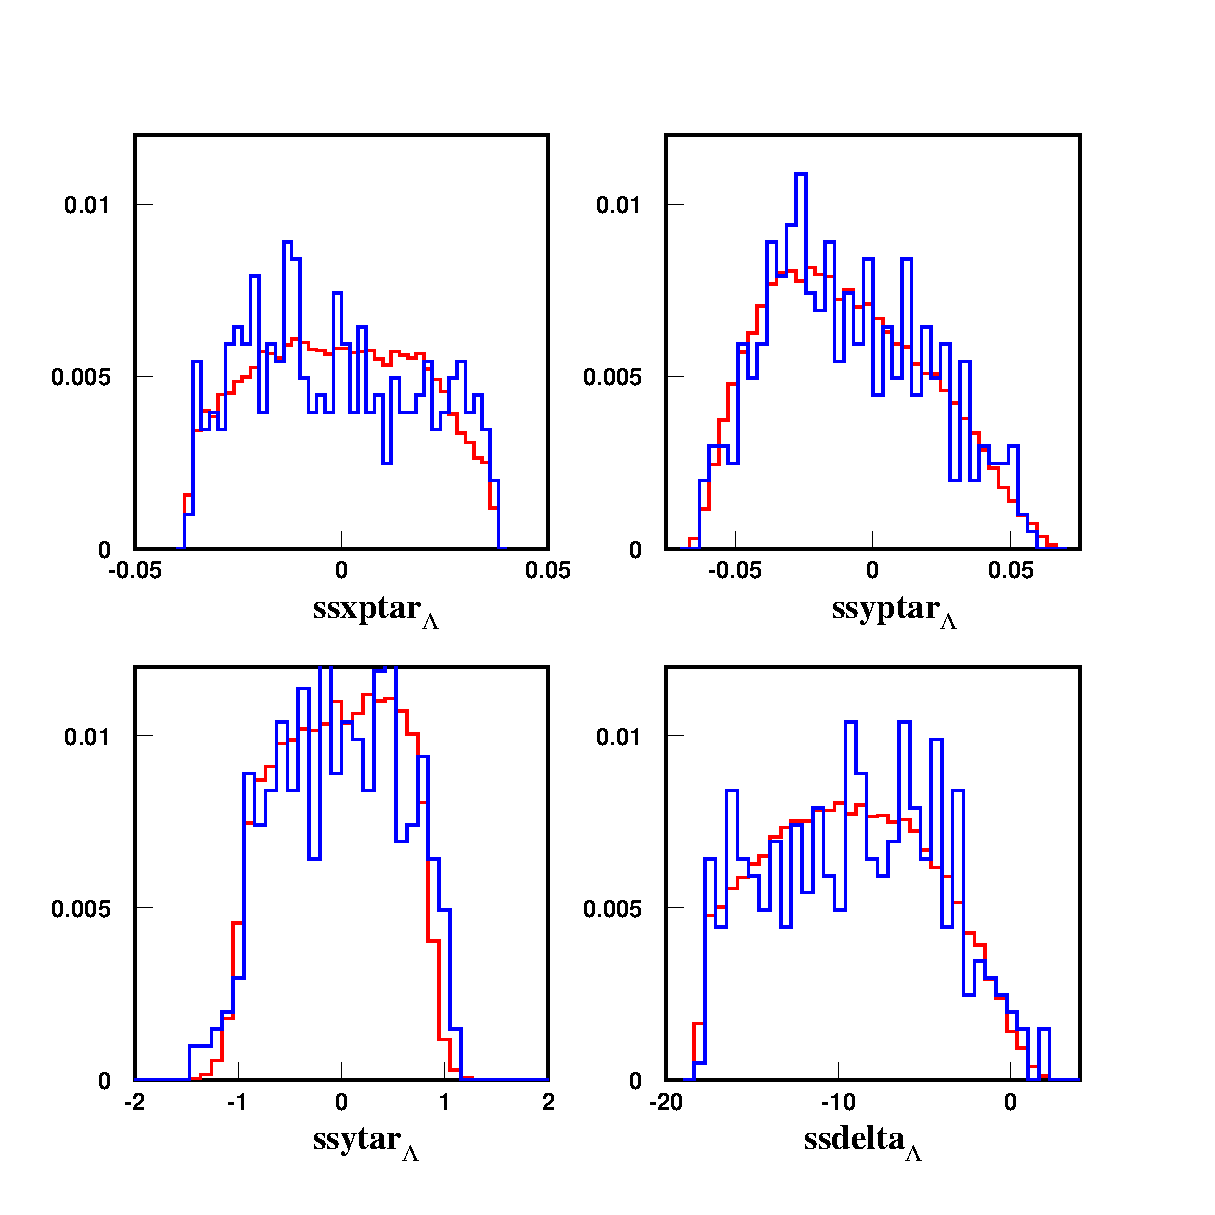
\includegraphics[width=0.8\columnwidth]{com_plot_2_sos_2}
  \caption[SOS reconstructed angles and momentum fraction.]{\label{fig:com_plot_2_sos_2}SOS reconstructed angles and momentum fraction.\\\\ $ssxptar$, $ssyptar$, $ssytar$ and $ssdelta$ for $\Lambda$ production of $K^+$ after applying cuts on the variables. RED for SIMC and BLUE for data.}
\end{figure}
%\setlength{\figwidth}{0.8\linewidth}
%\Figure{com_plot_2_sos_2}{\figwidth}{SOS reconstructed angles and momentum fraction (ssxptar, ssyptar, ssytar and ssdelta) for $\Lambda$ production of $K^+$ after applying cuts on the variables. \textcolor{red}{RED} for SIMC and \textcolor{blue}{BLUE} for data.}

As a representative sample, we have shown the comparison of data with SIMC yields for the reconstructed target variables in the case of $\Lambda$ production at $Q^2$ = 2.2 $\mathrm{(GeV/c)^2}$. BLUE and RED show data and SIMC, respectively, for the HMS in \figureref{com_plot_2_hms_2} and for the SOS in \figureref{com_plot_2_sos_2}. Similarly comparisons were also performed for $\Lambda$ and $\Sigma$ production at $Q^2$ = 1.1 to 3.0 $\mathrm{(GeV/c)^2}$, but are not shown here.

%Cuts on these feducial acceptances are being shown in the \figureref{com_plot_2_hms_2} and \figureref{com_plot_2_sos_2}. We have compared data with SIMC for the reconstructed target variables in case of $\Lambda$ production of kinematics $Q^2$ = 2.2 $(GeV/c)^2$ shown by \textcolor{blue}{BLUE} and \textcolor{red}{RED} respectively for HMS in the \figureref{com_plot_2_hms_2}. Same has been shown for SOS in the \figureref{com_plot_2_sos_2}. Similarly we applied for $\Sigma$ production for this kinematics and considered other kinematics of $Q^2$ = 1.1, 3.0 $(GeV/c)^2$ as well.

\chapter{Analysis}
%chapanalysis.tex
%
\Section{General Overview}%
%
One of the goals of the analysis is to determine the normalized yields from the raw data collected during the experiment. The normalized yield is the number of events that pass a given set of cuts divided by the cumulative charge delivered by the beam and corrected for various inefficiencies of the experimental equipment. We have extracted nuclear transparency by forming a super ratio of the experimental yield to the Monte Carlo simulation yield from given targets with nucleon number $A$ and deuterium. This ratio is shown in the expression below:

\begin{equation} \label{equ:nucltransp}
T = 
{\left( \frac{\bar Y}{\bar Y_{\rm MC}} \right)_A}/
{\left( \frac{\bar Y}{\bar Y_{\rm MC}} \right)_{\rm D}},
\end{equation}

%\begin{center}$$T=\frac{\frac{Yield_A^{data}}{Yield_A^{SIMC}}}{\frac{Yield_0^{data}}{Yield_0^{SIMC}}}$$
%\end{center}

$\bar{Y}$ is experimental charge-normalized data yield and $\bar{Y}_{MC}$ is the charge-normalized Monte Carlo equivalent yield. In this chapter, we will describe the steps involved in extracting the normalized yields and transparency. For determining the nuclear transparency of kaons, we have reconstructed the physical variables $Q^2$, $W$, $t$ and $\phi_{pq}$ for each event at the interaction vertex.
%Where $Q^2$ is four momentum transfered square, W is the center of mass energy, t is momentum transfer in the center of mass frame and $\phi_{pq}$ is  the angle between the scatering and reaction planes.
The measured yield is an integral over all of these variables.

\Section{Particle Identification(PID)}%
%
\label{Particle Identification(PID)}
We have used particle track information from drift chambers, time-of-flight information from scintillators, response from a gas $\breve{C}$erenkov detector and an aerogel $\breve{C}$erenkov detector to identify the kaons and separate them from other hadrons, such as pions and protons.

\SubSection{Tracking}%
The drift chambers provide the position, angle and momentum (relative to the central momentum) of the particles passing through the spectrometer. We have applied cuts on the reconstructed position, angle and momentum to ensure that they are well within the spectrometer acceptance. Due to poor statistics at the edges of the acceptance, tight cuts were applied on these variables to ensure a good match between the data and SIMC yields.

\SubSection{Charge-Normalized Yield}%
The charge normalized yield can be defined as 
\begin{equation}
\bar{Y} = \frac{Y}{Q}
\end{equation}
where $Y$ is the yield of a given run in counts and $Q$ is the charge delivered by beam (in mC), measured by Beam Current Monitors (BCM) and integrated over the time duration of a run. The yield is given by

\begin{equation} \label{equ:yield}
Y = \frac{N_{true}}{[\epsilon_{scer}\epsilon_{track}f_{elec}]_{SOS}[\epsilon_{hcer}\epsilon_{haero}\epsilon_{track}/f_{elec}]_{HMS}}\frac{N_{pretrigger}}{N_{trigger}}\frac{1}{T_h}
\end{equation}

\noindent
where $N_{true}$ is the true number of events, $f_{elec}$ is electronic dead-time correction factor, $\epsilon_{hcre}$ is the HMS $\breve{C}$erenkov efficiency, $\epsilon_{scre}$ is the SOS $\breve{C}$erenkov efficiency, $\epsilon_{aero}$ is the HMS aerogel efficiency, $\epsilon_{track}$ is the HMS/SOS tracking efficiency and $\frac{N_{trigger}}{N_{pretrigger}}$ is the lifetime. The transmission through the target material, the window of the scattering chamber, the windows of the spectrometer, etc. are collectively referred to as $T_h$.

\SubSection{Coincidence Time}%
Coincidence time is defined as the difference of the time taken by the scattered electrons to reach the SOS to the time taken by the hadrons (p, $\pi^+$, $K^+$) to reach the HMS. Good coincidence timing is the most useful and important information used to achieve clean real $K^+$ yield and helps to measure the insufficiencies of the most of the other cuts.

\begin{figure}[!tbp]
  \centering
  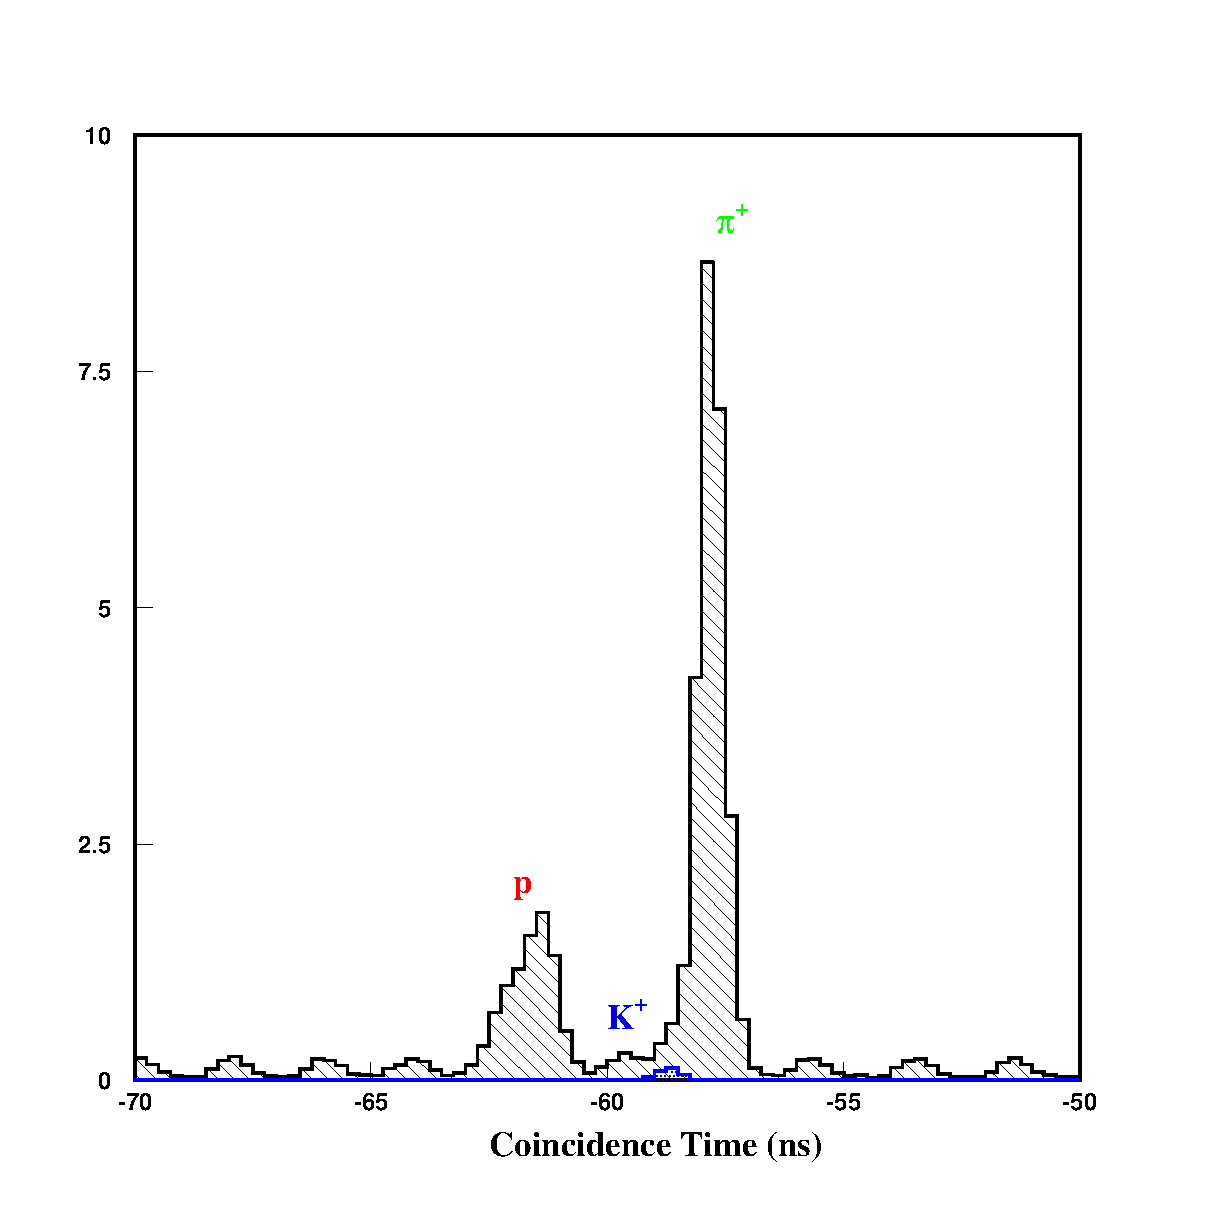
\includegraphics[trim = 1mm 1mm 1mm 1mm,clip,width=0.8\columnwidth]{cointime1}
  \caption[Coincidence time plot of the experiment.]{\label{fig:cointime1}Coincidence time plot of the experiment.\\\\ The broad peak in the right side is from $\pi^+$, proton peak in the left and reasonable number of $K^+$ in the middle shown in BLUE.}
\end{figure}
%\setlength{\figwidth}{0.8\linewidth}
%\Figure{cointime1}{\figwidth}{Coincidence time plot of the experiment. The broad peak in the right side is from $\pi^+$, proton peak in the left and reasonable number of $K^+$ in the middle shown in \textcolor{blue}{BLUE}.}

\begin{figure}[!tbp]
  \centering
  \includegraphics[trim = 1mm 1mm 1mm 1mm,clip,width=0.8\columnwidth]{cointime2}
  \caption[Zoomed coincidence time plot of the experiment.]{\label{fig:cointime2}Zoomed coincidence time plot of the experiment.\\\\ The selected peak of $K^+$ in BLUE in the middle from $\pi^+$ and proton peak in the right and left, respectively, after applying all the cuts.}
\end{figure}
%\setlength{\figwidth}{0.8\linewidth}
%\Figure{cointime2}{\figwidth}{Zoomed coincidence time plot of the experiment. The selected peak of $K^+$ in \textcolor{blue}{BLUE} in the middle from $\pi^+$ and proton peak in the right and left, respectively, after applying all the cuts.}

The time-of-flights (TOF) of the electron in the SOS and of hadrons in the HMS were obtained from the TOF scintillator detectors in each spectrometer. These were used to determine the coincidence time, which is the relative time difference between the electron and the hadron projected back to the target. Cuts on coincidence time were used to separate kaons from pions and protons.

A typical plot of the coincidence time of the experiment is shown in \figureref{cointime1}. Since the experiment was designed for pions, one can see a sharp peak of $\pi^+$ in the 30 ns coincidence window. There is a broad peak of protons as well and between protons and $\pi^+$ peak there is a rather small peak of kaons. In \Figureref{cointime1}, the small periodic peaks at an interval of 2.004 ns are due to the 499 MHz pulse structure of the beam delivered by the accelerator to Hall-C. One of the most effective PID cuts was over coincidence time in order to separate $K^+$ from $\pi^+$ and protons. Selected kaons after applying all the cuts are shown by BLUE region in \Figureref{cointime2}.

The fraction of electron-kaon coincidences that were uncorrelated accidental coincidences must be corrected in order to arrive at the true electro-production yield. The accidental coincidences have been corrected using the average number of kaon events in three of the small peaks that are 2.004 ns apart on both sides of the central coincidence time peak and has been shown by the GREEN band in \figureref{misscoin}.

\SubSection{Missing Mass}%
\label{Missing Mass}
To understand missing mass, we need to look into the basic reactions of the experiment, which can 
be written as
\begin{equation}
\label{L0}
e + p \rightarrow e^\prime + K^+ + \Lambda^0
\end{equation}
\begin{equation}
\label{S0}
e + p \rightarrow e^\prime + K^+ + \Sigma^0
\end{equation}
\begin{equation}
\label{S-}
e + n \rightarrow e^\prime + K^+ + \Sigma^-
\end{equation}
In the nucleus, the reaction can be written as
\begin{equation}
e + A \rightarrow e^\prime + K^+ + \Lambda^0 + X
\end{equation}
\begin{equation}
e + A \rightarrow e^\prime + K^+ + \Sigma^0 + X
\end{equation}
\begin{equation}
e + A \rightarrow e^\prime + K^+ + \Sigma^- + X
\end{equation}
Since the $\Lambda$/$\Sigma$ are not detected, from energy and momentum conservation we can write from Eq. \ref{L0}, \ref{S0} and \ref{S-},\\
Energy conservation: 
\begin{equation}
E_e + M_p = E_{e^\prime} + E_{K^+} + E_X ~\mathrm{or,}~ E_X = E_e + M_p - E_{e^\prime} - E_{K^+}
\end{equation}
Momentum conservation:
\begin{equation}
P_e + 0 = P_{e^\prime} + P_{K^+} + P_X ~\mathrm{or,}~ P_X = P_e + 0 - P_{e^\prime} - P_{K^+}
\end{equation}

Then we can form a variable called missing mass as 
\begin{equation}
M_X =  \sqrt{E_X^2 - P_X^2 }
\end{equation}

Those events which have a missing mass equal to the  $\Lambda^0$ particle can be identified as being produced in the e + p $\rightarrow$ $e^\prime$ + $K^+$ + $\Lambda^0$ reaction. By placing a cut on $M_X$ around $M_{\Lambda^0}$, we can choose those $K^+$ produced in the first reaction shown above. Similarly, by cutting on the missing mass around the $\Sigma^0$ and $\Sigma^-$ mass, we can select the $K^+$ produced from the second and third reactions, respectively.
%Basically, if the missing mass turns to be the mass of the particle $\Lambda$ particle then the $\Lambda$ channel reaction occured and $K^+$ produced during the reaction. For example giving a cut over $M_\Lambda$ we can choose those $K^+$ produced in the first reaction.
%Similarly, we can form the missingmass $M_\Sigma$ and $M_\Sigma^-$ variable for $\Sigma^0$ and $\Sigma^-$ production.\\

The basic idea is to use the reconstructed missing mass and cuts around the various hyperons masses to separate $K^+$ from p and $\pi^+$ as well as to separate the $\Lambda$ from $\Sigma^0$ and $\Sigma^-$ production of $K^+$ from protons. As the statistics were very low, it was very difficult to separate $\Sigma^0$ and $\Sigma^-$ for the events. We did not try to distinguish between the production of $\Sigma^0$ and $\Sigma^-$. More details follow in Section \ref{Transparency}.

\begin{figure}[!tbp]
  \centering
  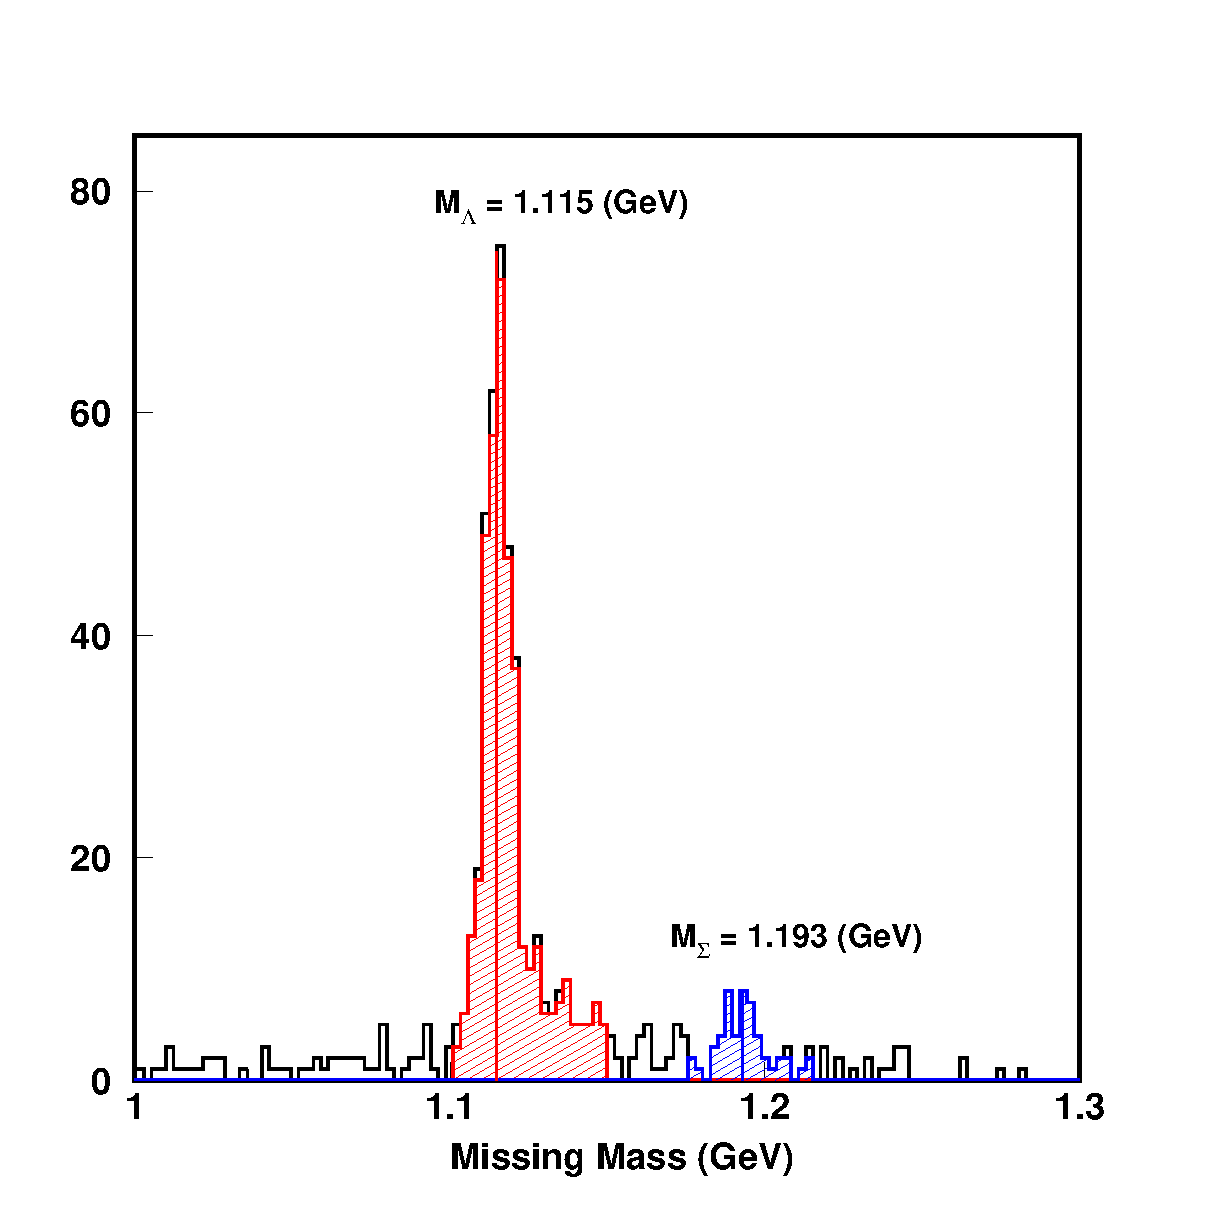
\includegraphics[width=0.8\columnwidth]{missmass1}
  \caption[One-dimensional missing mass plot.]{\label{fig:missmass1}One-dimensional missing mass plot.\\\\ First sharp peak is due to $\Lambda$ production and second small peak is due to $\Sigma$ production of kaons.}
\end{figure}
%\setlength{\figwidth}{0.8\linewidth}
%\Figure{missmass1}{\figwidth}{One-dimensional missing mass plot. First sharp peak is due to $\Lambda$ and second small peak is due to $\Sigma^0$.}

%\setlength{\figwidth}{1.0\linewidth}
%\Figure{missmass2}{\figwidth}{One dimensional plot of missing mass are shown here after applying cuts. Clockwise top left corner: $M_\Lambda^{SIMC}$, $M_\Sigma^{SIMC}$, $M_\Sigma^{data}$ and $M_\Lambda^{data}$}

\begin{figure}[!tbp]
  \centering
  \includegraphics[width=0.8\columnwidth]{com_plot_missmass_2}
  \caption[One-dimensional missing mass plot after applying cuts.]{\label{fig:com_plot_missmass_2}One-dimensional missing mass plot after applying cuts.\\\\ $M_\Lambda^{SIMC}$ and $M_\Sigma^{SIMC}$ are shown in RED and $M_\Sigma^{data}$ and $M_\Lambda^{data}$ are in BLUE.}
\end{figure}
%\setlength{\figwidth}{0.8\linewidth}
%\Figure{com_plot_missmass_2}{\figwidth}{One-dimensional plot of missing mass is shown here after applying cuts. $M_\Lambda^{SIMC}$ and $M_\Sigma^{SIMC}$ are shown in \textcolor{red}{RED} and $M_\Sigma^{data}$ and $M_\Lambda^{data}$ are in \textcolor{blue}{BLUE}.}

\begin{figure}[!tbp]
  \centering
  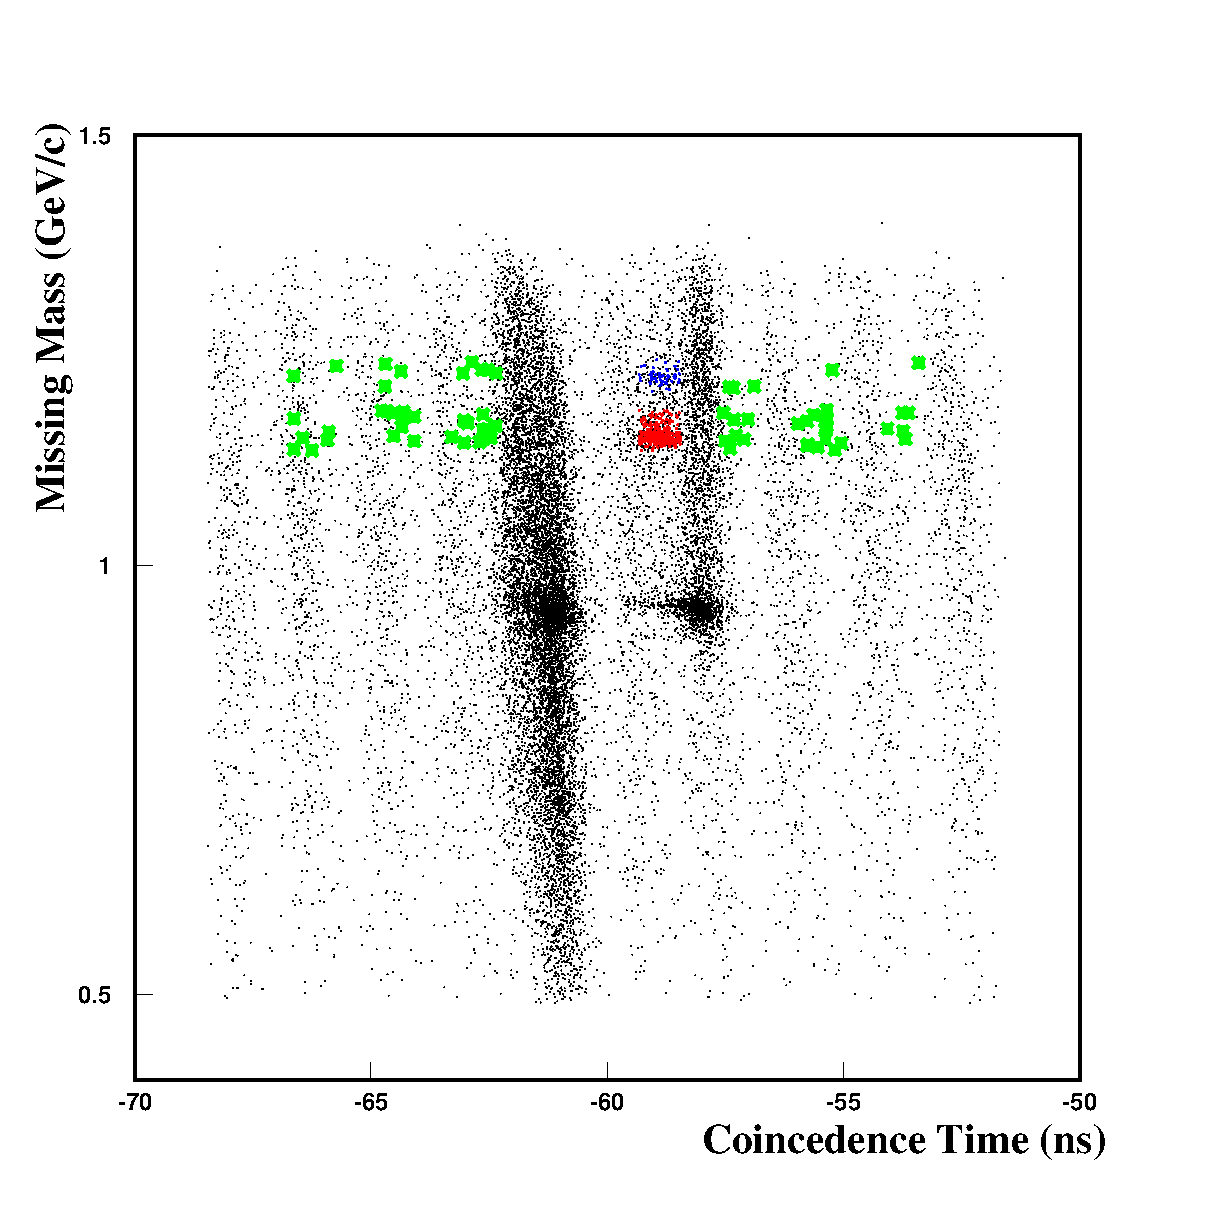
\includegraphics[trim = 3mm 3mm 3mm 3mm,clip,width=0.8\columnwidth]{misscoin}
  \caption[Two-dimensional plot of missing mass vs coincidence time.]{\label{fig:misscoin}Two-dimensional plot of missing mass vs coincidence time.\\\\ p, $K^+$ and $\pi^+$ are shown here from left to right, respectively, after applying loose cuts.}
\end{figure}
%\setlength{\figwidth}{0.8\linewidth}
%\Figure{misscoin}{\figwidth}{Two-dimensional plot of missing mass vs coincidence time. p, $K^+$ and $\pi^+$ are shown here from left to right, respectively, after applying loose cuts.}

Using the missing mass variable for hydrogen data, we have separated $K^+$ from $\Lambda$ and $\Sigma$ production. From these events, we determine a ratio of $\frac{\Lambda}{\Sigma}$.We used this same ratio in the Monte Carlo simulation. In targets heavier than hydrogen, the Fermi motion\footnote{The quantum motion of nucleons bound inside a nucleus is knwon as Fermi motion.} of the nucleons begin to broaden the $\Lambda$ and $\Sigma$ peak and are very difficult to distinguish. For all other targets due to the spreading of $\Lambda$ and $\Sigma$, we used a single cut over both $\Lambda$ and $\Sigma$ masses to separate $K^+$.

The missing mass spectrum shown in \figureref{missmass1} is from the hydrogen target for $Q^2$ = 1.1 $(\mathrm{GeV/c})^2$. In \figureref{missmass1}, the BLACK region represents events without any cut and the RED region represents the application of the cut on missing mass for $K^+$ production from $\Lambda$ and BLUE shows from the $\Sigma$ channel, whereas the RED vertical line at $M_\Lambda$ = 1.115 $(\mathrm{GeV/c})^2$ shows the mass of $\Lambda$ and BLUE vertical line at $M_\Sigma$ = 1.193 $(\mathrm{GeV/c})^2$ shows the mass of $\Sigma$ from \cite{PDG}. For $\Sigma$ mass we have taken average of the mass of $\Sigma^0$ and $\Sigma^-$ since we have two $\Sigma$ channels; given our meagre statistics, we are unable to separate $\Sigma^0$ and $\Sigma^-$ productions.

The missing mass variable is shown in \figureref{com_plot_missmass_2} after applying all the cuts where the SIMC yields are shown by RED and data by BLUE. $\Lambda$ and $\Sigma$ production have been separated by using the hydrogen data. \figureref{misscoin} shows two-dimensional plot of missing mass vs coincidence time. The $\Lambda$ events are shown in RED and $\Sigma$ in BLUE.

\begin{figure}[!tbp]
  \centering
  \includegraphics[width=0.8\columnwidth]{pid1}
  \caption[Aerogel $\breve{C}$erenkov detector.]{\label{fig:pid1}Aerogel $\breve{C}$erenkov detector.\\\\ Proton, pion and kaon thresholds for producing $\breve{C}$erenkov radiation in the aerogel $\breve{C}$erenkov detector are shown by RED, GREEN and BLUE curves respectively.}
\end{figure}
%\setlength{\figwidth}{0.8\linewidth}
%\Figure{pid1}{\figwidth}{Aerogel $\breve{C}$erenkov detector: Proton, pion and kaon thresholds for producing $\breve{C}$erenkov radiation in the aerogel $\breve{C}$erenkov detector are shown by \textcolor{red}{RED}, \textcolor{green}{GREEN} and \textcolor{blue}{BLUE} curves respectively.}

\begin{figure}[!tbp]
  \centering
  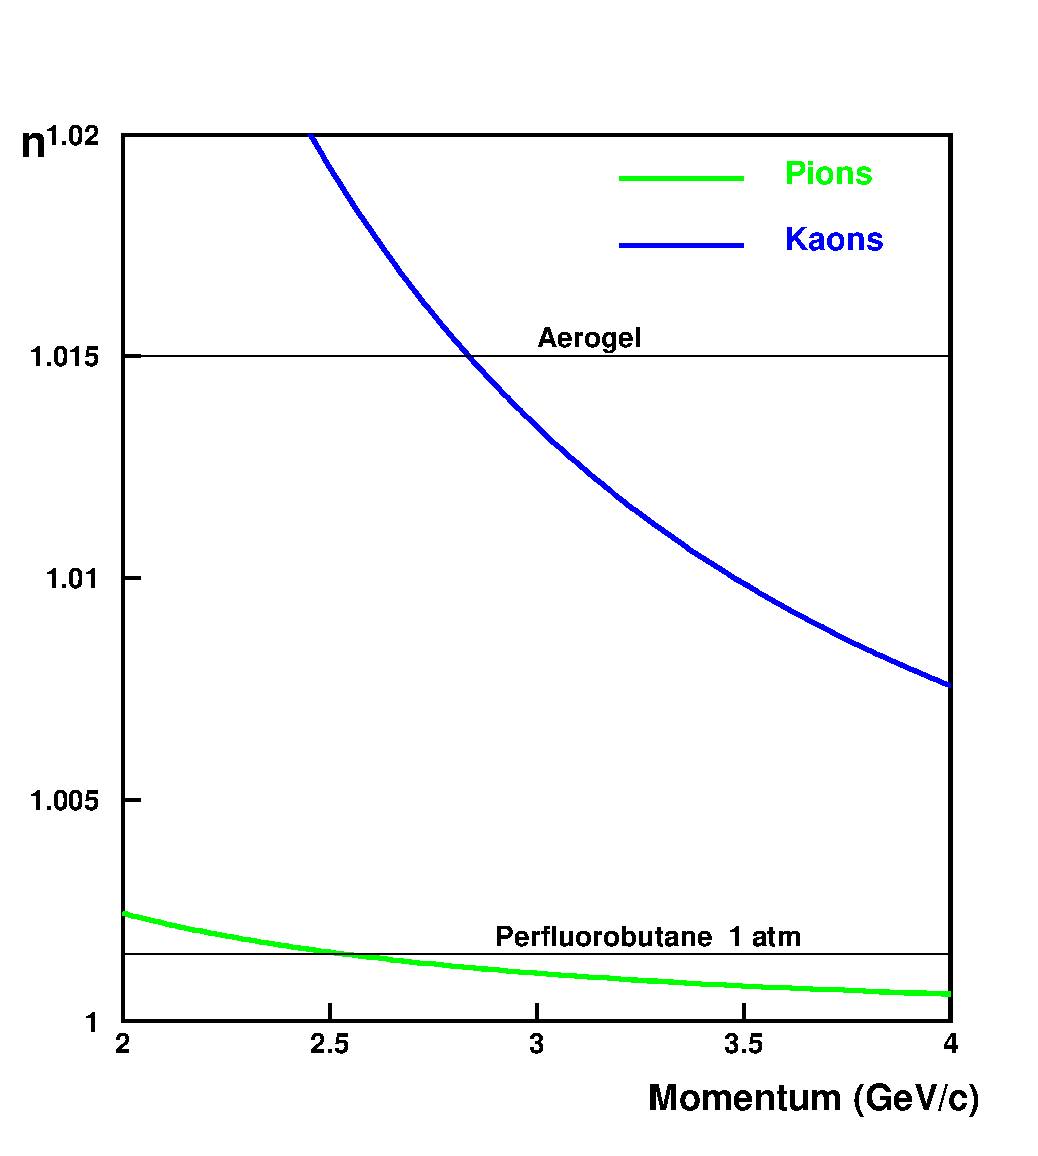
\includegraphics[width=0.8\columnwidth]{pid2}
  \caption[Gas $\breve{C}$erenkov detector.]{\label{fig:pid2}Gas $\breve{C}$erenkov detector.\\\\ Kaon and pion thresholds for producing $\breve{C}$erenkov radiation in the gas $\breve{C}$erenkov detector are shown by BLUE and GREEN curves, respectively.}
\end{figure}
%\setlength{\figwidth}{0.8\linewidth}
%\Figure{pid2}{\figwidth}{Gas $\breve{C}$erenkov detector: Kaon and pion thresholds for producing $\breve{C}$erenkov radiation in the gas $\breve{C}$erenkov detector are shown by \textcolor{blue}{BLUE} and \textcolor{green}{GREEN} curves, respectively.}

\SubSection{$\breve{C}$erenkov Radiation}%
%\label{$\breve{C}$erenkov}%
%Two type of $\breve{C}$erenkov i.e,. Aerogel and Gas $\breve{C}$erenkov have been used to identify particles in the experiment. The aerogel $\breve{C}$erenkov used in the experiment has a refractive index of n=1.015. In \figureref{pid1} the threshold for firing aerogel $\breve{C}$erenkov for proton, pion and kaon are shown in the \textcolor{red}{RED}, \textcolor{blue}{BLUE} and PURPPLE curve respectively. It is clear that protons never fire the aerogel and except for kinematics of $Q^2$ of 1.1 $GeV^2$ pion also do not fire, where as kaon always fire the aerogel. By applying a constraint over the aerogel we can seperate protons and pions from kaons. For the $Q^2$ of 1.1 $GeV^2$ kinematics, the aerogel can separete protons from pions and kaons. 
Two type of $\breve{C}$erenkov detectors, i.e, aerogel and gas $\breve{C}$erenkov, have been used to identify particles in the experiment. The aerogel $\breve{C}$erenkov detector used in the experiment has a refractive index of n = 1.015. In \figureref{pid1} we show the threshold for producing $\breve{C}$erenkov radiation by proton (RED curve), pions (GREEN curve), and kaons (BLUE curve). From this figure, we see that in our experiment the protons never produce $\breve{C}$erenkov radiation in the aerogel detector because the proton momentum in the experiment ($P_p$ = 2.7 - 3.4 $(GeV/c)$) is always above the threshold, while the kaons produce $\breve{C}$erenkov radiation for all kinematics except the $Q^2$ = 1.1 $(GeV/c)^2$ kinematics where the kaon momentum is $P_K$ = 2.7 $(GeV/c)$ which is above threshold for the aerogel. The pions are always below threshold and produce $\breve{C}$erenkov radiation for all kinematics. By applying cuts on the number of photo-electrons detected in the aerogel detector we could separate the protons from kaons and pions at all kinematics except $Q^2$ = 1.1 $(GeV/c)^2$. 

The gas $\breve{C}$erenkov detector uses perflurobutane at 1 atmosphere which has a refractive index of 1.0015. In \figureref{pid1}, the thresholds for pion and kaon are being shown by GREEN and BLUE curve, respectively. Kaons could be separated from pions by cutting on gas $\breve{C}$erenkov signal. If we apply cuts on the gas $\breve{C}$erenkov signal, then we will be able to separate kaons from pions. So, applying cuts on the two $\breve{C}$erenkov detectors we could separate kaons from pions and protons.

\Section{Cuts}
\label{Cuts}
The cuts applied on the reconstructed variables are shown in \tableref{cuts}. The cuts applied on data and the SIMC yields were the same for all cases. We have applied very tight cuts on all the variables to restrict the data to regions where the shape of that variable matches with SIMC yields.

\begin{table}
  \caption[Cuts applied on the reconstructed variables for data or SIMC.]{\label{tab:cuts}Cuts applied on the reconstructed variables for data or SIMC.}
\begin{center}
\begin{tabular}{||c|c|c||}\hline
 Variables & Left & Right \\
 & & \\\hline
Coincidence Time & -59.21 & -58.13 \\
$Missing Mass_\Lambda$ & 1.10 & 1.15 \\
$Missing Mass_\Sigma$ & 1.175 & 1.215 \\\hline
hsxptar & -0.075 & 0.075 \\
hsyptar & -0.03 & 0.03 \\
hsdelta & -10 & 5 \\
ssxptar & -0.065 & 0.065 \\
ssyptar & -0.0375 & 0.0375 \\
ssdelta & -18 & 5 \\\hline
$Q^2$ & 1.4 & 2.5 \\
W & 2.18 & 2.48 \\
t & 0.23 & 0.52 \\
$\phi_{pq}$ & 1.5 & 5 \\\hline
\end{tabular}
\end{center}
\end{table}
%\Table{cuts}{Cuts applied on the reconstructed variables for data or SIMC yields for kinematics of $Q^2$= 2.2 $(\mathrm{GeV/c})^2$.}

The cuts applied on data or SIMC yields for kinematics of $Q^2$= 2.2 $(\mathrm{GeV/c})^2$ have been shown in \tableref{cuts}. Most of the cuts applied on all the variables were quite similar for all the kinematics. We separated $\Lambda$ and $\Sigma$ production of $K^+$ for hydrogen data for all the variables. As we went to the heavier targets, the regions for $\Lambda$ and $\Sigma$ production seems to merge for almost all the variables and hence we were not able to separate them. So, the cuts applied for all other targets were similar with each other except for hydrogen.

\SubSection{Other Cuts}%
%
\label{Other Cuts}
Cuts were applied on several other reconstructed variables, such as \textit{hsxptar}, \textit{hsyptar}, \textit{ssxptar}, \textit{ssyptar}, \textit{hsdelta}, \textit{ssdelta}, etc., which define the feducial acceptance of the detector. These cuts have been applied to restrict the data to regions where they match the simulation. These cuts were discussed in the previous chapter.

%We have used several other PIDs like: hsxptar, hsyptar, ssxptar, ssyptar, hsdelta, ssdelta, hsbeta etc. Giving cuts over these PIDs we able to seperate different hadrons as well as reduce the background. As we had a very low stastictics, for thses other PIDs I applied very tight cut. The information that were avilable in the SIMC, I considered only that region. Means giving a very tight cut cosidered the common region for data and SIMC.

\Section{Comparison of Data with SIMC Yields}%
%
\label{Comparison of Data with SIMC Yields}
The cross section depends upon four variables; they are $Q^2$, $W$, $t$, $\phi_{pq}$, where $Q^2$ is four- momentum transferred square, $W$ is the C.M. energy, $t$ is momentum transfer, and $\phi_{pq}$ is  the angle between the scattering and reaction planes. So before calculating transparency, we compare the data with SIMC yields for these variables. If the simulated shape of these variables agree with the data, we can claim that the model used in the SIMC simulation is valid. After adding $\Lambda$ and $\Sigma$ production for $K^+$ with proper ratio obtained using hydrogen data, the yields are shown in \figureref{com_plot_2_Q2_2} for variable $Q^2$. The same procedure was applied to other variables as well. Comparison of data yields and SIMC yields for the variables $W$, $t$ and $\phi_{pq}$ after adding $\Lambda$ and $\Sigma$ production for $K^+$ are shown in \figureref{com_plot_2_w_2}, \figureref{com_plot_2_t_2} and  \figureref{com_plot_2_phi_2}, respectively.

\begin{figure}[!tbp]
  \centering
  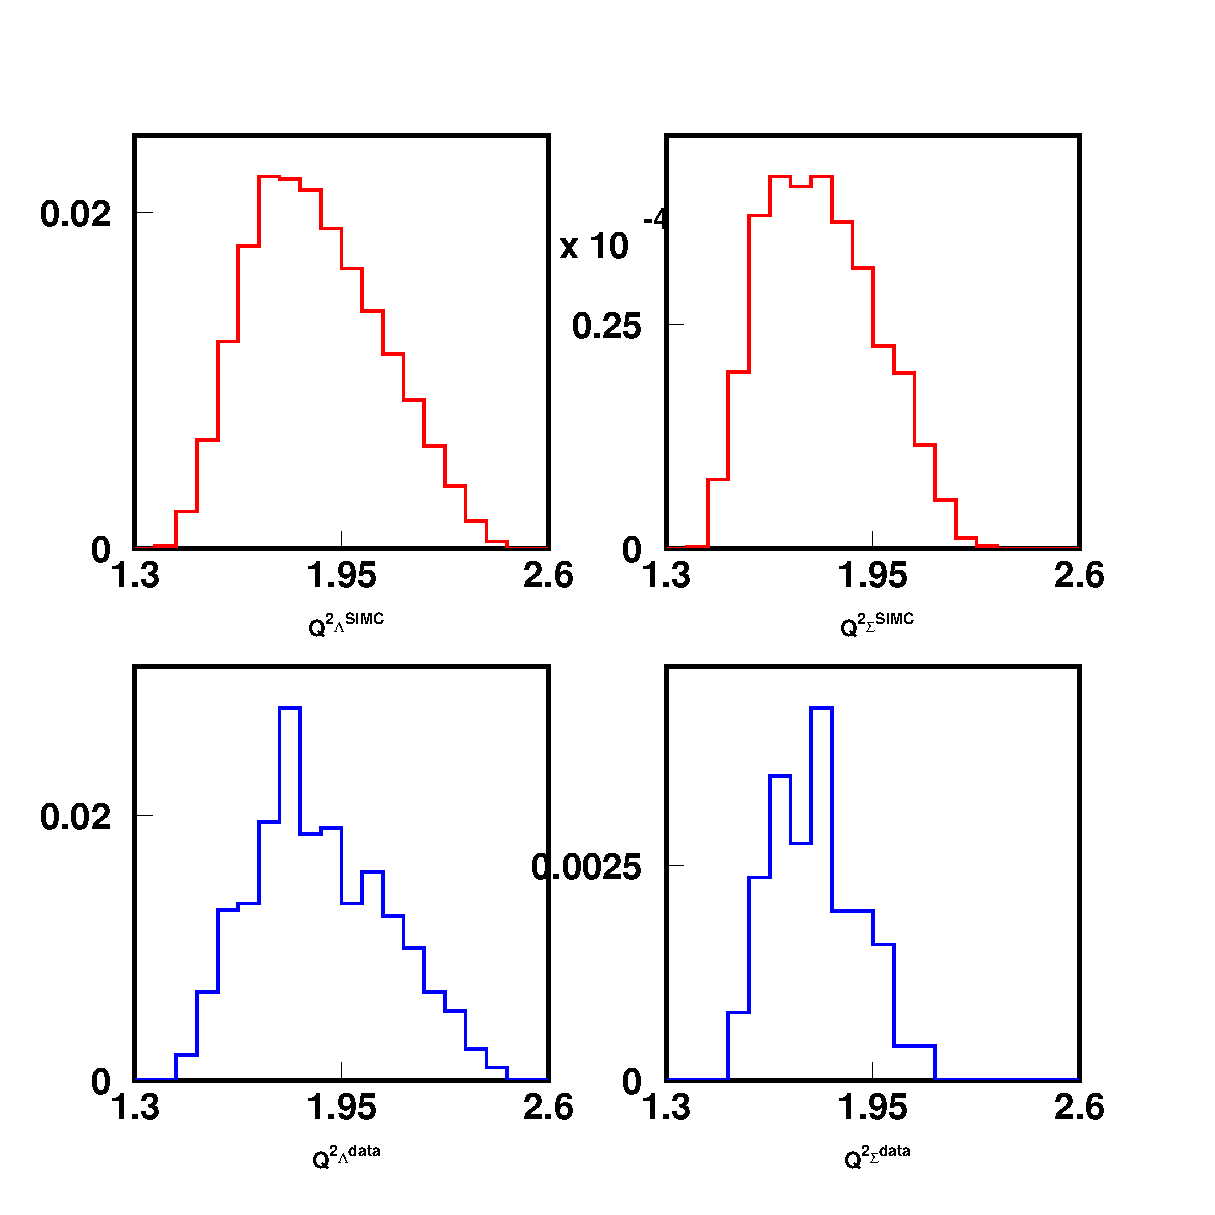
\includegraphics[width=0.8\columnwidth]{Q2_1}
  \caption[Comparison of $Q^2$ from data and SIMC.]{\label{fig:Q2_1}Comparison of $Q^2$ from data and SIMC.\\\\ Clockwise from top left corner: $Q^2_\Lambda$ SIMC, $Q^2_\Sigma$ SIMC, $Q^2_\Sigma$ data, $Q^2_\Lambda$ data for $Q^2$=2.2 $(\mathrm{GeV/c})^2$, where SIMC and data are shown in RED and BLUE, respectively.}
\end{figure}
%\setlength{\figwidth}{0.8\linewidth}
%\Figure{Q2_1}{\figwidth}{$Q^2$. Clockwise from top left corner: $Q^2_\Lambda$ SIMC, $Q^2_\Sigma$ SIMC, $Q^2_\Sigma$ data, $Q^2_\Lambda$ data for $Q^2$=2.2 $(\mathrm{GeV/c})^2$, where SIMC and data are shown in \textcolor{red}{RED} and \textcolor{blue}{BLUE}, respectively.}

%\setlength{\figwidth}{0.8\linewidth}
%\Figure{Q2_2}{\figwidth}{$Q^2$ combined $\Lambda$ and $\Sigma$ for both SIMC and data in \textcolor{red}{RED} and \textcolor{blue}{BLUE} respectively for $Q^2$=2.2 $GeV^2$}
\begin{figure}[!tbp]
  \centering
  \includegraphics[width=0.8\columnwidth]{com_plot_2_Q2_2}
  \caption[Comparison of $Q^2$ from data and SIMC.]{\label{fig:com_plot_2_Q2_2}Comparison of $Q^2$ from data and SIMC.\\\\ $Q^2$ combined $\Lambda$ and $\Sigma$ for both SIMC and data yields in RED and BLUE respectively for $(\mathrm{GeV/c})^2$.}
\end{figure}
%\setlength{\figwidth}{0.8\linewidth}
%\Figure{com_plot_2_Q2_2}{\figwidth}{$Q^2$ combined $\Lambda$ and $\Sigma$ for both SIMC and data yields in \textcolor{red}{RED} and \textcolor{blue}{BLUE} respectively for $(\mathrm{GeV/c})^2$.}

%\setlength{\figwidth}{0.8\linewidth}
%\Figure{w_1}{\figwidth}{W. Clockwise from top left corener: $W_\Lambda$ SIMC, $W_\Sigma$ SIMC, $W_\Sigma$ data, $W_\Lambda$ data for $Q^2$=2.2 $GeV^2$}
\begin{figure}[!tbp]
  \centering
  \includegraphics[width=0.8\columnwidth]{com_plot_2_w_2}
  \caption[Comparison of $W$ from data and SIMC.]{\label{fig:com_plot_2_w_2}Comparison of $W$ from data and SIMC.\\\\ $W$ combined $\Lambda$ and $\Sigma$ for both SIMC and data yields in RED and BLUE, respectively, for $Q^2$=2.2 $(\mathrm{GeV/c})^2$.}
\end{figure}
%\setlength{\figwidth}{0.8\linewidth}
%\Figure{com_plot_2_w_2}{\figwidth}{$W$ combined $\Lambda$ and $\Sigma$ for both SIMC and data yields in \textcolor{red}{RED} and \textcolor{blue}{BLUE}, respectively, for $Q^2$=2.2 $(\mathrm{GeV/c})^2$.}

%\setlength{\figwidth}{0.8\linewidth}
%\Figure{t_1}{\figwidth}{t. Clockwise from top left corener: $t_\Lambda$ SIMC, $t_\Sigma$ SIMC, $t_\Sigma$ data, $t_\Lambda$ data for $Q^2$=2.2 $GeV^2$}
\begin{figure}[!tbp]
  \centering
  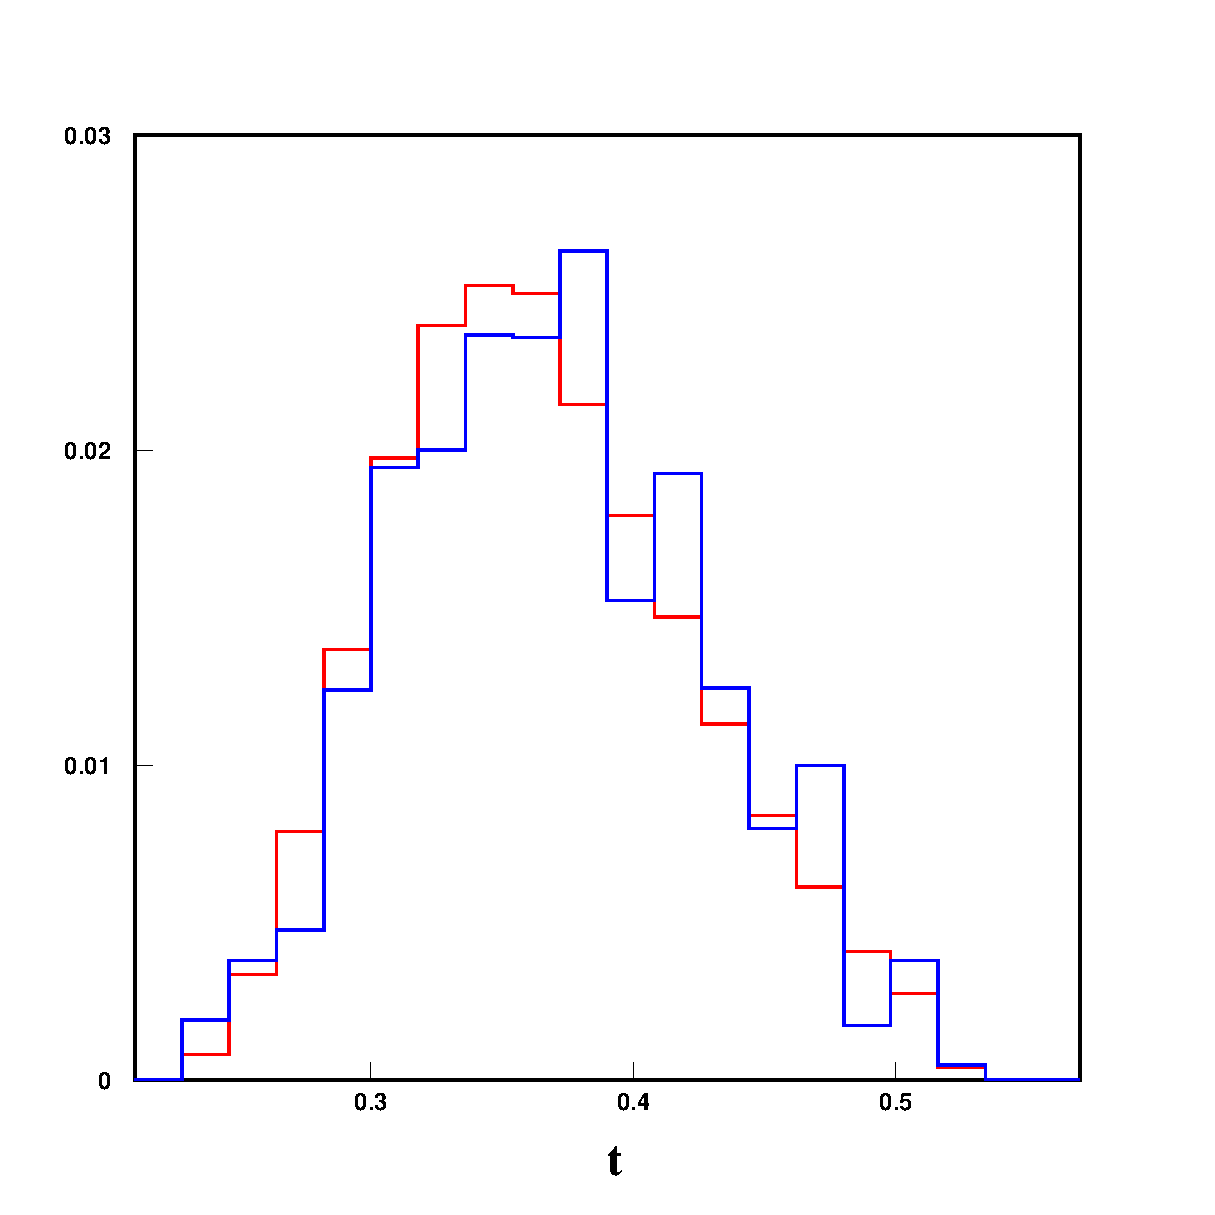
\includegraphics[width=0.8\columnwidth]{com_plot_2_t_2}
  \caption[Comparison of $t$ from data and SIMC.]{\label{fig:com_plot_2_t_2}Comparison of $t$ from data and SIMC.\\\\ $t$ combined $\Lambda$ and $\Sigma$ for both SIMC and data yields in RED and BLUE, respectively, for $Q^2$=2.2 $(\mathrm{GeV/c})^2$.}
\end{figure}
%\setlength{\figwidth}{0.8\linewidth}
%\Figure{com_plot_2_t_2}{\figwidth}{$t$ combined $\Lambda$ and $\Sigma$ for both SIMC and data yields in \textcolor{red}{RED} and \textcolor{blue}{BLUE}, respectively, for $Q^2$=2.2 $(\mathrm{GeV/c})^2$.}

%\setlength{\figwidth}{0.8\linewidth}
%\Figure{phipq_1}{\figwidth}{$\phi^{pq}$. Clockwise from top left corener: $\phi^{pq}_\Lambda$ SIMC, $\phi^{pq}_\Sigma$ SIMC, $\phi^{pq}_\Sigma$ data, $\phi^{pq}_\Lambda$ data for $Q^2$=2.2 $GeV^2$}
\begin{figure}[!tbp]
  \centering
  \includegraphics[width=0.8\columnwidth]{com_plot_2_phi_2}
  \caption[Comparison of $\phi_{pq}$ from data and SIMC.]{\label{fig:com_plot_2_phi_2}Comparison of $\phi_{pq}$ from data and SIMC.\\\\ $\phi_{pq}$ combined $\Lambda$ and $\Sigma$ for both SIMC and data yields in RED and BLUE, respectively, for $Q^2$=2.2 $(\mathrm{GeV/c})^2$.}
\end{figure}
%\setlength{\figwidth}{0.8\linewidth}
%\Figure{com_plot_2_phi_2}{\figwidth}{$\phi_{pq}$ combined $\Lambda$ and $\Sigma$ for both SIMC and data yields in \textcolor{red}{RED} and \textcolor{blue}{BLUE}, respectively, for $Q^2$=2.2 $(\mathrm{GeV/c})^2$.}

\chapter{Results}
%chapresult.tex
%
In this chapter, we will discuss the first measurement of the nucleon number $A$ and $Q^2$ dependence of nuclear transparency for the $A(e,e'K^+)$ process. Nuclear transparencies for $^{12}$C, $^{63}$Cu and $^{197}$Au nuclei over a  $Q^2$ range of 1.1 $\mathrm{to}$ 3.0 $(\mathrm{GeV/c})^2$ are shown with the super ratio of A$>$2 nuclei to deuterium.\footnote{Transparencies for these kinematic settings with the super ratio of A$>$1 nuclei to hydrogen are shown in APPENDIX \ref{Transparency with respect to Hydrogen}.} We also extracted average effective cross section for kaons in this kinematic range. We have compared our results with the available data to date.

%\Section{Cross sections}%
%Cross sections of Hydrogen target for three kinematics has been shown in \Tableref{t_1} and for all other targets have shown in \Tableref{t_2}.

\Section{Transparency}%
%
\label{Transparency}
The ratio of cross sections for exclusive processes from nuclei to those from nucleons is termed as Nuclear Transparency (T). The nuclear transparency was determined using the experimental charge-normalized yield, $\bar{Y}$ divided by the charge-normalized Monte Carlo equivalent yield, $\bar{Y}_{SIMC}$. For a given
target with nucleon number, A the nuclear transparency can be expressed as
\vspace{0.5in}
\begin{equation} \label{equ:nucltransp2}
T = 
\frac{\left(\bar Y/ \bar Y_{\rm MC} \right)_A}
{\left(\bar Y/ \bar Y_{\rm MC} \right)_{\rm D}},
\end{equation}

\noindent
where the denominator is the ratio of the yields for the deuterium target.
%\begin{center}$$T=\frac{\frac{\sigma_A^{Data}}{\sigma_A^{simc}}}{\frac{\sigma_0^{Data}}{\sigma_0^{simc}}}$$\end{center}

%\SubSection{Transparency with respect to Hydrogen}%
%\label{Transparency with respect to Hydrogen}
%Transparency of Kaon with respect to free nucleon cross section for three kinematics for all the targets has been shown in \Tableref{t_2}. We used Hydrogen cross section as free nucleon cross section. The total uncertinity has been taken as the qudrature sum of the statistical and systematic uncertinity. The differnt targets are shown by different colors as: black- $LD_2$, red- Carbon, green- Copper and blue- Gold for three different kinematics of $Q^2$= 1.1, 2.2 and 3.0 $(GeV/c)^2$. In the \figureref{transp1} the inner bar shows the statistical uncertinity and outer bar shows the systemetic uncertinity and total uncertinity as qudrature sum these two.


\SubSection{Transparency with Respect to Deuterium}%
Hydrogen consists of just one proton, and hence we considered its cross section as a free-nucleon cross section. But for all A$>$1 targets, we have neutrons. As deuterium has one proton and one neutron and one can produce ($K^+\Sigma^-$) from the neutron, therefore it is more appropriate to calculate transparency with respect to deuterium.\footnote{The transparencies with respect to the free-space cross section are shown in APPENDIX \ref{Transparency with respect to Hydrogen}.} Transparency of kaon with respect to $LD_2$ for three kinematics for all the targets are presented in \Tableref{t_4}. In \figureref{transp2} the variation of transparency with $Q^2$ is shown. Different targets are shown by different colors: (RED- Carbon, GREEN- Copper and BLUE- Gold) for the three different kinematic settings of $Q^2$= 1.1, 2.2 and 3.0 $(\mathrm{GeV/c})^2$. In \figureref{transp2}, the inner bar shows the statistical uncertainty and the outer bar shows the systematic uncertainty and total uncertainty as quadrature sum of these two.

\begin{table}
  \caption[T and $\sigma_{eff}$ for different targets with respect to $LD_2$.]{\label{tab:t_4}T and $\sigma_{eff}$ for different targets with respect to $LD_2$.}
\begin{center}
\begin{tabular}{||c|c|c|c|c|c|c||}\hline
 Target & $Q^2$ & Transparency & Statistical & Systematic & Total \\
 & $(GeV/c)^2$ & & error($\%$)& error($\%$)&error($\%$) \\\hline
Carbon & 1.1 & 0.90 &10.64 &16.11 &19.31\\
Copper & 1.1 & 1.06 &08.27 &10.83 &13.63\\
Gold   & 1.1 & 0.91 &11.63 &12.84 &17.32\\\hline
Carbon & 2.2 & 0.62 &09.39 &12.68 &15.78\\
Copper & 2.2 & 0.74 &07.24 &07.62 &10.52\\
Gold   & 2.2 & 0.79 &10.39 &13.65 &17.16\\\hline
Carbon & 3.0 & 0.43 &10.40 &07.13 &12.61\\
Copper & 3.0 & 0.60 &10.46 &07.60 &12.93\\
Gold   & 3.0 & 0.63 &14.03 &12.92 &19.07\\\hline
\end{tabular}
\end{center}
\end{table}
%\Table{t_4}{Transparency and cross section for different targets and of $Q^2$ for kaon with respect to the cross section of $LD_2$.}
%\begin{singlespace}
% Different kinematic settings for kaon with respect to the cross section of $LD_2$ are shown here.
%\end{singlespace}

\begin{figure}[!tbp]
  \centering
  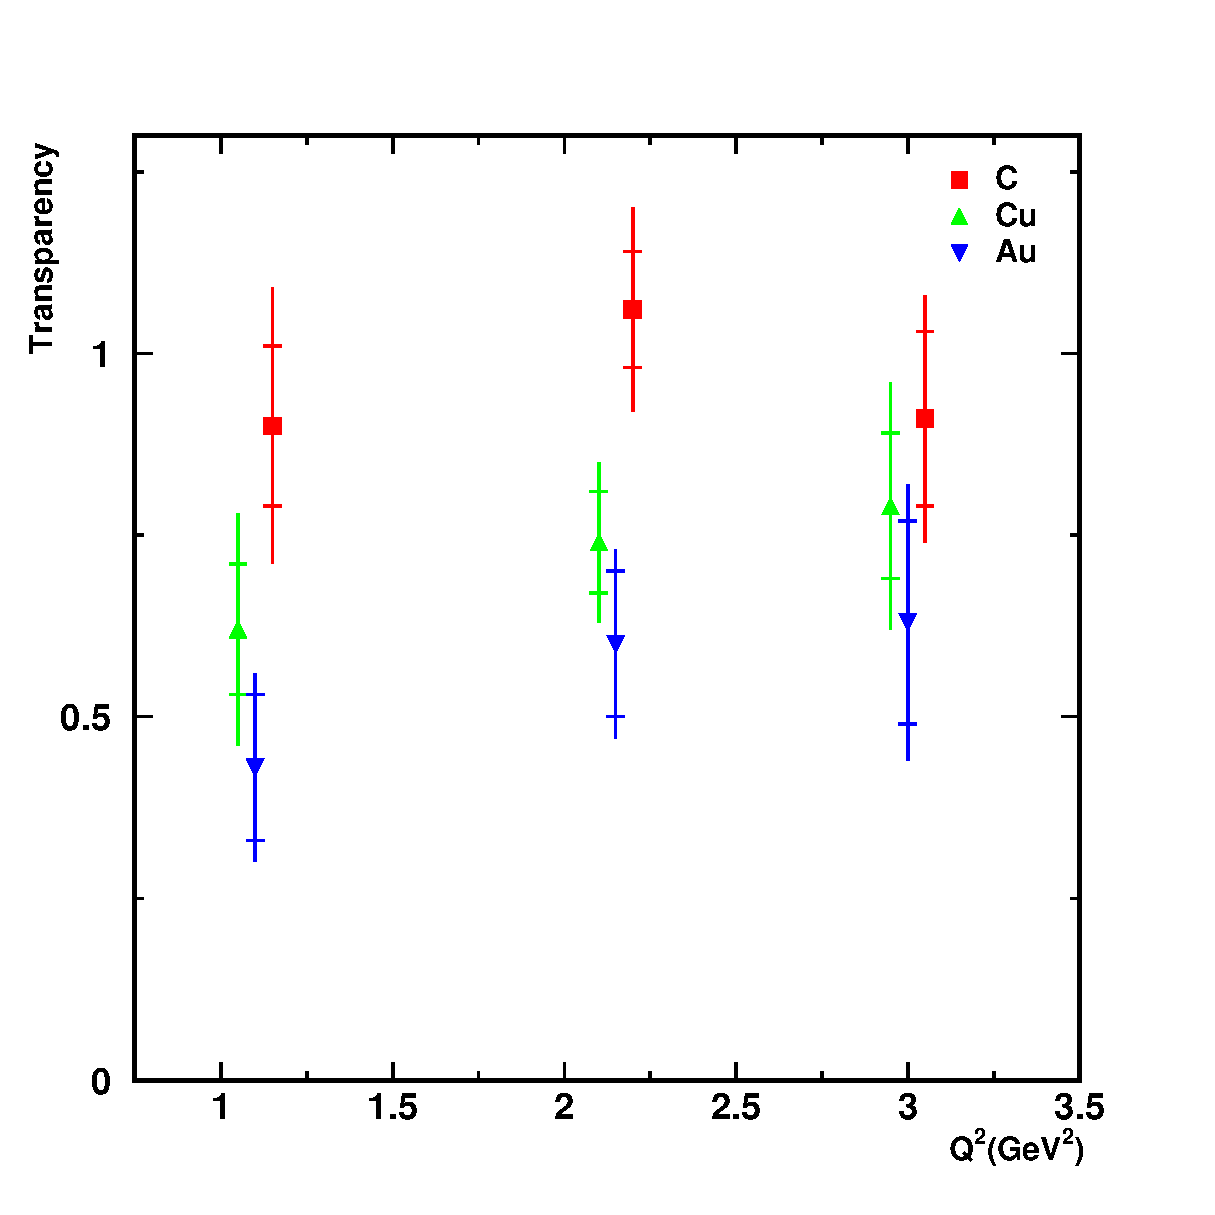
\includegraphics[width=0.8\columnwidth]{transp2}
  \caption[Nuclear transparency for targets of $A>$2 with respect to $LD_2$.]{\label{fig:transp2}Nuclear transparency for targets of $A>$2 with respect to $LD_2$.\\\\ Carbon and copper are shifted by 0.05 and -0.05 $(\mathrm{GeV/c})^2$ in $Q^2$, respectively, with respect to gold for convenience. The targets are shown in different colors as RED- carbon, GREEN- copper and BLUE- gold.}
\end{figure}
%\setlength{\figwidth}{0.8\linewidth}
%\Figure{transp2}{\figwidth}{Nuclear transparency for targets of $A>$2 with respect to $LD_2$. Carbon and copper are shifted by 0.05 and -0.05 $(\mathrm{GeV/c})^2$ in $Q^2$, respectively, with respect to gold for convenience. The targets are shown in different colors as \textcolor{red}{RED}- carbon, \textcolor{green}{GREEN}- copper and \textcolor{blue}{BLUE}- gold.}

%\Figure{alpha}{\figwidth}{$\alpha$ for differnt kinematics with theoritical band.}
%
\Section{Error Calculation}%
\label{Error Calculation}
In this section we briefly describe the error analysis for the statistical and systematic error in the experiment.

\SubSection{Statistical Error Calculation}%
\label{Statistical Error Calculation}
The statistical uncertainties in the charge-normalized experimental yields were calculated for each run and summed over the runs at a given kinematic setting. The total charge-normalized yield can be written as

\begin{equation} \label{equ:staterror1}
\bar{Y} = 
\left(\sum^{n}_{i}\frac{\bar{Y}_i}{(\bar{Y}_i/\sqrt{N_i})^2}\right)
\left(\sum^{n}_{i}\frac{1}{(\bar{Y}_i/\sqrt{N_i})^2}\right)^{-1}
\end{equation}

\noindent
where $i$ represents the $i^{th}$ run of a kinematic setting and $N_i$ is the number of events inside the experimental acceptance. The statistical uncertainty for the entire setting, $d\bar{Y}$ , can be written as

\begin{equation} \label{equ:staterror2}
d\bar{Y} = 
\left(\sum^{n}_{i}N_i/\bar{Y}_i^2\right)^{-\frac{1}{2}}
\end{equation}

We applied the same acceptance and missing mass cuts to both the experimental data and the Monte Carlo events. The Monte Carlo statistical error was determined in a similar fashion, except $N_i$ was replaced with the raw number of Monte Carlo particles that passed these cuts. Then statistical uncertainty in the transparency, $dT_{stat}$, was given by \cite{BC06}

\begin{equation} \label{equ:staterror3}
dT_{stat} = 
T \times \sqrt{\left(\left[d\bar{Y}/\bar{Y}\right]^2 + \left[d\bar{Y}_{SIMC}/\bar{Y}_{SIMC}\right]^2 \right)_A + 
\left(\left[d\bar{Y}/\bar{Y}\right]^2 + \left[d\bar{Y}_{SIMC}/\bar{Y}_{SIMC}\right]^2\right)_D}
\end{equation}

\SubSection{Systematic Error Calculation}%
\label{Systematic Error Calculation}
%We used same systemetic uncertinities from pion transparecy calculation \cite{BC06} except the uncertinities Particle ID and Cut Dependence. 
As we are using the same set of data from experiment E01-107 as used in pion transparency analysis, most of the uncertainties are same as determined during the  pion transparency analysis \cite{BC06}. The two uncertainties that differ are uncertainty in particle identification and cut dependence. An important aspect was to investigate the stability of the results as a function of the applied cuts. The cut dependence was calculated by measuring the variation of yield due to systematic variation of the cuts. 
The standard deviation of the resulting yields was used as an estimate of the systematic uncertainty on the quoted yield. For different targets and different kinematic settings, uncertainties were different. List of systematic uncertainties is shown in \Tableref{err_1}.

\begin{table}
  \caption[Systematic Error.]{\label{tab:err_1}Systematic Error.}
\begin{center}
\begin{tabular}{||c|c|c|c||}\hline
 Item & Point to Point($\%$) & Scale($\%$) & Total($\%$) \\\hline
Particle ID 				 & 2.0 & 0.4- 0.7 & \\\hline
Charge 							 & 0.3 & 		0.5	  & \\
Target Thickness 		 & 0.5 & 			    & \\
Coin Blocking 			 & 0.1 & 				  & \\
Trigger(HMS+SOS)  	 & 0.7 & 				  & \\
Dead Time Correction & 0.1 & 				  & \\
Tracking(HMS+SOS) 	 & 0.5 & 		0.5	  & \\
Kaon Abosorption	 	 & 0.5 &    2.0	  & \\
Beam Energy					 & 0.1 &    0.1   & \\\hline
Cut Dependence		 	 & 2.5 & 		0.5	  & \\\hline
Kaon Decay				 	 & 0.5 & 		1.0	  & \\
Pauli Blocking		 	 & 0.5 & 				  & \\
Radiative Correction & 0.5 & 		1.0	  & \\
Collimator				 	 & 1.0 & 				  & \\
Acceptance				 	 & 0.5 &		2.0		& \\
Spectral Function		 & 1.0 & 		2.0	  & \\\hline\hline
Total							 	 & 3.8 & 		3.9	  & 5.4\\\hline
\end{tabular}
\end{center}
\end{table}
%\Table{err_1}{Systematic Error.}

%
\Section{Effective Cross Section}%
%
We can analyze the transparency results from the different nuclei and the different experiments in
terms of a simple geometric model \cite{ON95, jain}. This model assumes classical attenuation of protons propagating in the nucleus, with an effective nucleon-nucleon cross section $\sigma_{eff}$ that is independent of density.

The effective cross section has a relation with transparency as

\begin{equation} \label{equ:eff1}
T_{hadron} = {\frac{1}{Z}}\int d^{3}r \rho_{z}(\vec{r})exp\left[-\int dz'\sigma_{eff} \rho_{A-1}(\vec{r}^\prime)\right]
\end{equation}

\noindent
where $\rho_z(\vec{r})$ is charge density distribution along z at $\vec{r}$ and  $\rho_{A-1}(\vec{r^\prime})$ is at $\vec{r^\prime}$ for the ($A$-1) nucleon. $Z$ is the number of protons. $\sigma_{eff}$ is independent of density and only a free parameter in the equation.

\begin{table}
  \caption[Effective cross section for different targets and of $Q^2$ for kaons.]{\label{tab:eff_cr1}Effective cross section for different targets and of $Q^2$ for kaons.}
\include{eff_cr1}
\end{table}
%\Table{eff_cr1}{Effective cross section for different targets and of $Q^2$ for kaons}

\SubSection{Effective Cross Section of Kaons($K^+$)}%
\label{Effective cross-section of kaons($K^+$)}
Kaon-nucleon effective cross section vs transparency for different targets have been plotted in \figureref{eff_t_all}. We have extracted the effective cross section corresponding to the measured transparencies using these dependencies of transparency and effective cross section. For example, the measured transparency at $Q^2$ = 1.1 $(\mathrm{GeV/c})^2$ is shown by vertical lines in \figureref{eff_t_all} and the corresponding effective cross section is shown by horizontal lines. Similarly we have calculated effective kaon-nucleon cross section for all kinematic settings which are given in \Tableref{eff_cr1}.

\begin{figure}[!tbp]
  \centering
  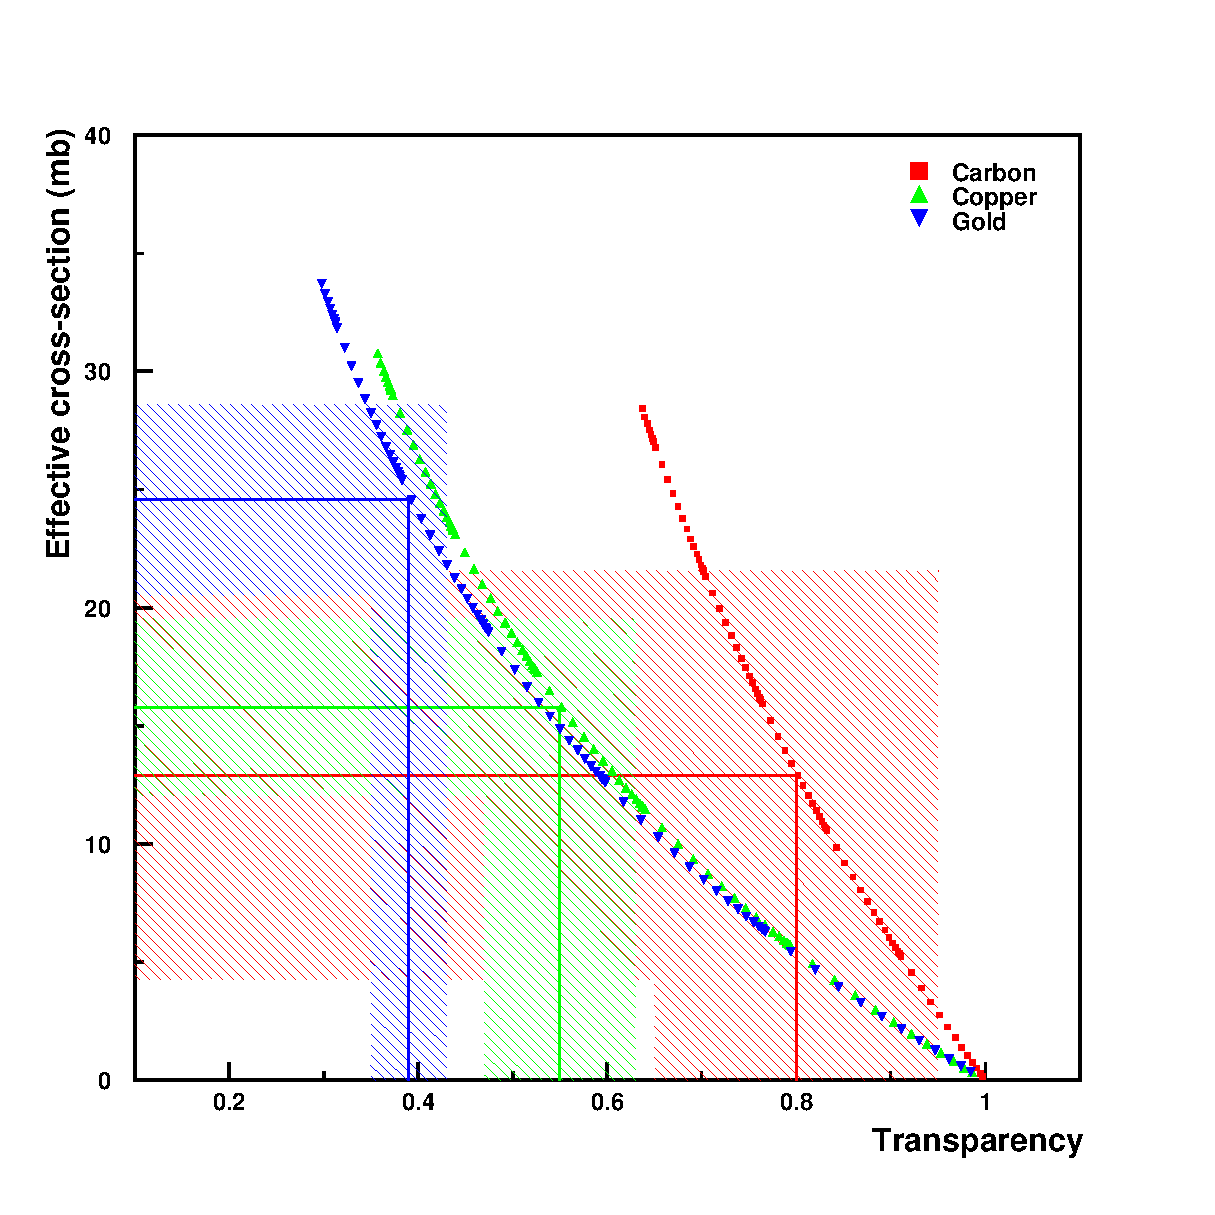
\includegraphics[width=0.8\columnwidth]{eff_t_all}
  \caption[Effective cross section comparison.]{\label{fig:eff_t_all}Effective cross section comparison.\\\\ Data points in RED are for carbon, GREEN data points are for copper and BLUE data points are for gold, considering only statistical uncertainty for kinematics1($Q^2$=1.1 $(\mathrm{GeV/c})^2$).}
\end{figure}
%\setlength{\figwidth}{0.8\linewidth}
%\Figure{eff_t_all}{\figwidth}{Effective cross section comparison. Data points in \textcolor{red}{RED} are for carbon, \textcolor{green}{GREEN} data points are for copper and \textcolor{blue}{BLUE} data points are for gold, considering only statistical uncertainty for kinematics1($Q^2$=1.1 $(\mathrm{GeV/c})^2$).}

The average effective cross section has been calculated for different kinematic settings by weighted average over different targets, as shown in Eq. \ref{equ:effective}. The average effective cross sections for $K^+$ are listed in \Tableref{eff_cr2} and shown in \figureref{eff_av_all} in BLUE.

\begin{equation} \label{equ:effective}
\sigma_{eff}^{av} = 
\frac{\left(1/\sigma_{err}^{C}\right)^{2}\sigma_{eff}^{C}+ \left(1/\sigma_{err}^{Cu}\right)^2\sigma_{eff}^{Cu}+
\left(1/\sigma_{err}^{Au}\right)^2\sigma_{eff}^{Au}}
{\left(1/\sigma_{err}^{C}\right)^2+ \left(1/\sigma_{err}^{Cu}\right)^2+\left(1/\sigma_{err}^{Au}\right)^2}
\end{equation}

\Table{eff_cr2}{Average effective cross section for different $Q^2$ for kaons.}

\begin{table}
  \caption[Effective cross section for different targets and of $Q^2$ for pion.]{\label{tab:eff_cr3}Effective cross section for different targets and of $Q^2$ for pion.}
\begin{center}
\begin{tabular}{||c|c|c|c|c||}\hline
 Target & $Q^2$ & $P_k$ & Transparency & Effective cross section \\
 & $(GeV/c)^2$ & $(GeV/c)$ & & (mb)\\\hline
Carbon & 1.1 & 2.8 & 0.67$\pm$0.01 &24.82$\pm$1.12 \\
Copper & 1.1 & 2.8 & 0.45$\pm$0.01 &22.34$\pm$0.75 \\
Gold   & 1.1 & 2.8 & 0.28$\pm$0.01 &35.99$\pm$1.38 \\\hline
Carbon & 2.2 & 3.2 & 0.65$\pm$0.01 &27.07$\pm$1.32 \\
Copper & 2.2 & 3.2 & 0.45$\pm$0.01 &22.34$\pm$0.75 \\
Gold   & 2.2 & 3.2 & 0.29$\pm$0.01 &34.73$\pm$1.34 \\\hline
Carbon & 3.0 & 3.4 & 0.68$\pm$0.02 &23.77$\pm$2.20 \\
Copper & 3.0 & 3.4 & 0.43$\pm$0.01 &23.83$\pm$0.66 \\
Gold   & 3.0 & 3.4 & 0.29$\pm$0.01 &34.73$\pm$1.34 \\\hline
Carbon & 3.9 & 4.1 & 0.77$\pm$0.02 &15.21$\pm$1.58 \\
Copper & 3.9 & 4.1 & 0.52$\pm$0.01 &17.56$\pm$0.48 \\
Gold   & 3.9 & 4.1 & 0.34$\pm$0.01 &28.84$\pm$0.98 \\\hline
Carbon & 4.7 & 4.4 & 0.70$\pm$0.03 &21.67$\pm$3.00 \\
Copper & 4.7 & 4.4 & 0.53$\pm$0.02 &17.20$\pm$1.21 \\
Gold   & 4.7 & 4.4 & 0.33$\pm$0.02 &30.23$\pm$1.38 \\\hline
\end{tabular}
\end{center}
\end{table}
%\Table{eff_cr3}{Effective cross section for different targets and of $Q^2$ for pion.}

\SubSection{Effective Cross Section of Pions ($\pi^+$)}%
%\label{Effective crorss-section of pions($\pi^+$)}
Applying the same technique used in section \ref{Effective cross-section of kaons($K^+$)}, we have calculated the effective $\pi^+$-nucleon cross section from the measured pion transparency \cite{BC06}. The effective cross sections for different targets for five kinematic settings of $Q^2$ = 1.1, 2.2, 3.0, 3.9 and 4.7 $(\mathrm{GeV/c})^2$ are shown in \Tableref{eff_cr3}. Average cross sections are listed in \Tableref{eff_cr4} and shown in \figureref{eff_av_all} in GREEN.

\Table{eff_cr4}{Average effective cross section for different $Q^2$ for pion.}

\begin{figure}[!tbp]
  \centering
  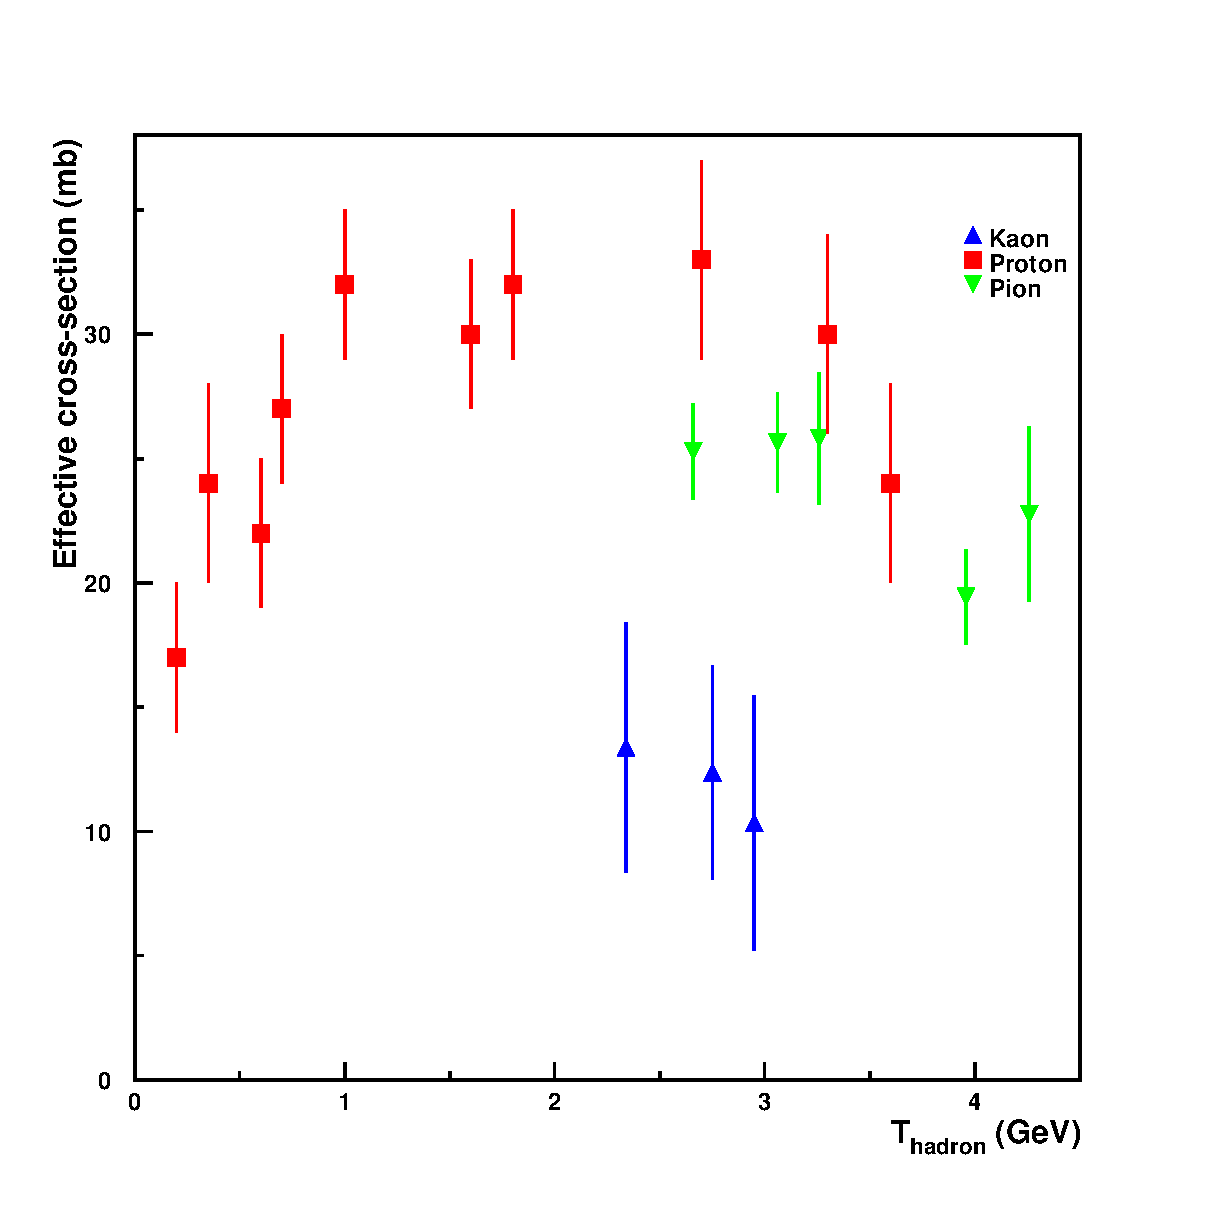
\includegraphics[width=0.8\columnwidth]{eff_av_all}
  \caption[Effective cross section vs transparency.]{\label{fig:eff_av_all}Effective cross section vs transparency.\\\\ Data points in RED is for protons, GREEN data points are for $\pi^+$ and BLUE data points are from this analysis for $K^+$, considering only statistical uncertainty \cite{hinton01}.}
\end{figure}
%\setlength{\figwidth}{0.8\linewidth}
%\Figure{eff_av_all}{\figwidth}{Effective cross section vs transparency. Data points in \textcolor{red}{RED} is for protons, \textcolor{green}{GREEN} data points are for $\pi^+$ and \textcolor{blue}{BLUE} data points are from this analysis for $K^+$, considering only statistical uncertainty \cite{hinton01}.}

\SubSection{Effective Cross Section of Protons (p)}%
\label{Effective cross-section of protons(p)}
The average effective cross section for different kinematic settings for protons are listed in \Tableref{eff_cr6} from reference\cite{carroll} and shown in \figureref{eff_av_all} by RED.

\Table{eff_cr6}{Average effective cross section for different $T_K$ for protons\cite{jlabp2}.}

\SubSection{Effective Cross Section for All Hadrons ($\pi^+$, $K^+$, p)}%
The world data \cite{PDG} on p-p, p-n total cross sections as a function of kinetic energy ($T_{hadron}$) was fitted to a function form as shown in \figureref{crr1}. The error bars are statistical only. $T_{hadron}$ is defined as 

\begin{equation} \label{equ:effective4}
T_{hadron} = \sqrt{P_{hadron}^2 + M_{hadron}^2} - M_{hadron}
\end{equation}

We also performed similar fits for the world $\pi^+$-p, $\pi^+$-n and $K^+$-p, $K^+$-n data as shown in \figureref{crr1}. We then compared the effective cross section extracted from our experiment to these fitted forms for the proton, pion and kaon. The results are shown in \figureref{crr2} with RED for protons, GREEN for pions and BLUE for kaons. 

%where $P_{hadron}$ and $M_{hadron}$ are the momentum and mass of the hadron respectively. Using this formula we have calculated the kinetic energy for kaons, pions and protons corresponding to different kinematic settings. The world data for p-p, p-n and n-n elastic scattering data were fited to compare with data and has been shown in the \figureref{crr1}. The error bar represent the ststistical uncertinity. In the \figureref{crr2} we have ploted the effective proton-nucleon cross section from 
%\Tableref{eff_cr6} for different kinematic settings with world data fit \cite{PDG} in \textcolor{red}{RED}. Similarly for pions and kaons are shown in \textcolor{green}{GREEN} and \textcolor{blue}{BLUE} respectively.
\Table{scalefactor}{Scale factors for different hadron-nucleon scattering.}

Note that the world data of hadron-nucleon scattering cross sections are obtained from hadron scattering experiments. In this analysis, we compared the electron scattering effective cross section with those obtained from hadron-scattering experiments.

The scale factors in \Tableref{scalefactor} indicate the differences in the nature of the probes used: electromagnetic for electrons vs strong for hadrons. Since the electromagnetic interaction is weaker than the strong interaction, hence electrons can probe deeper into the nucleus compare to hadrons. This leads the scale factors between electron-scattering and hadron-scattering technique. The remarkable agreement between the K.E. dependence of the proton cross sections obtained from electron scattering and hadron scattering point to the similar reaction mechanisms that are well described within traditional nuclear physics. The deviation of the pion results indicate a break down of traditional nuclear physics reaction mechanisms for pions. For the kaons, our uncertainties are too large to draw any conclusions.

\begin{figure}[!tbp]
  \centering
  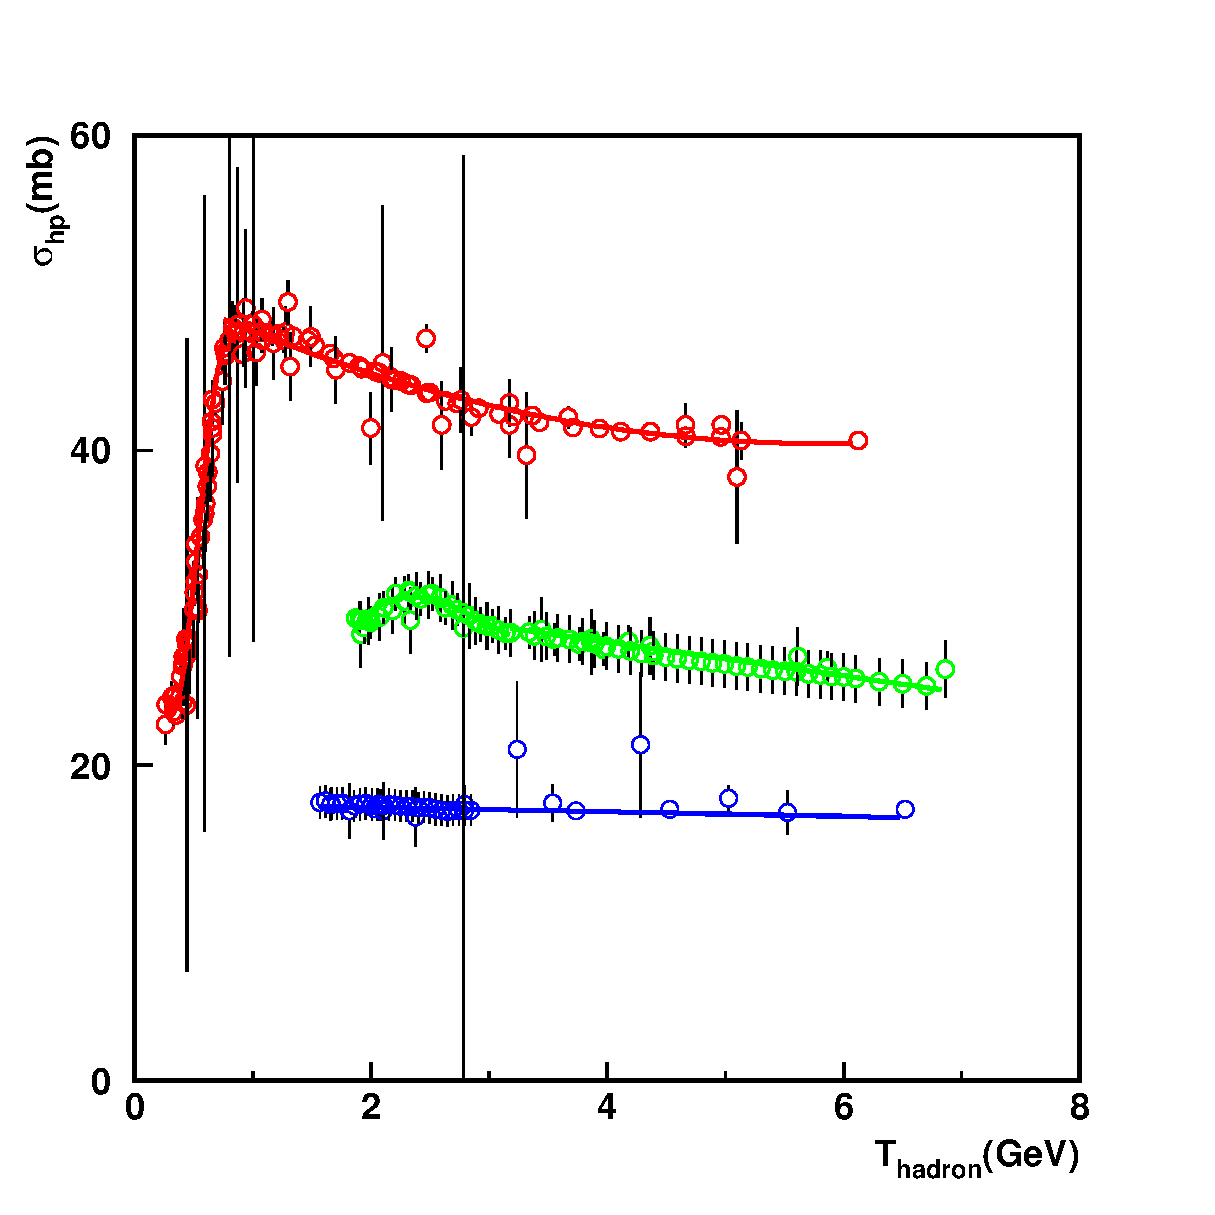
\includegraphics[width=0.8\columnwidth]{crr1}
  \caption[Hadron-proton total cross section vs $T_{hadron}$.]{\label{fig:crr1}Hadron-proton total cross section vs $T_{hadron}$.\\\\ Data points in RED are for protons, GREEN data points are for $\pi^+$ and BLUE data points are from this analysis for $K^+$ from \cite{hinton01}.}
\end{figure}
%\setlength{\figwidth}{0.8\linewidth}
%\Figure{crr1}{\figwidth}{Hadron-proton total cross section vs $T_{hadron}$: Data points in \textcolor{red}{RED} are for protons, \textcolor{green}{GREEN} data points are for $\pi^+$ and \textcolor{blue}{BLUE} data points are from this analysis for $K^+$ from \cite{hinton01}.} 

\begin{figure}[!tbp]
  \centering
  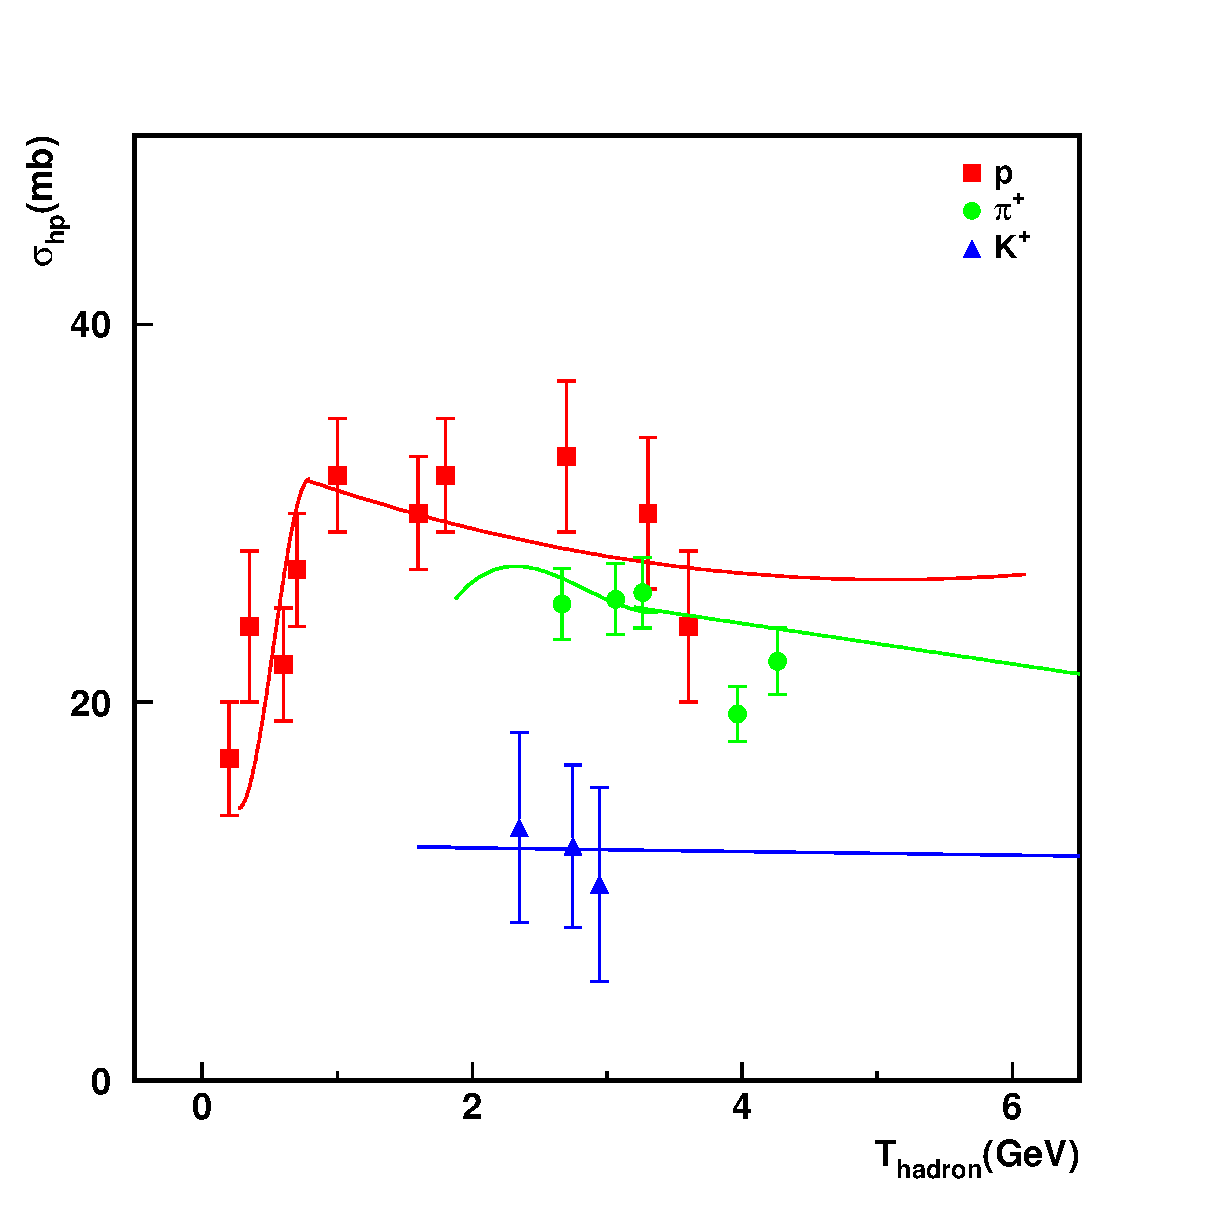
\includegraphics[width=0.8\columnwidth]{crr2}
  \caption[Comparison of effective and hadron-proton total cross section.]{\label{fig:crr2}Comparison of effective and hadron-proton total cross section.\\\\ Data points in RED are for protons from \cite{hinton01}, GREEN data points are for $\pi^+$ and BLUE data points are from this analysis for $K^+$. The fits are from hadron-scattering world data\cite{PDG} with scale factors given in \Tableref{scalefactor}.}
\end{figure}
%\setlength{\figwidth}{0.8\linewidth}
%\Figure{crr2}{\figwidth}{Effective cross section vs $T_{hadron}$: Data points in \textcolor{red}{RED} are for protons from \cite{hinton01}, \textcolor{green}{GREEN} data points are for $\pi^+$ and \textcolor{blue}{BLUE} data points are from this analysis for $K^+$. The fits are from hadron-scattering world data\cite{PDG} with scale factors given in \Tableref{scalefactor}.} 

\SubSection{$A$ Dependency of Transparency}%
The $A$ dependence of the nuclear transparency is extracted from the simple ansatz $T = A^{1 - \alpha}$, where $\alpha$ is used to parametrize the nuclear cross section and $\sigma_N$ is in terms of the elementary nucleon cross-section, $\sigma_{0}$ as $\sigma_N = \sigma_0A^{\alpha}$.

%From the observation what we found is kaon is mostly transparent.
\begin{table}
  \caption[$\alpha$ values for different $Q^2$ for kaons with respect to $LD_2$.]{\label{tab:alpha2}$\alpha$ values for different $Q^2$ for kaons with respect to $LD_2$.}
\begin{center}
%\centering
\begin{tabular}{||c|c|c||}\hline
 Kinematics & $Q^2$ & $\alpha$ \\
 & $(GeV/c)^2$ & \\\hline
Kin1 & 1.1 &0.84$\pm$0.06 \\
Kin2 & 2.2 &0.91$\pm$0.04 \\
Kin3 & 3.0 &0.92$\pm$0.05 \\\hline
\end{tabular}
\vspace{-0.5cm}
\end{center}
\end{table}
%\Table{alpha2}{$\alpha$ values for different $Q^2$ for kaons with respect to $LD_2$.}

The $Q^2$ dependence of nuclear transparency was very small for the kinematics range of $Q^2$= 1.1 $(\mathrm{GeV/c})^2$ to $Q^2$= 3.0 $(\mathrm{GeV/c})^2$. Fitting the transparency for a particular $Q^2$ to T = $A^{1-\alpha}$, we get $\alpha$ as shown in \Tableref{alpha2}.\footnote{The value of $\alpha$ with respect to hydrogen is given in APPENDIX A, \Tableref{alpha1}.} We extracted transparency and effective cross section for different kinematic settings for kaons in this analysis and calculated effective cross sections for available transparencies for protons and pions. $\alpha$ values have been plotted against effective cross section from this work and reference \cite{jlabp2} in \figureref{carolplot}.

\begin{figure}[!tbp]
  \centering
  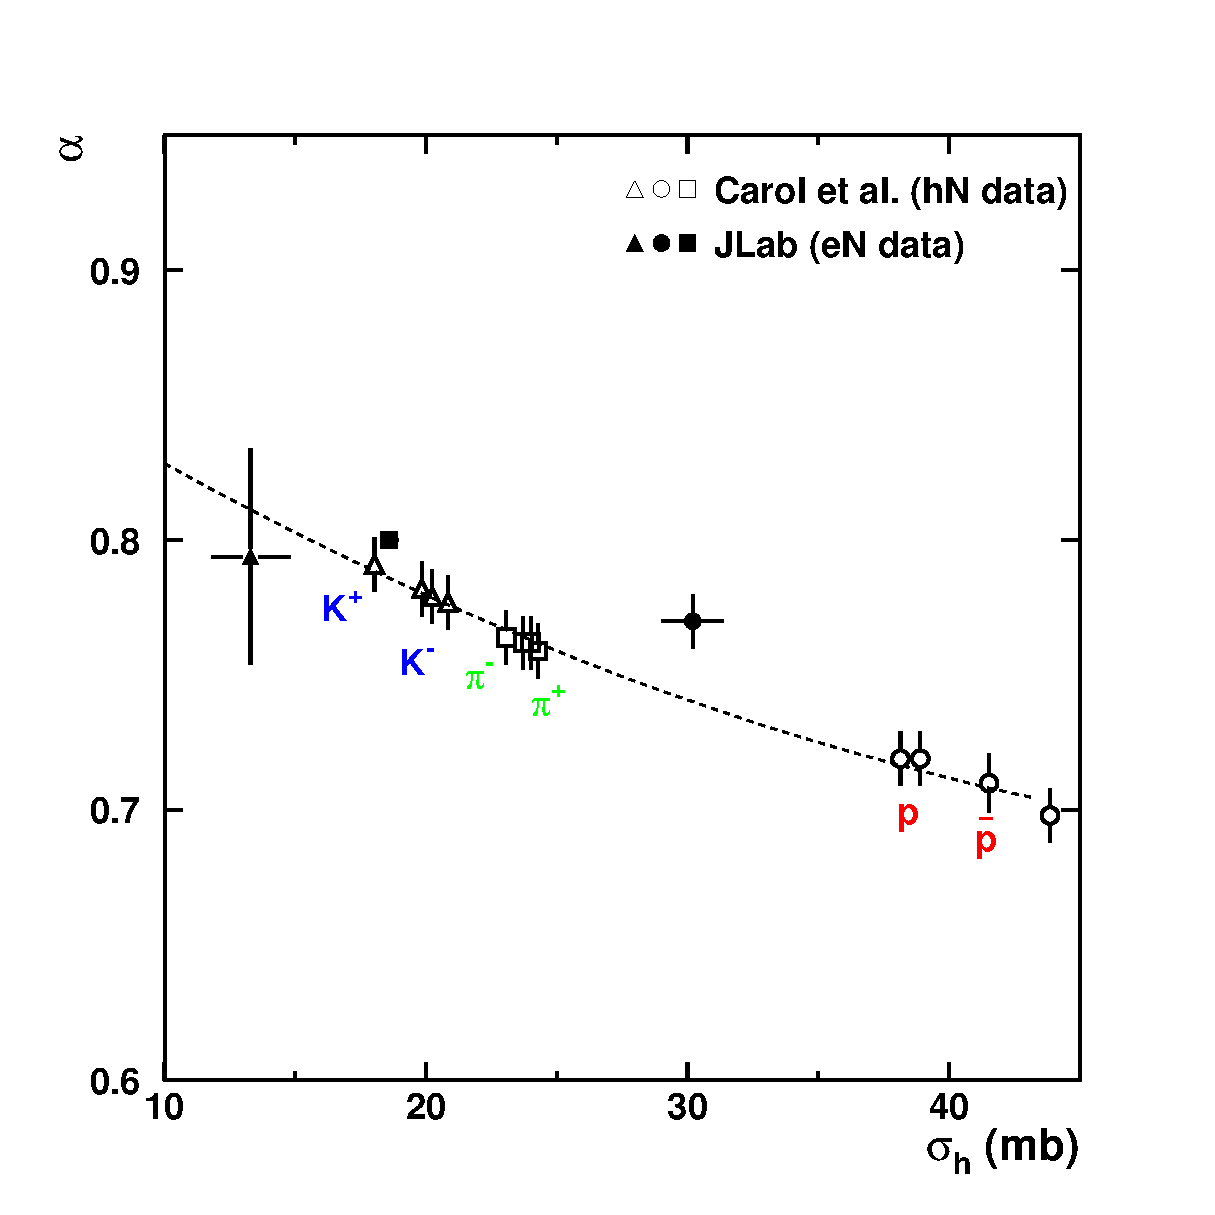
\includegraphics[width=0.8\columnwidth]{carolplot}
  \caption[$\alpha$ from electro-production of hadrons and from hadron-scattering.]{\label{fig:carolplot}$\alpha$ from electro-production of hadrons and from hadron-scattering.\\\\ $\alpha$ from electro-production of kaons (from this analysis), pions, and protons are shown by solid triangle, square, and cicrle, respectively. Similarly, $\alpha$ from hadron-scattering reactions are shown by empty points and fitted with dotted curve \cite{carroll}.}
\end{figure}
%\setlength{\figwidth}{0.8\linewidth}
%\Figure{carolplot}{\figwidth}{$\alpha$ from electro-production of kaons (from this analysis), pions, and protons are shown by solid triangle, square, and cicrle, respectively. Similarly, $\alpha$ from hadron-scattering reactions are shown by empty points and fitted with dotted curve \cite{carroll}.}

The results indicate that the effective cross section obtained from electron-scattering is smaller than hadron-scattering (as expected from the nature of the probe). For protons and pions, the parameter $\alpha$ extracted from electro-production measurements do not agree with those obtained from hadro-production, some of these differences may also be related to the strength of the interaction between the incident hadron and the nucleons. For kaons, the parameter $\alpha$ from electro-production is consistent within statistical uncertainties, with those obtained from hadro-production. However, due to the low statistics of kaons in our data set, we cannot draw any strong conclusions.
%The results indicate that not only the effective cross section obtained from electron-scattering is smaller than hadron-scattering (as expected from the nature of the probe). For protons and pions, $\alpha$ extracted from electro-production  measurements do not agree with those obtained from hadro-production but for kaons, the $\alpha$ are consistent within statistical uncertainties. Due to low statistics of kaons in our data set, our results do not draw any strong conclusions. 

\chapter{Conclusions}
%chapdiscussion.tex
%
\Section{Conclusions}
\label{Conclusion}
The nuclear transparency of kaons in the reaction $A(e,e'K^+)$ was measured by forming a super ratio of the experimental yield to the Monte Carlo simulation yield from $^{12}$C, $^{63}$Cu and $^{197}$Au to the yields from $^{2}$H at $Q^2$ = 1.1, 2.2 and 3.0 $(\mathrm{GeV/c})^2$. 
%Nuclear transparency was by formed a super ratio of the experimental yield to the Monte Carlo simulation yield from given targets with nucleon number $A$ and deuterium. 
%We found reasonable agreement between the experimental and Monte Carlo distributions. %Both the energy dependence and the $A$ dependence of the transparency show slight deviations from the traditional nuclear physics expectations. The energy dependence of effective cross-section from this experiment for electroproduction of kaons is consistent with the existing world data of kaon-nucleon cross-section. We can not claim the inconsistency of cross-section dependence on $\alpha$ like other experiments of Jefferson Lab for proton and pion with theoretical prediction \cite{carroll, PhysRevLett.87.212301} for low statistics.
Both the energy and $A$ dependence of the nuclear transparency are consistent with traditional nuclear physics expectations within experimental errors. 

The effective kaon-nucleon cross sections extracted from the nuclear transparency are also consistent with the world data on hadron-scattering. The electromagnetic interaction is weaker than the strong interaction, hence electrons can probe deeper into the nucleus compared to hadrons. This manifests as a scale factor between the effective hadron-nucleon cross sections extracted from electro-production vs hadro-production measurments. The magnitude of these scale factors are an excellent measure of the differences in the propagation of nucleons vs mesons in the nuclear medium.
%$\alpha$ from electro-production of protons and pions deviate from hadron-scattering reaction. Due to large statistical uncertainties we can not realy confirm the discrepancy or consistency of $\alpha$ for electro-production of kaons with the hadron-scattering reaction.

For protons and pions, the $A$ dependence of the nuclear transparency, (parameterized as $\alpha$), extracted from electro-production  measurements do not agree with those obtained from hadro-production. Some of these decrepancy can be also explained in terms of the differences in the probes used.
%However, given the large statistical uncertainties, our results do not really constrain the expectations.

For kaons,  the alpha extracted from our elecro-prodction data are consistent within statistical uncertainties, with the hadro-production results. However, given the large statitical uncertainties of our results, we are unable to draw any strong conclusions. 

This analysis adds to our understanding of kaon propagation in the nuclear medium and will help improve the design of future kaon electro-production experiments aimed at studying the reaction mechanisms.
%The final result for nuclear transparency and its  and $A$ dependence has been shown \figureref{transp2}. We also calculated nucleon-nucleon effective cross section and has been shown in the \figureref{crr2}. The parameter $\alpha$ was shown as a function of effective cross section in \figureref{carolplot}.%The results suggest slight enhancement of the nuclear transparency as a function of $Q^2$ and $P_K$ which is reasonable agreement with theoretical predictions of color transparency  within the uncertinity. 
%These data do not provide any conclusive evidence for the color transparency effect \cite{PhysRevC.74.018201, PhysRevD.62.113009} for similar reason.

\Section{Further Research}%
In the future, JLab will upgrade it's energy from 6 GeV to 12 GeV and the nuclear transparency effect will be probed at higher $Q^2$ compared to previous experiments. Experiment E12-06-107 aims to confirm the onset of CT in pions and search for CT in protons. Studies of hadronization in nuclei by deep inelastic scattering and L-T separated kaon electro-production cross section from 5-11 $GeV$ will be performed by experiments E12-07-101 and E12-09-011, respectively. We hope these experiments will give us a better understanding of the reaction mechanism of kaon electro-production and kaon propagation through nuclei.
%In the future JLab will upgrade it's energy from 6 $GeV$ to 12 $GeV$ and the nuclear transparency effect will be probed at larger $Q^2$ and $P_k$ compared to $k$CT, where the enhancement of the nuclear transparency is expected to be larger. E12-06-107 experiment in Jefferson Lab will search for color transparency at 12 $GeV$. Studies of hadronization in nuclei by deep inelastic scattering and L-T separated kaon electroproduction cross section from 5-11 $GeV$ will also be performed in E12-07-101 and E12-09-011 experiments  respectively. We hope these experiments will give us a better understanding of kaon transparency from electroproduction.

\backmatter %%%%%%%%%%%%%%%%%%%%%%%%%%%%%%%%%%%%%%%%%%%%%%%%%%%%

\msubibliography{\biblist}

\appendix %%%%%%%%%%%%%%%%%%%%%%%%%%%%%%%%%%%%%%%%%%%%%%%%%%%%%% 

%MSU library requires title page for each appendix
\renewcommand{\appendixname}{\vspace*{3.25in}Appendix} %for appendix title page %%%MSU 6/11/09 title centered vertically

%\oneappendix{\Large Transparency with Hydrogen} %for a single appendix
%\chapter{An Appendix Title} %alternative for each of multiple appendices

\chapter{Transparency with Hydrogen}
\newpage %end of appendix title page
%chapappendix.tex
%
%Appendices are written like the body of the paper using
%\verb+\chapter+.
%\LaTeX\ numbers them with capital letters.
%If there is only one appendix, 
%then use \verb+\oneappendix+ instead of \verb+\chapter+
%so that the table of contents is properly formatted.
%
%The MSU library requires that each appendix have a 
%separator page.  The following lines in 
%{\tt examplethesis.tex} achieve this.
%
%\newspacing{\singlespacing}\begin{verbatim}
%%MSU library requires title page for each appendix
%\renewcommand{\appendixname}{\vspace*{2.5in}Appendix} 
%%for appendix title page
%\oneappendix{An Example} %for a single appendix
%%\chapter{An Appendix Title} 
%%alternative for each of multiple appendices
%\newpage %end of appendix title page
%\input{exappendix} %content of appendix
%\end{verbatim}\newspacing{\defaultspacing}
%
%The \verb+\vspace*+ command provides 
%the proper layout of the title page.
%This example has only one appendix.  
%Therefore, the
%\verb+\oneappendix+ command is used.
%The \verb+\newpage+ command forces a page break
%after the title page.
%If you have multiple appendices, then
%use the \verb+\chapter+ command for each appendix
%instead of \verb+\oneappendix+,
%and put \verb+\newpage+ after each \verb+\chapter+ command.

\Section{Transparency with Respect to Hydrogen}%
\label{Transparency with respect to Hydrogen}
Transparency of kaon with respect to free-nucleon cross section for three kinematics for all the targets is shown in \Tableref{t_2}. We used hydrogen cross section as the free-nucleon cross section. The total uncertainty has been taken as the quadrature sum of the statistical and systematic uncertainty. The different targets are shown by different colors as: BLACK- $LD_2$, RED- carbon, GREEN- copper and BLUE- gold for three different kinematics ($Q^2$= 1.1, 2.2 and 3.0 $(\mathrm{GeV/c})^2$). In \figureref{transp1}, the inner bar shows the statistical uncertainty and outer bar shows the systematic uncertainty and total uncertainty as quadrature sum these two.

\begin{figure}[!tbp]
  \centering
  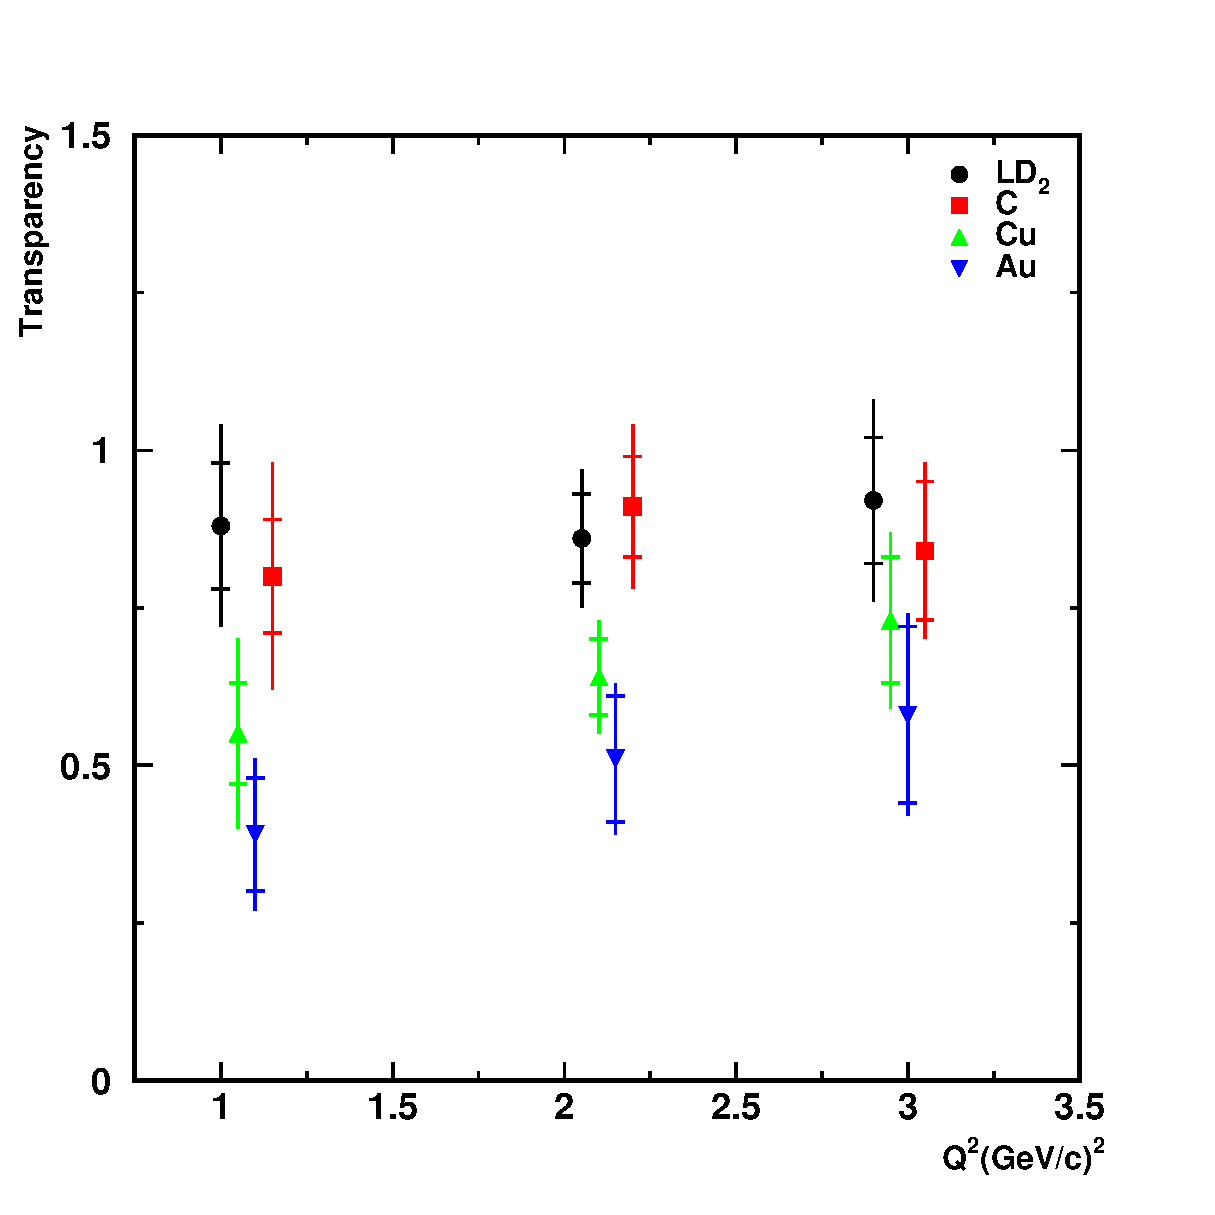
\includegraphics[width=0.8\columnwidth]{transp1}
  \caption[Nuclear transparency with respect to $H_2$ target.]{\label{fig:transp1}Nuclear transparency with respect to $H_2$ target.\\\\ Copper, carbon and $LD_2$ are shifted by -0.05, 0.05 and -0.10 $(\mathrm{GeV/c})^2$ in $Q^2$, respectively, for convenience.}
\end{figure}
%\setlength{\figwidth}{0.8\linewidth}
%\Figure{transp1}{\figwidth}{Nuclear transparency for different targets. Copper, carbon and $LD_2$ are shifted by -0.05, 0.05 and -0.10 $(\mathrm{GeV/c})^2$ in $Q^2$, respectively, for convenience.}

\Table{t_1}{Cross section for hydrogen for different $Q^2$ for kaons.}

%\begin{table}
%  \caption[T and $\sigma_{eff}$ for different targets with respect to $H_2$.]{\label{tab:t_2}T and $\sigma_{eff}$ for different targets with respect to $H_2$.\\\\ Different kinematic settings for kaons with respect to the free space cross section are shown here.}
%\begin{center}
\begin{tabular}{||c|c|c|c|c|c|c||}\hline
 Target & $Q^2$ & Cross section & Transparency & Statistical & Systematic & Total \\
 & $(GeV/c)^2$ & (mb) & & error($\%$)& error($\%$)&error($\%$) \\\hline
$LD_2$ & 1.1 & 8.38 & 0.88 & 10.30 & 12.34 & 16.07\\
Carbon & 1.1 & 7.57 & 0.80 & 09.31 & 16.11 & 18.61\\
Copper & 1.1 & 5.17 & 0.55 & 07.85 & 12.69 & 14.92\\
Gold   & 1.1 & 3.64 & 0.39 & 09.03 & 07.13 & 11.51\\\hline
$LD_2$ & 2.2 & 7.53 & 0.86 & 07.51 & 07.48 & 10.61\\
Carbon & 2.2 & 8.01 & 0.91 & 07.58 & 10.03 & 12.57\\
Copper & 2.2 & 5.60 & 0.64 & 06.45 & 06.43 & 09.11\\
Gold   & 2.2 & 4.49 & 0.51 & 09.93 & 06.40 & 11.82\\\hline
$LD_2$ & 3.0 & 8.55 & 0.92 & 10.22 & 12.06 & 15.81\\
Carbon & 3.0 & 7.76 & 0.84 & 11.49 & 08.10 & 14.06\\
Copper & 3.0 & 6.75 & 0.73 & 10.24 & 09.33 & 13.85\\
Gold   & 3.0 & 5.42 & 0.58 & 13.91 & 08.22 & 16.16\\\hline
\end{tabular}
\end{center}
%\end{table}
\Table{t_2}{T and $\sigma_{eff}$ for different targets with respect to $H_2$.}

\Table{t_3}{Cross section for deuterium for different $Q^2$ for kaons.} %content of appendix
%\newpage %end of appendix title page

\chapter{Miscellaneous} %for a single appendix
\newpage %end of appendix title page
\Section{$\alpha$ Plot}
%\label{$\alpha$ plot}
We have shown $\alpha$ for three kinematic settings in \Tableref{alpha1} plotted in BLUE in \figureref{alpha} with respect to hydrogen target. The available $\alpha$ values from proton and pion analysis have been shown in RED and GREEN, respectively, for comparison. We considered only the statistical uncertainties which are shown by closed vertical lines. The experimental $\alpha$ values from the processes other than electro-production are shown by the horizontal band in \figureref{alpha}. The width of the band represents statistical uncertainty.

\begin{figure}[!tbp]
  \centering
  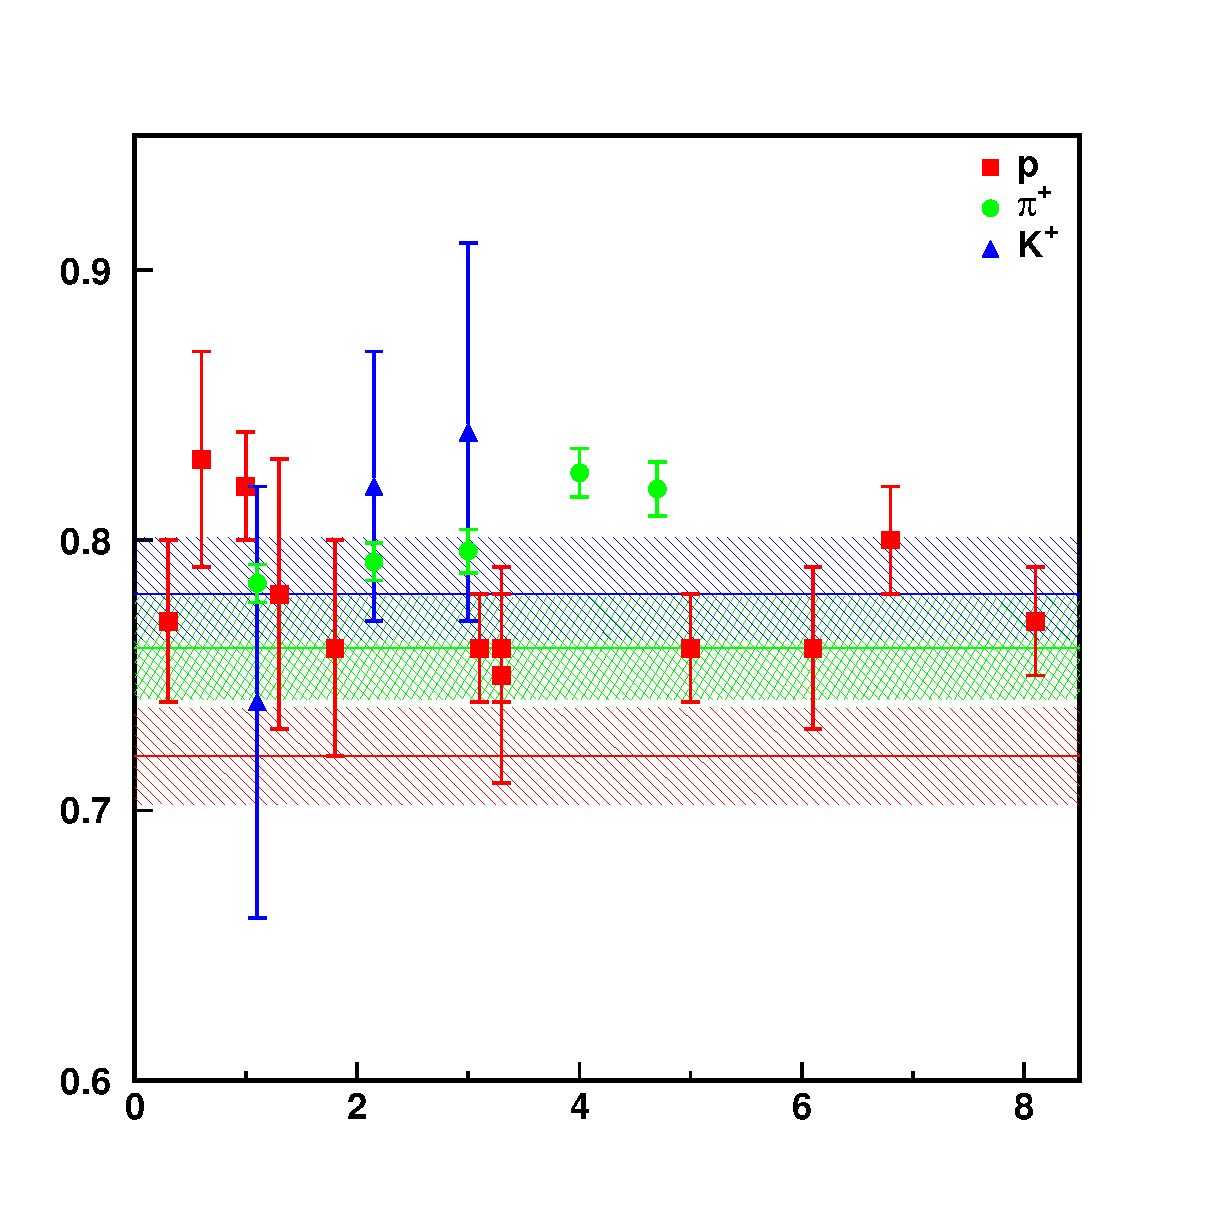
\includegraphics[trim = 8mm 8mm 8mm 8mm, clip,width=0.8\columnwidth]{alpha}
  \caption[$\alpha$ for different kinematics electro-production and hadro-production.]{\label{fig:alpha}$\alpha$ for different kinematics electro-production and hadro-production.\\\\ Electro-production data points in RED are for protons, GREEN data points are for $\pi^+$ and BLUE data points are from this analysis for $K^+$. Similarly, horizontal lines corresponds to $\alpha$ values from hadron-scattering with error band for different hadrons.}
\end{figure}
%\Figure{alpha}{\figwidth}{$\alpha$ for different kinematics electro-production and hadro-production. Electro-production data points in \textcolor{red}{RED} are for protons, \textcolor{green}{GREEN} data points are for $\pi^+$ and \textcolor{blue}{BLUE} data points are from this analysis for $K^+$. Similarly, horizontal lines corresponds to $\alpha$ values from hadron-scattering with error band for different hadrons.}
\begin{table}
  \caption{$\alpha$ values for different $Q^2$ for kaons with respect to hydrogen.}
  \label{tab:alpha1}
\include{alpha1}
\end{table}
%\Table{alpha1}{$\alpha$ values for different $Q^2$ for kaons with respect to hydrogen.}
\newpage
\Section{Comparison of Yields for Data with SIMC}
We already discussed in section \ref{Comparison of Data with SIMC Yields} about the dependency of the cross section upon four variables: $Q^2$, $W$, $t$ and $\phi_{pq}$, where $Q^2$ is four-momentum transferred square, $W$ is the center of mass energy, $t$ is momentum transfer, and $\phi_{pq}$ is  the angle between the scattering and reaction planes. In this appendix, we are showing comparison of SIMC and data yields for missing mass, $W$, $t$ and $\phi_{pq}$ in the \figureref{missmass2}, \figureref{com_plot_w_2}, \figureref{com_plot_t_2} and \figureref{com_plot_phi_2}, respectively. We have already shown the comparison for $Q^2$ in section \ref{Comparison of Data with SIMC Yields}.

\begin{figure}[!tbp]
  \centering
  \includegraphics[width=0.8\columnwidth]{missmass2}
  \caption[Missing mass are shown here after applying cuts.]{\label{fig:missmass2}Missing mass are shown here after applying cuts.\\\\ One-dimensional plot of missing mass are shown here after applying all the cuts. Clockwise top left corner: $M_\Lambda^{SIMC}$ and $M_\Sigma^{SIMC}$ in RED, $M_\Sigma^{data}$ and $M_\Lambda^{data}$ in BLUE for $Q^2$=2.2 $(\mathrm{GeV/c})^2$.}
\end{figure}
%\Figure{missmass2}{\figwidth}{One-dimensional plot of missing mass are shown here after applying cuts. Clockwise top left corner: $M_\Lambda^{SIMC}$ and $M_\Sigma^{SIMC}$ in \textcolor{red}{RED}, $M_\Sigma^{data}$ and $M_\Lambda^{data}$ in \textcolor{blue}{BLUE}.}

\begin{figure}[!tbp]
  \centering
  \includegraphics[width=0.8\columnwidth]{com_plot_w_2}
  \caption[Comparison of $W$ from data and SIMC.]{\label{fig:com_plot_w_2}Comparison of $W$ from data and SIMC.\\\\ Clockwise from top left corner: $W_\Lambda$ and $W_\Sigma$ SIMC in RED, $W_\Sigma$ and $W_\Lambda$ data in BLUE for $Q^2$=2.2 $(\mathrm{GeV/c})^2$.}
\end{figure}
%\setlength{\figwidth}{0.8\linewidth}
%\Figure{com_plot_w_2}{\figwidth}{$W$. Clockwise from top left corner: $W_\Lambda$ and $W_\Sigma$ SIMC in \textcolor{red}{RED}, $W_\Sigma$ and $W_\Lambda$ data in \textcolor{blue}{BLUE} for $Q^2$=2.2 $(\mathrm{GeV/c})^2$.}

\begin{figure}[!tbp]
  \centering
  \includegraphics[width=0.8\columnwidth]{com_plot_t_2}
  \caption[Comparison of $t$ from data and SIMC.]{\label{fig:com_plot_t_2}Comparison of $t$ from data and SIMC.\\\\ Clockwise from top left corner: $t_\Lambda$ and $t_\Sigma$ SIMC in RED, $t_\Sigma$ data and $t_\Lambda$ data in BLUE for $Q^2$=2.2 $(\mathrm{GeV/c})^2$.}
\end{figure}
%\setlength{\figwidth}{0.8\linewidth}
%\Figure{com_plot_t_2}{\figwidth}{$t$. Clockwise from top left corner: $t_\Lambda$ and $t_\Sigma$ SIMC in \textcolor{red}{RED}, $t_\Sigma$ data and $t_\Lambda$ data in \textcolor{blue}{BLUE} for $Q^2$=2.2 $(\mathrm{GeV/c})^2$.}

\begin{figure}[!tbp]
  \centering
  \includegraphics[width=0.8\columnwidth]{com_plot_phi_2}
  \caption[Comparison of $\phi^{pq}$ from data and SIMC.]{\label{fig:com_plot_phi_2}Comparison of $\phi^{pq}$ from data and SIMC.\\\\ Clockwise from top left corner: $\phi^{pq}_\Lambda$ and $\phi^{pq}_\Sigma$ SIMC shown in RED, $\phi^{pq}_\Sigma$ data and $\phi^{pq}_\Lambda$ data in BLUE for $Q^2$=2.2 $(\mathrm{GeV/c})^2$.}
\end{figure}
%\setlength{\figwidth}{0.8\linewidth}
%\Figure{com_plot_phi_2}{\figwidth}{$\phi^{pq}$. Clockwise from top left corner: $\phi^{pq}_\Lambda$ and $\phi^{pq}_\Sigma$ SIMC shown in \textcolor{red}{RED}, $\phi^{pq}_\Sigma$ data and $\phi^{pq}_\Lambda$ data in \textcolor{blue}{BLUE} for $Q^2$=2.2 $(\mathrm{GeV/c})^2$.}

\Section{Iteration}
We have done the iteration on the data to verify our transparency results. As the statistics was very low, we did not expect a large variation in the results. We fitted data for the variables $Q^2$, $W$ and t for $\Lambda$ and $\Sigma$ production as shown in \figureref{fitfunction_kin2_1}, \figureref{fitfunction_kin2_2} and \figureref{fitfunction_kin2_3}, respectively. These fit functions were used to generate the SIMC ntuples. New ntuples were used again for extraction of transparency to check the stability of the yields. This process was repeated doing a second iteration. After the iteration, we did not get any reasonable change in the yields and hence results presented in this thesis are without considering any iteration.

\begin{figure}[!tbp]
  \centering
  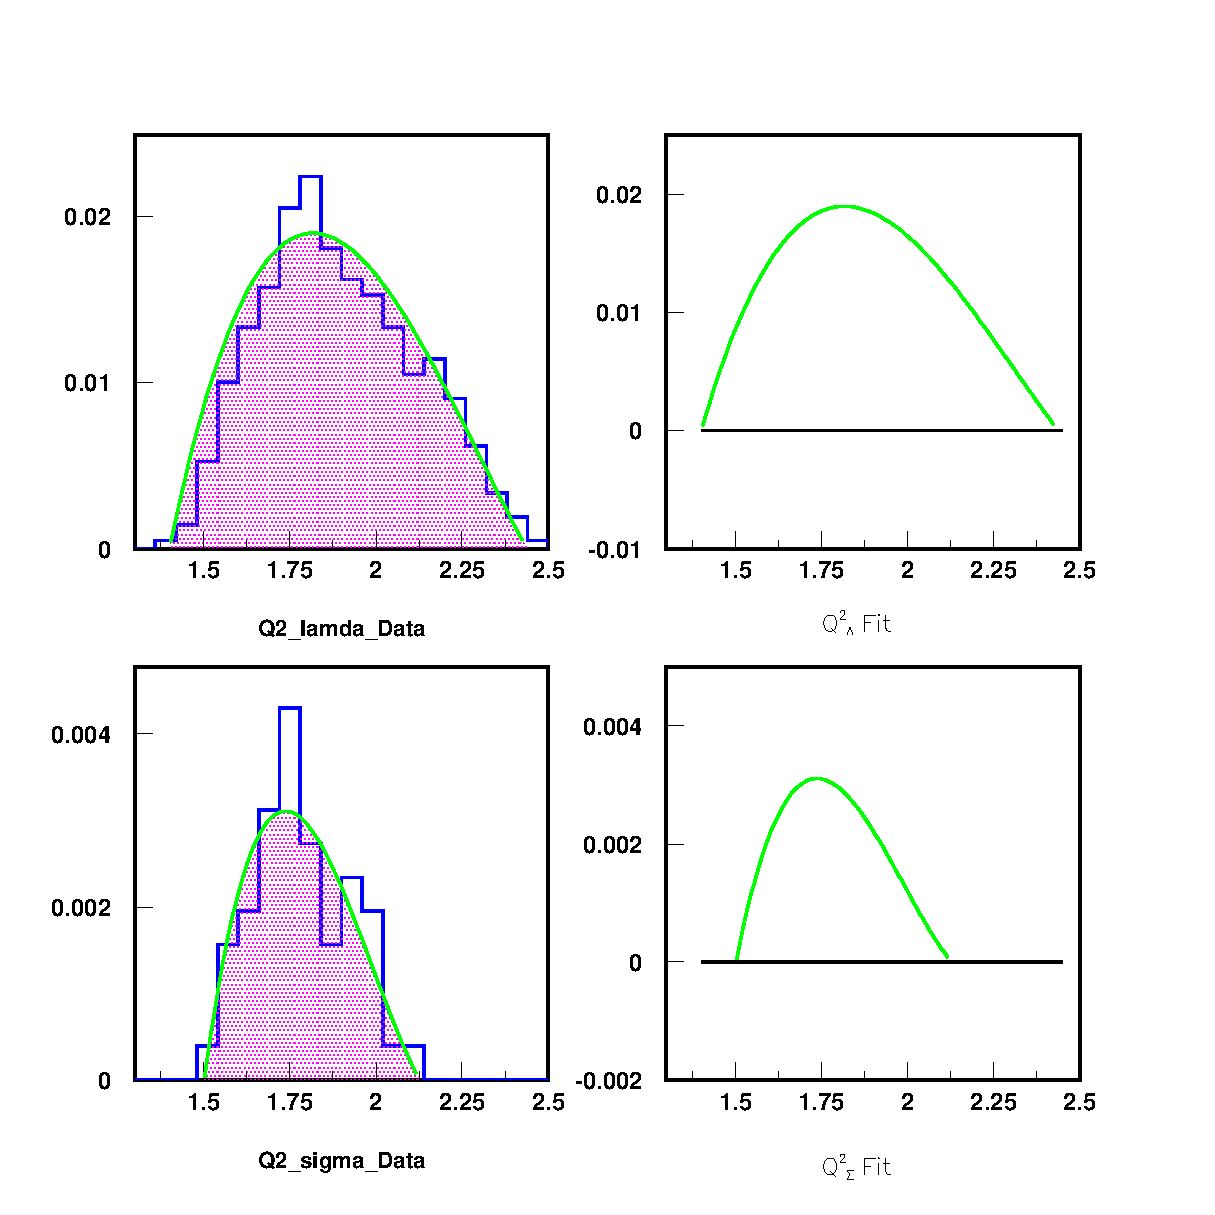
\includegraphics[width=0.8\columnwidth]{fitfunction_kin2_1}
  \caption[Fitting $Q^2$ for iteration.]{\label{fig:fitfunction_kin2_1}Fitting the $Q^2$ data for kinematic settings of $Q^2$=2.2 $(\mathrm{GeV/c})^2$ for iteration.}
\end{figure}
%\setlength{\figwidth}{0.8\linewidth}
%\Figure{fitfunction_kin2_1}{\figwidth}{Fitting the $Q^2$ data for kinematic settings of $Q^2$=2.2 $(\mathrm{GeV/c})^2$ for iteration.}

\begin{figure}[!tbp]
  \centering
  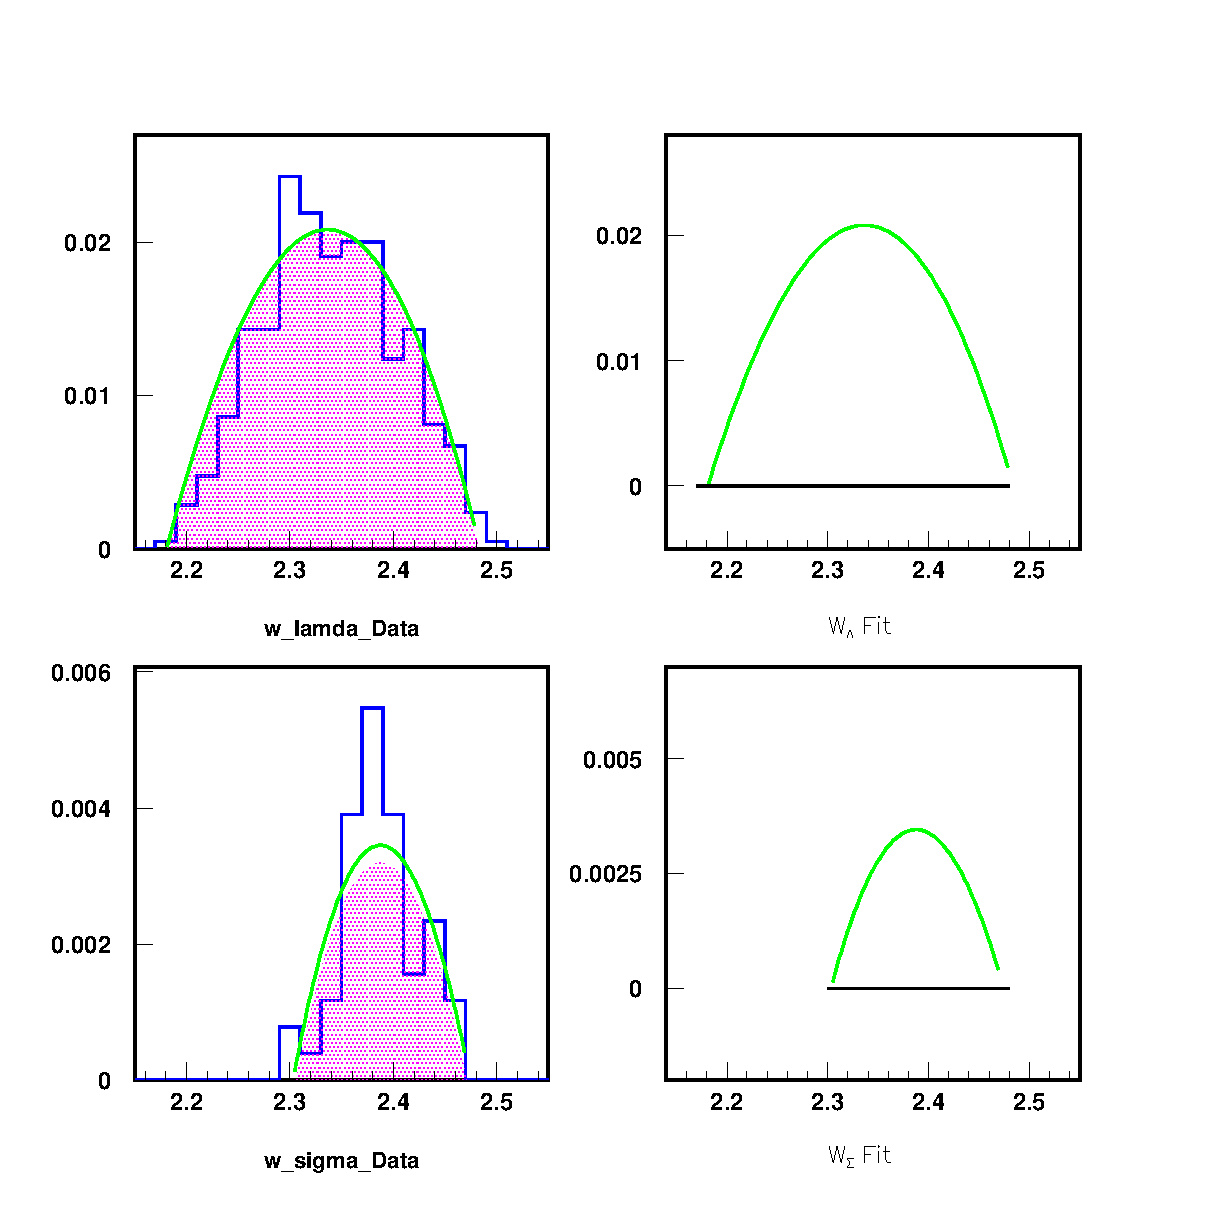
\includegraphics[width=0.8\columnwidth]{fitfunction_kin2_2}
  \caption[Fitting $W$ for iteration.]{\label{fig:fitfunction_kin2_2}Fitting the $W$ data for kinematic settings of $Q^2$=2.2 $(\mathrm{GeV/c})^2$ for iteration.}
\end{figure}
%\setlength{\figwidth}{0.8\linewidth}
%\Figure{fitfunction_kin2_2}{\figwidth}{Fitting the W data for kinematic settings of $Q^2$=2.2 $(\mathrm{GeV/c})^2$ for iteration.}

\begin{figure}[!tbp]
  \centering
  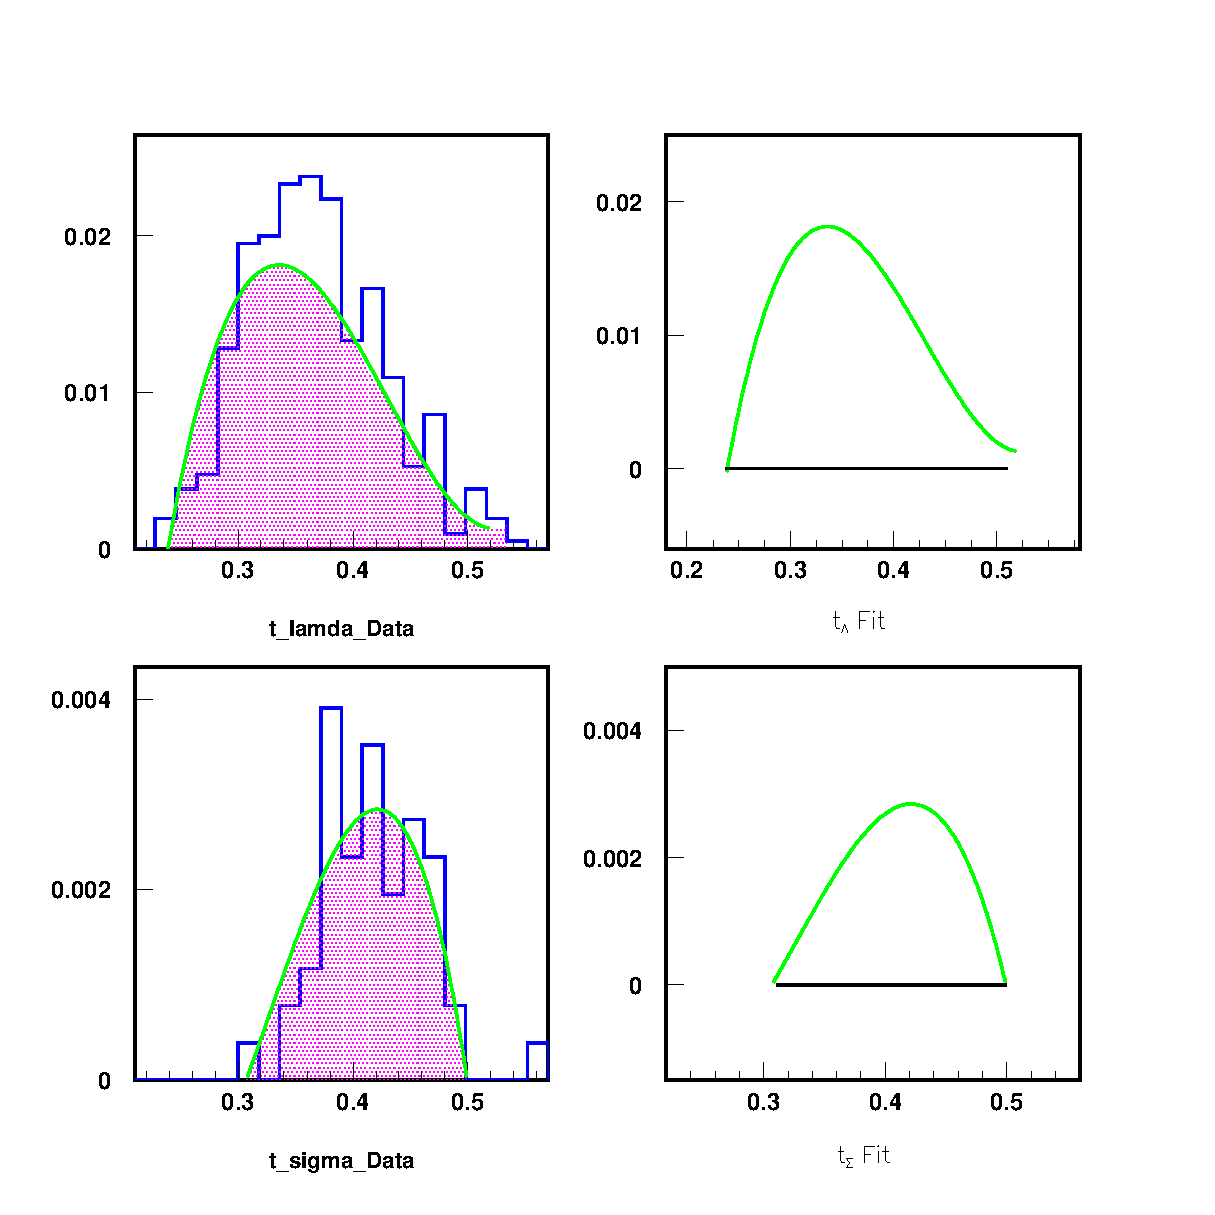
\includegraphics[width=0.8\columnwidth]{fitfunction_kin2_3}
  \caption[Fitting $t$ for iteration.]{\label{fig:fitfunction_kin2_3}Fitting the $t$ data for kinematic settings of $Q^2$=2.2 $(\mathrm{GeV/c})^2$ for iteration.}
\end{figure}
%\setlength{\figwidth}{0.8\linewidth}
%\Figure{fitfunction_kin2_3}{\figwidth}{Fitting the $t$ data for kinematic settings of $Q^2$=2.2 $(\mathrm{GeV/c})^2$ for iteration.} %content of appendix
%\chapter{An Appendix Title} %alternative for each of multiple appendices

%\newpage %end of appendix title page


\end{document}
